%%%%%%%%%%%%%%%%%%%%%%%%%%%%%%%%%%%%%%%%%
% Masters/Doctoral Thesis 
% LaTeX Template
% Version 2.3 (25/3/16)
%
% This template has been downloaded from:
% http://www.LaTeXTemplates.com
%
% Version 2.x major modifications by:
% Vel (vel@latextemplates.com)
%
% This template is based on a template by:
% Steve Gunn (http://users.ecs.soton.ac.uk/srg/softwaretools/document/templates/)
% Sunil Patel (http://www.sunilpatel.co.uk/thesis-template/)
%
% Template license:
% CC BY-NC-SA 3.0 (http://creativecommons.org/licenses/by-nc-sa/3.0/)
%
%%%%%%%%%%%%%%%%%%%%%%%%%%%%%%%%%%%%%%%%%

%----------------------------------------------------------------------------------------
%    PACKAGES AND OTHER DOCUMENT CONFIGURATIONS
%----------------------------------------------------------------------------------------

\documentclass[
11pt, % The default document font size, options: 10pt, 11pt, 12pt
%oneside, % Two side (alternating margins) for binding by default, uncomment to switch to one side
%chapterinoneline,% Have the chapter title next to the number in one single line
english, % ngerman for German
singlespacing, % Single line spacing, alternatives: onehalfspacing or doublespacing
%draft, % Uncomment to enable draft mode (no pictures, no links, overfull hboxes indicated)
%nolistspacing, % If the document is onehalfspacing or doublespacing, uncomment this to set spacing in lists to single
%liststotoc, % Uncomment to add the list of figures/tables/etc to the table of contents
%toctotoc, % Uncomment to add the main table of contents to the table of contents
%parskip, % Uncomment to add space between paragraphs
%nohyperref, % Uncomment to not load the hyperref package
headsepline, % Uncomment to get a line under the header
]{main} % The class file specifying the document structure

\usepackage[utf8]{inputenc} % Required for inputting international characters
\usepackage[T1]{fontenc} % Output font encoding for international characters
\usepackage{palatino} % Use the Palatino font by default
\usepackage[backend=bibtex,style=authoryear,natbib=true]{biblatex} % Use the bibtex backend with the authoryear citation style (which resembles APA)
\usepackage[autostyle=true]{csquotes} % Required to generate language-dependent quotes in the bibliography

%----------------------------------------------------------------------------------------
%    RapMap Packages
%----------------------------------------------------------------------------------------
\usepackage[justification=centering]{caption}
\usepackage{xspace}
\usepackage{bm}
\usepackage{microtype}
% \usepackage{xifthen}
\usepackage{amsmath}
\usepackage{amssymb}
\usepackage{amstext}
\usepackage{amsthm}
% \usepackage{graphicx}
% \usepackage{booktabs}
% \usepackage[normalem]{ulem}
% \usepackage{setspace}
\usepackage{tabulary}
\usepackage{tablefootnote}
% \usepackage{float}
% \usepackage{natbib}
% \usepackage{newfloat}
\usepackage{cleveref}
\usepackage{footmisc}

%----------------------------------------------------------------------------------------
%    MARGIN SETTINGS
%----------------------------------------------------------------------------------------
\addbibresource{main.bib} % The filename of the bibliography

\geometry{
    paper=a4paper, % Change to letterpaper for US letter
    inner=2.5cm, % Inner margin
    outer=3.8cm, % Outer margin
    bindingoffset=2cm, % Binding offset
    top=1.5cm, % Top margin
    bottom=1.5cm, % Bottom margin
    %showframe,% show how the type block is set on the page
}

%----------------------------------------------------------------------------------------
%    THESIS INFORMATION
%----------------------------------------------------------------------------------------

\thesistitle{Efficient quantification of bulk and droplet-based single-cell RNA-sequencing data}
% Your thesis title, this is used in the title and abstract, print it elsewhere with \ttitle
\supervisor{Prof. Rob \textsc{Patro} } % Your supervisor's name, this is used in the title page, print it elsewhere with \supname
\examinerO{Prof. Michael \textsc{Bender}} % Your examiner's name, this is not currently used anywhere in the template, print it elsewhere with \examname
\examinerTh{Prof. Steve \textsc{Skiena}} % Your examiner's name, this is not currently used anywhere in the template, print it elsewhere with \examname
\degree{Doctor of Philosophy} % Your degree name, this is used in the title page and abstract, print it elsewhere with \degreename
\author{Avi \textsc{Srivastava}} % Your name, this is used in the title page and abstract, print it elsewhere with \authorname
\addresses{} % Your address, this is not currently used anywhere in the template, print it elsewhere with \addressname

\subject{Computational Biology} % Your subject area, this is not currently used anywhere in the template, print it elsewhere with \subjectname
\keywords{RNA-seq, dscRNA-seq, quantification, quasi-mapping, UMI-deduplication} % Keywords for your thesis, this is not currently used anywhere in the template, print it elsewhere with \keywordnames
\university{\href{http://www.stonybrook.edu/}{Stony Brook University}} % Your university's name and URL, this is used in the title page and abstract, print it elsewhere with \univname
\department{\href{https://www.cs.stonybrook.edu/}{Department of Computer Science}} % Your department's name and URL, this is used in the title page and abstract, print it elsewhere with \deptname
\group{\href{http://combine-lab.github.io/}{Combine-Lab}} % Your research group's name and URL, this is used in the title page, print it elsewhere with \groupname
\faculty{\href{http://www.robpatro.com/redesign/}{Rob Patro}} % Your faculty's name and URL, this is used in the title page and abstract, print it elsewhere with \facname

\hypersetup{pdftitle=\ttitle} % Set the PDF's title to your title
\hypersetup{pdfauthor=\authorname} % Set the PDF's author to your name
\hypersetup{pdfkeywords=\keywordnames} % Set the PDF's keywords to your keywords

\begin{document}

\frontmatter % Use roman page numbering style (i, ii, iii, iv...) for the pre-content pages

\pagestyle{plain} % Default to the plain heading style until the thesis style is called for the body content

%----------------------------------------------------------------------------------------
%    TITLE PAGE
%----------------------------------------------------------------------------------------

\begin{titlepage}
\begin{center}

{\scshape\LARGE \univname\par}\vspace{1.5cm} % University name
\textsc{\Large Preliminary Examination --- Defense Proposal}\\[0.5cm] % Thesis type

\HRule \\[0.4cm] % Horizontal line
{\huge \bfseries \ttitle\par}\vspace{0.4cm} % Thesis title
\HRule \\[1.5cm] % Horizontal line
 
\begin{minipage}[t]{0.4\textwidth}
\begin{flushleft} \large
\emph{Author:}\\
\href{http://k3yavi.github.io/}{\authorname} % Author name - remove the \href bracket to remove the link
\end{flushleft}
\end{minipage}
\begin{minipage}[t]{0.4\textwidth}
\begin{flushright} \large
\emph{Committee:} \\
\href{http://www.robpatro.com/redesign/}{\supname  (Advisor)}\\ % Supervisor name - remove the \href bracket to remove the link 
\href{http://www3.cs.stonybrook.edu/~bender/}{\examinerOname}\\
\href{https://www3.cs.stonybrook.edu/~skiena/}{\examinerThname}
\end{flushright}
\end{minipage}\\[3cm]
 
\large \textit{A Preliminary report submitted in partial fulfillment of the requirements\\ for the degree of \degreename}\\[0.3cm] % University requirement text
\textit{in the}\\[0.4cm]
\groupname\\\deptname\\[2cm] % Research group name and department name
 
{\large \today}\\[4cm] % Date
%\includegraphics{Logo} % University/department logo - uncomment to place it
 
\vfill
\end{center}
\end{titlepage}

%----------------------------------------------------------------------------------------
%    DECLARATION PAGE
%----------------------------------------------------------------------------------------

% \begin{declaration}
% \addchaptertocentry{\authorshipname}
%
% \noindent I, \authorname, declare that this report titled, \enquote{\ttitle} and the work presented in it are my own. I confirm that:
%
% \begin{itemize}
% \item This work was done wholly or mainly while in candidature for a research degree at this University.
% \item Where any part of this thesis has previously been submitted for a degree or any other qualification at this University or any other institution, this has been clearly stated.
% \item Where I have consulted the published work of others, this is always clearly attributed.
% \item Where I have quoted from the work of others, the source is always given. With the exception of such quotations, this thesis is entirely my own work.
% \item I have acknowledged all main sources of help.
% \item Where the thesis is based on work done by myself jointly with others, I have made clear exactly what was done by others and what I have contributed myself.\\
% \end{itemize}
%
% \noindent Signed:\\
% \rule[0.5em]{25em}{0.5pt} % This prints a line for the signature
%
% \noindent Date:\\
% \rule[0.5em]{25em}{0.5pt} % This prints a line to write the date
% \end{declaration}
%
% \cleardoublepage

%----------------------------------------------------------------------------------------
%    QUOTATION PAGE
%----------------------------------------------------------------------------------------

\vspace*{0.2\textheight}

\noindent\enquote{\itshape Nature uses only the longest threads to weave her patterns so that each small piece of her fabric reveals the organization of the entire tapestry.}\bigbreak

\hfill Richard Feynman

%----------------------------------------------------------------------------------------
%    ABSTRACT PAGE
%----------------------------------------------------------------------------------------

\begin{abstract}
\addchaptertocentry{\abstractname} % Add the abstract to the table of contents

RNA Sequencing (RNA-seq) technologies are evolving rapidly, and with them, the requirement 
for fast and accurate tools to analyze the generated data. The first step of many RNA-seq
analyses require us to solve the problem of \ra. When reads are aligned to a collection of 
reference sequences that share a substantial amount of sub-sequence (near or exact repeats), 
a single read can have many potential alignments, and considering all such alignment can be 
crucial for downstream analysis like quantification. This dissertation discusses the evolution of 
the tools developed to handle the problem of \ra for next-generation sequencing, their impact 
on RNA-seq analysis, introduce a novel concept, \qm, and an efficient algorithm implementing 
this approach called \rapmap which maps RNA-seq \reads (sequences) to the reference sequence(s) 
(transcriptome). By attempting only to report the potential loci of origin of a sequencing read, 
and not the base-to-base alignment by which it derives from the reference, \rapmap is capable of 
\textit{mapping} sequencing reads to a target transcriptome substantially faster than existing 
alignment tools. The algorithm we employ to implement \qm uses several efficient data structures 
and takes advantage of the special structure of shared sequence prevalent in transcriptomes to 
rapidly provide highly-accurate mapping information.

While bulk RNA-sequencing is an established method to perform genome-wide quantification of gene 
expressions, however, quantification tools for bulk RNA-seq cannot be directly used for 
droplet-based single-cell RNA-sequencing (dscRNA-seq) data. We introduce alevin, a fast 
end-to-end pipeline to process droplet-based single-cell RNA sequencing data, performing 
cell barcode detection, read mapping, unique molecular identifier (UMI) deduplication, 
gene count estimation, and cell barcode whitelisting. Alevin’s approach to UMI deduplication 
considers transcript-level constraints on the molecules from which UMIs may have arisen and 
accounts for both gene-unique reads and reads that multimap between genes. This addresses 
the inherent bias in existing tools which discard gene-ambiguous reads and improves the 
accuracy of gene abundance estimates. Alevin is considerably faster, typically 8 times  
than existing gene-quantification approaches, while also using less memory.

Finally, we propose to generalize both methods to make them more robust and extend their capabilities. 
While \qm is a useful novel concept, it trades-off some accuracy for speed. This does not have a huge
impact on typical RNA-seq experiments. However, in \textit{relatively} complex datasets, the loss in accuracy 
can be significant. In ongoing work, we have updated \rapmap to employ alignments to improve 
quantifications in an efficient, dynamic (dataset dependent) way. This optimizes the
speed/accuracy tradeoff, making the estimates almost as accurate as end-to-end alignment-based
methods, while still using resources similar to \rapmap. Moreover, we propose a principled approach and 
study the effect of further extending \alevin's UMI deduplication algorithm to include unspliced RNA.

\end{abstract}

%----------------------------------------------------------------------------------------
%    ACKNOWLEDGEMENTS
%----------------------------------------------------------------------------------------

\begin{acknowledgements}
\addchaptertocentry{\acknowledgementname} % Add the acknowledgements to the table of contents

My experience as a Ph.D. student at Stony Brook has been life changing as it has helped me 
grow both personally and professionally. A big fraction of that is due to my advisor, 
Rob Patro, whom I'd like to thank for his patience, guidance, and encouragement for letting 
me explore the field of computational biology.
Working with him has been very exciting as he taught me how to do science. His vision 
and tenaciousness to work and improve the RNA-seq quantification has helped me learn, 
how looking at a problem from many different angles generate exciting new ideas. I also 
feel, his love for statically-typed programmed programming languages has helped me realize 
the importance of designing efficient tools which I hope to keep for the rest of my career.

I'd like to thank other members of my committee, Steve Skiena and Michael Bender whose 
important contributions through various lectures, talks, and feedback on this dissertation has 
been pivotal for my cademic development while at Stony Brook university. I'm honored to 
have them as my committee members.

I'm very grateful to my colleagues and it was an exciting experience to learn and grow
alongside them over the years. In particular, Laraib Malik, Hirak sarkar, Mohsen Zakeri, and 
Fatemeh Almodaresi made Combine-Lab an interesting place to work as they helped me by 
providing insightful discussions. I can't imagine working through all the paper deadlines,
had been a more enjoyable and pleasant experience without them. I'd also like to thank Mike Love, 
Charlotte Soneson, Geet Duggal, Richard Smith-Unna, Owen Dando, Darya Filipova, Patrick Marks 
and Paul Ryvkin for their insightful discussions regarding various aspects of the work.

I couldn't thank enough to my family for their support throughout my journey of learning. 
Especially my father, Y K Srivastava, who guided me from my childhood to learn and motivate me 
to think out-of-box. I'd like to thank my mother Ritima Srivastava, brother Prakhar Srivastava,
late grandparents, Govind Prasad Srivastava, Savitri Srivastava, and all my cousins brother and
sister for providing the comfortable and loving environment they provided for me growing up. 

At last, I would also like to thank Stony Brook Research Computing and 
Cyberinfrastructure, and the Institute for Advanced Computational Science at Stony Brook 
University for access to the high-performance SeaWulf computing system, which was made 
possible by a National Science Foundation grant (\#1531492).
\end{acknowledgements}

%----------------------------------------------------------------------------------------
%    LIST OF CONTENTS/FIGURES/TABLES PAGES
%----------------------------------------------------------------------------------------

\tableofcontents % Prints the main table of contents

\listoffigures % Prints the list of figures

\listoftables % Prints the list of tables

% ----------------------------------------------------------------------------------------
%     ABBREVIATIONS
% ----------------------------------------------------------------------------------------

\begin{abbreviations}{ll} % Include a list of abbreviations (a table of two columns)

\textbf{ARD} & \textbf{A}bsolute  \textbf{R}elative \textbf{D}ifference\\
\textbf{BLAST} & \textbf{B}asic \textbf{L}ocal \textbf{A}lignment \textbf{S}earch \textbf{T}ool\\
\textbf{BWT} & \textbf{B}urrows-\textbf{W}heeler \textbf{T}ransform\\
\textbf{DFS} & \textbf{D}epth-\textbf{F}irst \textbf{S}earch\\
\textbf{DP} & \textbf{D}ynamic-\textbf{P}rogram\\
\textbf{Indel} & \textbf{In}setion (and) \textbf{D}eletion\\
\textbf{MARD} & \textbf{M}ean \textbf{A}bsolute  \textbf{R}elative \textbf{D}ifference\\
\textbf{NGS} & \textbf{N}ext \textbf{G}eneration \textbf{S}equencing\\
\textbf{SA} & \textbf{S}uffix \textbf{A}rray\\
\textbf{SGS} & \textbf{S}econd \textbf{G}eneration \textbf{S}equencing\\
\textbf{SIMD} & \textbf{S}ingle \textbf{I}nstruction \textbf{M}ultiple \textbf{D}ata\\
\textbf{SMEM} & \textbf{S}uper \textbf{M}aximal \textbf{E}xact \textbf{M}atch\\
\textbf{T-DBG} & \textbf{T}ranscriptome - \textbf{d}e \textbf{B}ruijn \textbf{G}raph\\
\textbf{TPEF} & \textbf{T}rue \textbf{P}ositive \textbf{E}rror \textbf{F}raction\\
\textbf{TPME} & \textbf{T}rue \textbf{P}ositive  \textbf{M}edian \textbf{E}rror\\
\textbf{VBEM} & \textbf{V}ariational \textbf{B}ayesian - \textbf{E}xpectation \textbf{M}aximization\\
\textbf{wMARD} & \textbf{w}eighted \textbf{M}ean \textbf{A}bsolute  \textbf{R}elative \textbf{D}ifference\\
\textbf{dscRNA-seq} & \textbf{d}roplet based \textbf{s}ingle \textbf{c}ell  \textbf{RNA}-seq\\
\textbf{CB} & \textbf{C}ellular \textbf{B}arcode\\
\textbf{UMI} & \textbf{U}nique \textbf{M}olecule \textbf{I}dentifier\\
\textbf{PUG} & \textbf{P}arsimonious \textbf{U}MI \textbf{G}raph\\

\end{abbreviations}

%----------------------------------------------------------------------------------------
%    PHYSICAL CONSTANTS/OTHER DEFINITIONS
%----------------------------------------------------------------------------------------

% \begin{constants}{lr@{${}={}$}l} % The list of physical constants is a three column table
%
% % The \SI{}{} command is provided by the siunitx package, see its documentation for instructions on how to use it
%
%     Speed of Light & $c_{0}$ & \SI{2.99792458e8}{\meter\per\second} (exact)\\
% %Constant Name & $Symbol$ & $Constant Value$ with units\\
%
% \end{constants}

%----------------------------------------------------------------------------------------
%    SYMBOLS
%----------------------------------------------------------------------------------------

% \begin{symbols}{lll} % Include a list of Symbols (a three column table)
%
% $a$ & distance & \si{\meter} \\
% $P$ & power & \si{\watt} (\si{\joule\per\second}) \\
% %Symbol & Name & Unit \\
%
% \addlinespace % Gap to separate the Roman symbols from the Greek
%
% $\omega$ & angular frequency & \si{\radian} \\
%
% \end{symbols}

%----------------------------------------------------------------------------------------
%    DEDICATION
%----------------------------------------------------------------------------------------

% \dedicatory{For/Dedicated to/To my\ldots}

%----------------------------------------------------------------------------------------
%    THESIS CONTENT - CHAPTERS
%----------------------------------------------------------------------------------------

\mainmatter % Begin numeric (1,2,3...) page numbering

\pagestyle{thesis} % Return the page headers back to the "thesis" style

% Include the chapters of the thesis as separate files from the Chapters folder
% Uncomment the lines as you write the chapters

% Chapter 1

\chapter{Introduction} % Main chapter title

\label{intro} % For referencing the chapter elsewhere, use \ref{Chapter1} 

%----------------------------------------------------------------------------------------


DNA sequencing is generally performed in three phases~\citep{schadt2010window}: fragmentation, physical-sequencing, and assembly. The first phase of fragmentation breaks the reference DNA into several small pieces and amplifies it into multiple copies, based on the requirements of the analysis. In the physical sequencing phase, individual units (called \textit{bases}) of the fragments are identified in the sequential order to create a read, the number of the contiguous sequence of bases in a read defines its length measured in base-pairs (bp). In the last phase of assembly, the collection of \reads (called \textit{library}) is analyzed by bioinformatics software to find overlapping regions in a \textit{library} of \reads and create "most of" the contiguous sequences of the genome. The phrase "most of" is particularly important because based on the species, sequencing technology, and many external factors sequencing can face many different biological and computational challenges and can give different results like collapsing the repetitive sequence of the genome.


\begin{figure*}[!htb]
\centering
\includegraphics[width=0.6\textwidth]{{Avi.RPE.fig.4}.pdf}
\caption{From top to bottom: Single-End Sequencing, Paired-End Sequencing, information retained after Paired-End sequencing.}
\label{fig:pe-seq}
\end{figure*}


Physical-sequencing of the \reads is generally performed in either of the two modes: namely single-end (SE) or paired-end (PE). To give the fragments a notion of direction as shown in ~\Cref{fig:pe-seq} fragments are sequenced from 5' end to 3' end (This refers to the 5' and 3' carbons on the sugar presents at each end). In SE sequencing, the fragments are sequenced only from one end. But, in PE sequencing, the fragments are first sequenced from one end for some fixed length, then in another from the opposite end to form a pair of \reads (called \textit{mate-pairs}). Knowing the distance between mate-pairs of a fragment in PE sequencing helps improve the specificity of the alignment of the fragment, especially when the matching region of the read in the genome is not unique. In this case, the distance between its mate-pair can help resolve ambiguity.

Sequencing of the Human Genome~\citep{venter2001sequence} spawned many novel sequencing technologies such as 454 Life sciences (Roche), Illumina (also called Solexa Sequencing), Applied Biosystem's SOLiD, Pacific Biosciences and Oxford Nanopore etc. As a result of these sequencing technologies, scientists have found many biological applications for sequencing a genome, such as studying cancer (cancer genomics), gene regulatory network study and differential expression analysis etc. Most of these biological studies require that we solve the problem of read-alignment before further analysis can be done. Moreover, the accuracy of the downstream analyses greatly depends on how well the problem of read-alignment is solved, which from a computational perspective, makes the problem of read-alignment particularly interesting. The classical problem of \ra and its general mathematical notion can be defined as follows:
\bigbreak
\textbf{Given:} A set of sequence (called \reads) $R$, a reference sequence $T$, a distance function $d(u, v)$ which gives the distance between two sequence $u$ and $v$, and $\epsilon$ (maximum edit distance) where $\epsilon \in \mathbb{Z}^{+}$.\\
\begin{equation}
\label{prboblem}
R = \{ r_i:  r_i \in \Sigma^{l_i}, \Sigma \in \{A,C,G,T\}, i \in [1, n] \}
\end{equation}
where $l_i$ is the length of the \textit{read} $i$ and $n$ is the total number of \reads.\\

\begin{equation}
T = \Sigma^k, \Sigma \in \{A,C,G,T\}
\end{equation}
where $k$ is the length of the reference sequence.\\

\begin{equation}
d:\Sigma^{|u|}\times\Sigma^{|v|}\rightarrow\mathbb{Z} 
\end{equation}

% \textbf{Exact Match Problem: \label{prb:exact}} Find $\forall r_i \in R$, a set of positions $ P = \{p : p \in \{[1, k] \cup {\phi}\footnote{\label{note1}Represents no match condition.}\} \}$ in $T$ where the sequence $r_i$ and the substring of $T$ starting at each position(s) $p \in P$, are the same.\\

\textbf{Read Alignment Problem:} Find $\forall r_i \in R$, a set of tuples $S = \{(s, p, c):  p \in \{[1, k] \cup \emptyset\footnote{\label{note1}Represents no match condition.} \} \}$ such that substring $s$ of $T$ starting from a position $p$, can be generated from $r_i$ using the transformation defined by $c$ (commonly encoded as \textit{CIGAR string}) where $d(r_i, s) \leq \epsilon$ and $c$ represents a edit script.

\bigbreak

Sequencing technology has evolved very quickly and already has three major generation of sequencers. Sanger-sequencing (First Generation sequencing)~\citep{sanger1975rapid} was developed by Sanger in 1975 and produces \reads of 1000 bp . Second generation sequencing (SGS)~\citep{reis2009next} (sometimes called Next Generation Sequencing) technologies can produce 35bp-400bp~\citep{schatz2010assembly} \reads with very high throughput and much lower per base cost than Sanger-sequencing. Third generation sequencing~\citep{schadt2010window}(TGS) has its own advantage of read length which is tens of thousand of bp. TGS suffers from a relatively high error rate and produces comparatively fewer reads than NGS, which is important in certain applications requiring high coverage. 

The bioinformatics community has put tremendous efforts into building a wide array of different tools to solve the problem of \ra, based on the generation of the sequencer these tools use many different strategies to quickly find potential alignment for the \reads. Since the field is being explored intensively, it is very hard to discuss all the tools, we have restricted the literature of the report to SGS tools only and discussed them chronologically on the basis of major methodological advancement over previously developed tools in their time.

\section{Smith-Waterman~\citep{smith1981identification}}
The Smith-Waterman~\citep{smith1981identification} algorithm is a classical algorithm for solving the problem of sequence-alignment which allows both mismatches and indels under a given scoring scheme. It guarantees finding optimal alignment under the time bound of $\bm{O(|T|l_i)}$ for each read $r_i$ (notations as described before~\Cref{prboblem}). For a set $R$ of \reads this time bound becomes $\bm{\sum_{r_i \in R}O(|T|l_i)}$ of which mostly spend on filling DP sub-solutions that have no hope of satisfying the edit distance bound of $\epsilon$ and if we use Smith-Waterman directly on the large reference genomes (like Humans) for \ra, it becomes infeasible. Due to the large computational cost of the algorithm and the presence of huge numbers of \reads, motivated scientists to use heuristics (greedy type approach) to solve the problem.

The family of BLAST~\citep{altschul1990basic, altschul1997gapped} algorithms was one such initiative, initially designed for comparing two long sequences but used also for \ra. These algorithms attempt to optimize a specific local similarity measure which uses heuristics to give the similarity $d(u, v)$ between two sequences $u$ and $v$ based on their biological significance. BLAST give approximate alignment results and was more than an order magnitude faster than previous methods with similar accuracy. BLAST follows a hash table based approach for preprocessing the set of \reads and a simple seed-and-extend strategy on the reference sequence to solve the problem of \ra. BLAST maintains a database of a hash table on all the k-means (k length substrings) of the \reads and traverses the reference sequence to find a hit for seed(s) by checking the database of the hash table (called the \textit{index}). BLAST first joins the seeds without gaps and then refines them by Smith-Waterman for gapped alignment. Generally, in a big reference sequence, only a few subsequences have sufficient similarity to the query; BLAST finds these by filtering irrelevant matches using two threshold parameters $S$ and $T$. Each seed's similarity score is checked to determine if it's greater or equal to than the parameter $T$. Then, BLAST tries to extend seed(s) exceeding the threshold using the Smith-Waterman algorithm to get the maximum matching score (under their similarity measure) and reports only those alignments exceeding the similarity threshold $S$.

Even though BLAST approach was faster than existing methods for read-alignment, it has some shortcomings when viewed in the context of NGS. The index needs to be built for every new read, and for alignment BLAST scans through the entire reference sequence many times (once for each query) resulting in large computational requirements. 


\section{MAQ~\citep{maq}} \label{maq}
MAQ was initially developed for NGS technologies which produced tens of millions of 30-40bp \reads. With \reads, this short, most genomes contain repetitive regions or nearly repetitive regions (edit distance $< \epsilon$), at least as long as these \reads. Because of the repetitive regions \reads can align to the reference on multiple positions (called ambiguous alignments) and even a few mutations can make the read align to the wrong location. One of the major shortcomings of the \ra tools was that for a better accuracy a lot of \reads are ignored based on the ambiguity of their alignment. Although conservatively discarding ambiguous \reads simplifies the read-alignment problem, it leaves out the important information from repetitive regions, which is essential for many biological applications. Instead of just ignoring ambiguous \reads, MAQ~\citep{maq} was one of the first tools to use this information. MAQ uses an approach similar to phred~\citep{ewing1998base} base-calling, i.e. not to discard the ambiguous \reads as soon as they are discovered. Instead, for each ambiguously aligned read, MAQ calculates the likelihood of the read being wrongly positioned and assign a quality score to each alignment. Using the posterior error probability of each alignment, more information is retained than just discarding them. In a nutshell, MAQ uses a seed-and-extend type approach for aligning \reads. It builds a hash on \reads, parses the reference for a hits, but with modification in the alignment strategy of assigning a mapping quality score for each alignment (which is a measure of the confidence that a read actually comes from the position it is aligned to). Also, MAQ doesn't scan reference sequence for every read, instead, it builds the index on a set of read and scans the reference a fixed (small) number of times.

To select a seed, the first 28bp of each read are hashed using six templates (12 for paired-end reads), sorted and stored in the form of a hash-table (called the \textit{index}). Then the subsequences of the reference sequence are scanned for a hit in the hash-table of all six templates. For each hit, MAQ assigns a mapping quality score, which is the sum of the qualities of the mismatching bases over the length of the whole read, extending from the initial 28bp seed without a gap and with at most 2 mismatches. Later, orphaned alignments (mate-pairs where only one mate gets aligned) are searched for gapped alignment using Smith-Waterman in the region of mapped mate-pair. The region for gapped alignments is taken to be two standard deviations of the distribution of the distance between aligned PE \reads. MAQ was also special in a sense that it utilizes the mate-pair information of paired-end \reads to correct potentially wrong alignments and accurately align \reads to repetitive sequences. The idea used by MAQ represented an important advancement but it was still far from satisfactorily solving the problem of read-alignment. For example, MAQ always reports a single alignment and in the case of equally good alignments, it randomly picks one and assigns a score of 0 (identifiable by downstream analysis). Also, no special indexing technique is used for the reference, and even for single end read the template hashing ensures only 2 mismatch hits, as every k-mismatch hit requires $\binom{2k}{k}$ templates. Overall, it takes 1100 CPU hours for MAQ to align 100Million 35bp PE \reads . This is still a high computational cost given the exponentially increasing pace of sequencing.

At the same time, SOAP~\citep{li2008soap} was developed to handle the problem of both ungapped and gapped alignment. Unlike MAQ, SOAP hashes the reference sequence into the memory and builds an index table for the reference sequence. It uses 2 bits per base encoding\footnote{Since we have only 4 different bases to encode i.e. A, C, T, G} to convert the read and the reference to numeric data-type and to obtain a matching score, a simple XOR of the reference subsequence with the \reads is done. It allows either a certain number of mismatches or one continuous gap for aligning a read to the reference sequence. As an example, to acquire hits with two mismatches, a read is split into four fragments and with the use of the pigeon-hole principle it made sure that at least two fragments must have no mismatches. By using all six combinations of possible fragments from a read, we can find all the hits with two mismatches. Since mismatches and gapped are not allowed simultaneously, for gapped hits SOAP uses an enumeration algorithm which tries to insert a continuous gap or deletes a fragment at each possible position in a read. At the end, the best hit for each read having the minimal number of mismatches or smaller gap is reported.  Moreover, an option for specifying the number of mismatches makes it more versatile. However, tools at this time were facing a dilemma: if an index is built on \reads, then there is overhead for scanning the whole genome many times when the number of alignments is small , but, if the index is built on the genome, then the memory requirements can become immense.

\section{Bowtie~\citep{bowtie}} \label{bowtie}
The next significant advancement in the world of read-alignment came with Bowtie~\citep{bowtie} which, astonishingly, at the time was able to map 25M \reads per CPU hour on the human genome using just 1.3G of memory. Bowtie's speed derived largely from using a compressed index of the reference genome. Bowtie index uses the Burrows-Wheeler transform (BWT)~\citep{burrows1994block} and FM-index~\citep{ferragina2000opportunistic, ferragina2001experimental}. The small size of the resulting index makes it possible to load it into the memory of a computer with as little as 2G of RAM. The main advantage of building the index on the reference instead of \reads is that the index can be build once and reused many times (e.g. for different sequencing experiments). Bowtie can find exact matches of any length $l$ in $\bm{O(l)}$ time and can report them all in $\bm{O(l) + k}$ time where k is number of occurrences, using the "backward search"~\citep{ferragina2000opportunistic} algorithm. For the inexact match(with mismatches) problem bowtie essentially builds inexact alignment by finding multiple supporting exact matches.

Inexact match search (done only when no exact match is found) is performed by using depth-first search (DFS) on the query, and backtracking by replacing and inducing mismatches. Replacement is done using the minimum quality value at that base and ties are broken randomly. An exhaustive search for a read has an exponential time bound in the number of mismatches $m$. To avoid full-length backtracking, Bowtie uses a BWT index on both the forward and reversed reference and stops backtracking after reaching the middle of the read which makes backtracking faster. The reverse reference can work well for one mismatch, but is not able to avoid excessive backtracking for more than one mismatch. To prevent further backtracking, Bowtie avoids low-quality alignments by stopping backtracking at around 125 backtracks and allowing default mismatch of 2. One of the other advantages of Bowtie was that one can increase the sensitivity of the tool by increasing the default mismatch rate but with the trade-off that more time will be required because DFS will go deeper during the backtracking. 

As much as the strategy of Bowtie was novel (though similar approach was taken by SOAP2~\citep{li2009soap2}) and vastly improve the state-of-the-art in terms of running time, it started to fall short with the improvements in the sequencing throughput and read-length of the NGS, and also the launch of big research projects required much faster short-read alignment methods to handle the data analysis of large-scale sequencing experiments. With large reads ($\geq$100bp) becoming more common, Bowtie allowing any number of mismatches in the non-seed portion of the read becomes less well-suited to the data. Also, Bowtie does not allow gapped alignment which can be very important in some contexts.


Extending the concept and using the Suffix-Array (SA), BWT and FM-index; BWA~\citep{bwa} solved the problem of inexact matching by allowing gapped alignment. For exact matching, it simply finds the interval of the suffix array where the query substring occurs (which can be done in linear time using backward search~\citep{ferragina2000opportunistic}) independent to the length of the reference. For inexact matches, the process is more subtle. Given the maximum no. of indels/mismatches allowed, BWA preprocesses the query string with the BWT of the reverse (not reverse complementation) of the reference. Which helps BWA to avoid unnecessary backward depth first traversal resulting in faster and accurate alignment. Many other implementation details like limiting the number of differences in the first few tens of bases of the read were done by BWA to increase the alignment rate and accuracy even further.


\section{BWA-mem~\citep{bwamem}} \label{bwa-mem}

In the timeline of read-sequencing, sequencers started producing Terabytes of data and handling them became tedious even for optimized tools like BWA. The need for faster methods resulted in even faster tools like \bt, BWA-mem~\citep{bwamem} and MrsFast~\citep{mrsfast}. \bt improved over Bowtie, by  allowing gapped alignment using the seed and extend (difference in extension stage uses the intelligent dynamic program) approach, \bt benefits extensively from using single-instruction-multiple-data (SIMD) parallel processing to vectorize many computations. It is $\geq$ 3 times faster than BWA. BWA also continued to evolve, and BWA-mem introduced a new seed-chain-extend paradigm. In this approach, one first finds a seed for the alignment using super maximal exact matches (SMEM) based on the method of BWA, and a chain of seeds is formed based on the inter-seed distances. This often avoids useless and costly seed extension step. At the end, alignment is performed using the affine gap penalty dynamic program on the relevant chains. MrsFast is another notable tool which is cache-oblivious and indexed both reference and \reads using kmer-based approach to provide read alignments.

\begin{figure*}
 \centering
 \includegraphics[width = 1.0\textwidth]{{Avi.RPE.fig.5}.png}
  \caption{From Top to bottom~\citep{altfigure}. : DNA, RNA and mRNA.}
  \label{fig:alt-splicing}
\end{figure*}

RNA-seq~\citep{wang2009rna} or transcriptome sequencing, produces \reads from transcribed (exonic regions) regions of the RNA. As explained in~\Cref{fig:alt-splicing} first double stranded DNA is converted to a single strand of RNA. Then, to generate mRNA from RNA different coding regions (called \textit{exon}) of the RNA are fused together to form different types of mRNA ( the process is called \textit{alternative splicing}). In mRNA, the fusion point of two different exonic regions of the RNA is called as \textit{splice junction}. If \reads from RNA-seq are aligned to the genomic reference sequence, a read can map to splice junction of mRNA which in the genomic region could be tens of thousands of bases apart and current methods of read-alignment will fail.

This divided the alignment problem into two different regimes namely spliced aligners and unspliced aligners. Spliced read aligners try to solve the problem of aligning to a target reference genome where some \reads can span exons junctions. These tools are called splice read aligners since they have to find alignments to exon-exon junctions which may be tens of thousand bases apart in the reference. On the other hand, they typically encounter very little multi-mapping since most \reads have a single genomic locus of origin. Some of the notable spliced aligners are like TopHat~\citep{trapnell2009tophat} , \STAR~\citep{Dobin:2013:STAR}, Subread aligner~\citep{liao2013subread} which uses novel seed and vote strategy and the recently published HISAT~\citep{hisat} which uses a hierarchical FM index to allow very fast mapping of both DNA-seq and RNA-seq \reads with only small memory requirements. 

\begin{table*}[hbtp]
\centering
\caption{Short-Read Aligners/Mappers property. MAQ represents if mapping quality is used by tool or not}
\label{tab:aligner_property}
\begin{tabulary}{2cm}{lrrrr}
\toprule
% {} & \multicolumn{4}{c}{Flux simulation} & \multicolumn{4}{c}{RSEM-sim simulation} \\
% \midrule
Tool &   Indexing  &  Gapped  &  Paired-end &  MAQ\\
\midrule
BLAST   &      hash \reads          &          No     &   No    & Yes\\
MAQ     &      hash \reads         &          Yes     &   Yes & Yes\\
SOAP     &      hash reference     &          Yes     &   Yes    & Yes\\
Bowtie  &      FM-index         &          No     &   Yes    & No\\
BWA     &      FM-index         &          Yes     &   Yes    & No\\
BWA-mem &       FM-index            &           Yes    &    Yes    & No\\
pseudo-mapping & T-DBG            &           Yes    &    Yes    & No\\
\qm        &       Suffix Array        &           Yes    &    Yes    & No\\
\bottomrule
\end{tabulary}
\end{table*}

Transcriptome aligners are same as unspliced aligners(i.e. they work on transcriptome level) but they also intelligently handle high multi-mapping rate in the alignments due to the presense of isoforms of the same exonic regions in mRNA. As can be seen in~\Cref{fig:alt-splicing}, \textit{exon1} (in blue) is present in all the mRNA and if a read is generated from the region of exon1 from any one mRNA it'll get aligned to each and everyone of them equally well. The modified problem of \ra for transcriptome aligners can be defined as follows:

\bigbreak
\textbf{Given:} A set of sequences (called \reads or RNA-seq \reads) $R$, a set (called transcriptome) $T$ of reference sequences (called transcripts) $t$, a distance function $d(u, v)$ which gives the distance between two sequence $u$ and $v$, and $\epsilon$ (maximum edit distance) where $\epsilon \in \mathbb{Z}^{+}$.\\
\begin{equation}
R = \{ r_i:  r_i \in \Sigma^{l_i}, \Sigma \in \{A,C,G,T\}, i \in [1, n] \}
\end{equation}
where $l_i$ is the length of the \textit{read} $i$ and $n$ is the total number of \textit{reads}.\\

\begin{equation}
T = \{ t_i:  t_i \in \Sigma^{\ell_{t_i}}, \Sigma \in \{A,C,G,T\}, i \in [1, k] \}
\end{equation}
where $\ell_{t_i}$ is the length of the transcript $i$ and $k$ is the total number of transcripts.\\

\begin{equation}
d:\Sigma^{|u|}\times\Sigma^{|v|}\rightarrow\mathbb{Z} 
\end{equation}

% \textbf{Exact Match Problem: \label{prb:exact}} Aim is to find $\forall r_i \in R$ if possible, a set of tuple $ P = \{p, t_y : p \in [1,lt_y], y \in [1, k]\}$ in $T$ where the sequence of $r_i$ and the subsequences of $t_y$ at the location $p$ , are exactly the same.\\

\textbf{Read Alignment Problem for Transcriptome: \label{prb:inexact}} Find $\forall r_i \in R$, a set of tuple $S = \{(s, p, t, c):  p \in \{[1, k] \cup \emptyset\footnote{\label{note1}Represents no match condition.} \} \}$ such that substring $s$ of transcript $t$ starting from a position $p$, can be generated from $r_i$ using the transformation defined by $c$ (also called \textit{CIGAR string}) where $d(r_i, s) \leq \epsilon$ and $c$ represents a collection of match, mismatch, insertion and deletion (indel).
\bigbreak

Transcriptome aligners focus primarily, on a different problem from spliced-aligners (though some of the spliced aligners can be used as transcriptome aligner) since they have to align \reads to the transcriptome instead of the genome. Specifically, they face a huge rate of multi-mapping in \reads but they don't have to handle spliced events (since they assume a reference that consists of the already spliced (i.e. mature) transcripts). Transcriptome alignment can also be used after \denovo transcriptome assembly and does not rely on the knowledge of the reference genome of the organism. ~\Cref{tab:aligner_property}~\citep{li2010survey} give a gist of some of the tools and their constituent properties.

\section{Salmon~\citep{patro2015salmon}} \label{salmon}

Salmon solved an important problem of quantification by using a novel concept of lightweight-alignemnt~\citep{patro2015salmon}. The main motivation behind lightweight alignment was the realization that in some special biological application (in the case of Salmon it was the quantification of transcript abundances from RNA-seq \reads), we do not require the actual alignment between the query sequence (i.e. $c$ in our problem formulation) and the reference. Rather, simply knowing the transcripts (and the position in that transcript) where each match reasonably well is sufficient to solve the problem. Salmon attempts to find these mapping locations using BWA-mem type seed-chain-extend approach i.e. seeding through SMEM, chaining MEM and SMEM together and extending it to only exact matches.

The introduction of lightweight-alignment further divided the transcriptome aligners into two different regimes, namely aligners and mappers. Aligners (as discussed in ~\Cref{prb:inexact}) works by generating CIGAR string which is a base-to-base correspondence between two query strings. But, in comparison to alignment, mappers does not find CIGAR strings, instead for each read $r_i$ they just report transcript $t$ and the position $p$ in $t$ where $r_i$ gets aligned “sufficiently well”~\citep{blog}\footnote{Since the problem is less well-studied than alignment and a reasonable determination of what constitutes “sufficiently well” is still a reasonable topic for discussion and debate}.

% \bigbreak
% \textbf{Problem: \label{prb:exact}} Aim is to find $\forall r_i \in R$ if possible, a set of tuple $ P = \{p, t_y, le : p \in [1, lt_y],y \in  [1, k] \}$ in transcriptome $T$ where the sequence of $r_i$ and the subsequences of $t_y$ at position $p$ of length $le$, are exactly the same.\\



Using a different, alignment-free approach, a recent quantification tool \kallisto~\citep{Bray:2015:Kallisto} makes use of Transcriptome-de-Bruijn graph(T-DBG) to compute so-called pseudo-alignments. \kallisto builds a de-Bruijn graph on the transcriptome and labels each unique k-mer region on the graph with its constituent transcripts. During the pseudo-alignment stage, a procedure is used to extract a subset of k-mers from the read and intersect them with the T-DBG to determine a "compatible" set of transcripts. In some sense, pseudo-alignment goes even further than mapping in that the pseudo-alignments themselves give no information about where (position) or how (orientation) a read maps to a transcript (though pseudo-alignments can be pre-processed, at some extra cost to approximate this extra information). The field of read-mapping is under constant development and we have developed a novel mapping technique, called \qm, using the suffix array, which is discussed in the following section.
% Chapter 1

\chapter{RapMap} % Main chapter title

\label{rapmap} % For referencing the chapter elsewhere, use \ref{Chapter1} 

%----------------------------------------------------------------------------------------

% Define some commands to keep the formatting separated from the content 
% \newcommand{\keyword}[1]{\textbf{#1}}
% \newcommand{\tabhead}[1]{\textbf{#1}}
% \newcommand{\code}[1]{\texttt{#1}}
% \newcommand{\file}[1]{\texttt{\bfseries#1}}
% \newcommand{\option}[1]{\texttt{\itshape#1}}

When reads are aligned to a collection of reference sequences that share  a substantial amount of sub-sequence (near or exact repeats), a single read can have many potential alignments, and considering all such alignment can be crucial for downstream analysis (e.g. considering all alignment locations for a read within a transcriptome for the purpose of quantification~\cite{li2011rsem}, or when attempting to cluster \textit{de novo} assembled contigs by shared multi-mapping reads~\citep{corset}). However, reporting multiple potential alignments for each read is a difficult task, and tends to substantially slow down even very efficient alignment tools. Yet, in many cases, all of the information provided by the alignments is not necessary.  For example, in the transcript analysis tasks mentioned above, simply the knowledge of the transcripts and positions to which a given read maps well is sufficient to answer the questions being posed. In support of such ``analysis-oriented'' computation, we propose a novel concept, called \qm, and an efficient algorithm implementing \qm (exposed in the software tool \rapmap) to solve the problem of mapping sequenced reads to a target transcriptome. This algorithm is \textit{considerably} faster than state-of-the-art aligners, and achieves its impressive speed by exploiting the structure of the transcriptome (without requiring an annotation), and eliding the computation of full-alignments (e.g. \texttt{CIGAR} strings). Further, our algorithm produces mappings that meet or exceed the accuracy of existing popular aligners under different metrics of accuracy.  Finally, we demonstrate how the mappings produced by \rapmap can be used in the downstream analysis task of transcript-level quantification from RNA-seq data, by modifying the Sailfish~\citep{patro2014sailfish} tool to take advantage of quasi-mappings, as opposed to raw \kmer counts, for transcript quantification.

% \vspace{-0.25in}
\section{Methods} \label{sec:methods}

The \qm concept, implemented in the tool \rapmap, is a new mapping technique to allow the rapid and accurate mapping of sequenced fragments (single or paired-end reads) to a target transcriptome.  \rapmap exploits a combination of data structures --- a hash table, suffix array (SA), and efficient rank data structure.  It takes into account the special structure present in transcriptomic references, as exposed by the suffix array, to enable ultra-fast and accurate determination of the likely loci of origin of a sequencing read.  Rather than a standard alignment, \qm produces what we refer to as fragment \textit{mapping} information. In particular, it provides, for each query (fragment), the reference sequences (transcripts), strand and position from which the query may have likely originated.  In many cases, this mapping information is sufficient for downstream analysis. For example, tasks like transcript quantification, clustering of \denovo assembled transcripts, and filtering of potential target transcripts can be accomplished with this mapping information.  However, this method does not compute the base-to-base alignment between the query and reference.  Thus, such mappings may not be appropriate in every situation in which alignments are currently used (e.g. variant detection).

We note here that the concept of \qm shares certain motivations with the notions of lightweight-alignment~\citep{patro2015salmon} and pseudo-alignment~\citep{Bray:2015:Kallisto}.  Yet, all three concepts --- and the algorithms and data structures used to implement them --- are distinct and, in places, substantially different.  Lightweight-alignment scores potential matches based on approximately consistent chains of super-maximal exact matches shared between the query and targets. Therefore, it typically requires some more computation than the other methods, but allows the reporting of a score with each returned mapping and a more flexible notion of matching.  Pseudo-alignment, as implemented in \kallisto, refers only to the process of finding \textit{compatible} targets for reads by determining approximately matching paths in a colored De Bruijn graph of a pre-specified order.  Among compatible targets, extra information concerning the mapping (e.g. position and orientation) can be extracted \textit{post-hoc}, but this requires extra processing, and the resulting mapping is no longer technically a pseudo-alignment.  \Qm seeks to find the \textit{best} mappings (targets and positions) for each read, and does so (approximately) by finding minimal collections of dynamically-sized, right-maximal matching contexts between target and query positions.  The algorithm for \qm that we describe below achieves this using a combination of a k-mer lookup table and a generalized suffix array.  While each of these approaches provide some insight into the problems of alignment and mapping, they represent distinct concepts and exhibit unique characteristics in terms of speed and accuracy, as demonstrated below\footnote{We do not compare against lightweight-alignment here, as no stand-alone implementation of this approach is currently available}.

\begin{figure*}
 \centering
 \includegraphics[width = 0.8\textwidth]{{Avi.RPE.fig.1}.pdf}
  \caption{The transcriptome (consisting of transcripts $t_1,\ldots ,t_6$) is converted into a $\$$-separated string, $T$, upon which a suffix array, \SA{T}, and a hash table, $h$, are constructed. The mapping operation begins with a \kmer (here, $k=3$) mapping to an interval $\interval{b}{e}$ in \SA{T}.  Given this interval and the read, \MMP[i] and \NIP{\MMP[i]} are calculated as described in section \ref{sec:methods}. The search for the next hashable \kmer begins $k$ bases before \NIP{\MMP[i]}. }
  \label{fig:overview}
\end{figure*}


\paragraph{An algorithm for Quasi-mapping} The algorithm we use for \qm makes use of two main data structures, the generalized suffix array
~\citep{Manber:1993:Suffix} \SA{T} of the transcriptome $T$, and a hash table $h$ mapping each \kmer occurring in $T$ to its suffix array interval (by default $k = 31$).  Additionally, we must maintain the original text $T$ upon which the suffix array was constructed, and the name and length of each of the original transcript sequences.  $T$ consists of a string in which all transcript sequences are joined together with a special separator character.  Rather than designating a separate terminator $\$_{i}$ for each reference sequence in the transcriptome, we make use of a single separator $\$$, and maintain an auxiliary rank data structure which allows us to map from an arbitrary position in the concatenated text to the index of the reference transcript in which it appears.  We use the rank9b algorithm and data structure of~\citet{Vigna:2008:Broadword} to perform the rank operation quickly.

\Qm determines the mapping locations for a query read $r$ through repeated application of (1) determining the next hash table \kmer that starts past the current query position, (2) computing the maximum mappable prefix (MMP) of the query beginning with this \kmer, and then (3) determining the next informative position (NIP) by performing a longest common prefix (LCP) query on two specifically chosen suffixes in the suffix array.

The algorithm begins by hashing the \kmers of $r$, from left-to-right (a symmetric procedure can be used for mapping the reverse-complement of a read), until some \kmer $k_i$ --- the \kmer starting at position $i$ within the read --- is present in $h$ and maps to a valid suffix array interval. We denote this interval as $\ival{k_i} = \interval{b}{e}$. Because of the lexicographic order of the suffixes in the suffix array, we immediately know that this \kmer is a prefix of all of the suffixes appearing in the given interval.  However, it may be possible to extend this match to some longer substring of the read beginning with $k_i$. In fact, the longest substring of the read that appears in the reference and is prefixed by $k_i$ is exactly the maximum mappable prefix (MMP)~\citep{Dobin:2013:STAR} of the suffix of the read beginning with $k_i$.  We call this maximum mappable prefix \MMP[i], and note that it can be found using a slight variant of the standard suffix array binary search~\citep{Manber:1993:Suffix} algorithm.  For speed and simplicity, we implement the ``simple accelerant'' binary search variant of~\citet{Gusfield}.  Since we know that any substring that begins with $k_i$ must reside in the interval \interval{b}{e}, we can restrict the \MMP[i] search to this region of the suffix array, which is typically very small.

After determining the length of \MMP[i] within the read, one could begin the search for the next mappable suffix array interval at the position following this MMP. However, though the current substring of the read will differ from all of the reference sequence suffixes at the base following \MMP[i], the suffixes occurring at the lower and upper bounds of the suffix array interval corresponding to \MMP[i] may not differ from each other (See \Cref{fig:overview}).  That is, if $\ival{\MMP[i]} = \interval{b'}{e'}$ is the suffix array interval corresponding to \MMP[i], it is possible that $\left|\LCP{\T{\SA{b'}}}{\T{\SA{{e'-1}}}}\right| > \length{\MMP[i]}$.  In this case, it is most likely that the read and the reference sequence bases following \MMP[i] disagree as the result of a sequencing error, not because the (long) MMP discovered between the read and reference is a spurious match.  Thus, beginning the search for the next MMP at the subsequent base in the read may not be productive, since the matches for this substring of the query may not be informative --- that is, such a search will likely return the same (relative) positions and the set of transcripts.  To avoid querying for such substrings, we define and make use of the notion of the next informative position (NIP). For a maximum mappable prefix \MMP[i], with $\ival{\MMP[i]} = \interval{b'}{e'}$, we define $\NIP{\MMP[i]} = \left|\LCP{\T{\SA{b'}}}{\T{\SA{{e'-1}}}}\right| + 1$.  Intuitively, the next informative position of prefix \MMP[i] is designed to return the next position in the query string where a suffix array search is likely to yield a set of transcripts different from those contained in $\ival{\MMP[i]}$.  To compute the longest common prefix between two suffixes when searching for the NIP, we use the ``direct min'' algorithm of~\citet{Ilie:2010:Longest}.  We found this to be the fastest approach. Additionally, it doesn't require the maintenance of an LCP array or other auxiliary tables aside from the standard suffix array.

Given the definitions we have explained above, we can summarize the \qm procedure as follows (an illustration of the mapping procedure is provided in~\Cref{fig:overview}). First, a read is scanned from left to right (a symmetric procedure can be used for mapping the reverse-complement of a read) until a \kmer $k_i$ is encountered that appears in $h$. A lookup in $h$ returns the suffix array interval $\ival{k_i}$ corresponding to the substring of the read consisting of this \kmer.  Then, the procedure described above is used to compute \MMP[i] and $\ell = \NIP{\MMP[i]}$.  The search procedure then advances to position $i + \ell - k$ in the read, and again begins hashing the \kmers it encounters.  This process of determining the MMP and NIP of each processed \kmer and advancing to the next informative position in the read continues until the next informative position exceeds position $l_r - k$ where $l_r$ is the length of the read $r$. The result of applying this procedure to a read is a set $S = \{\left(q_0, o_0, \interval{b_0}{e_0}\right), \left(q_1, o_1, \interval{b_1}{e_1}\right), \dots \}$ of query positions, MMP orientations, and suffix array intervals, with one such triplet corresponding to each MMP.

%revison text
%reviewer #1 comments
The final set of mappings is determined by a consensus mechanism. Specifically, the algorithm reports the intersection of transcripts appearing in all hits --- i.e. the set of transcripts that appear (in a consistent orientation) in every suffix array interval appearing in $S$. These transcripts, and the corresponding strand and location on each, are reported as \textit{\qm}\textit{s} of this read. These mappings are reported in a \texttt{samtools}-compatible format in which the relevant information (e.g. target id, position, strand, pair status) is computed from the mapping. We note that alternative consensus mechanisms, both more and less stringent, are easy to enforce given the information contained in the hits (e.g. enforcing that the hits are co-linear with respect to both the query and reference).  However, below, we consider this simple consensus mechanism. 
%%%%%%%%%%%%%

%reviewer #3 comments
Intuitively, \rapmap's combination of speed and accuracy result from the manner in which it exploits the nature of exactly repeated sequence that is prevalent in transcriptomes (either as a result of alternative splicing or paralogous genes).  In addition to an efficient search for MMPs and NIPs, the suffix array allows \rapmap to encode exact matches between the query and many potential transcripts very efficiently (in the form of ``hits'').  This is because all reference locations for a given MMP appear in consecutive entries of the suffix array, and can be encoded efficiently by simply recording the suffix array interval corresponding to this MMP. By aggressively filtering the hits to determine the set of ``best'' matching transcripts and positions, \rapmap is able to quickly discard small matches that are unlikely to correspond to a correct mapping. Similarly, the large collection of exact matches that appear in the reported mapping are very likely to appear in the alignment mapping (were the actual alignments to be computed).  In some sense, the success of the strategy adopted by \rapmap further validates the claim of ~\citet{liao2013subread} that the  seed-and-vote paradigm can be considerably more efficient than the seed-and-extend paradigm, as \rapmap adopts neither of these paradigms directly, but its approach is more similar to the former than the latter.

In the next section, we analyze how this algorithm for \qm, as described above, compares to other aligners in terms of speed and mapping accuracy.
%%%%%%%%%%%%%

\section{Mapping speed and accuracy} \label{sec:results}

To test the practical performance of \qm, we compared \rapmap against a number of existing tools, and analyzed both the speed and accuracy of these tools on synthetic and experimental data. Benchmarking was performed against the popular aligners \bt~\citep{Langmead:2012:Fast} (v2.2.6) and \STAR~\citep{Dobin:2013:STAR} (v2.5.0c) and the recently-introduced pseudo-alignment procedure used in the quantification tool \kallisto~\citep{Bray:2015:Kallisto} (v0.42.4).  All experiments were scripted using Snakemake~\citep{koster2012building} and performed on a 64-bit Linux server with 256GB of RAM and 4 x 6-core Intel Xeon E5-4607 v2 CPUs running at 2.60GHz. Wall-clock time was recorded using the \texttt{time} command.

In our testing, we find that \bt generally performs well in terms of reporting the true read origin among its set of multi-mapping locations.  However, it takes considerably longer and tends to return a larger set of multi-mapping locations than the other methods. In comparison to \bt, \STAR is \textit{substantially} faster but somewhat less accurate. \rapmap achieves accuracy comparable or superior to \bt, while simultaneously being much faster than even \STAR. \kallisto is similar to (slightly slower than) \rapmap in terms of single-threaded speed, and exhibits accuracy very similar to that of \STAR.  For both \rapmap and \kallisto, simply writing the output to disk tends to dominate the time required for large input files with significant multi-mapping (though we eliminate this overhead when benchmarking).  This is due, in part, to the verbosity of the standard \texttt{SAM} format in which results are reported, and suggests that it may be worth developing a more efficient and succinct output format for mapping information.

\subsection{Speed and accuracy on synthetic data}
\label{subsec:timing}

To test the accuracy of different mapping and alignment tools in a scenario where we know the true origin of each read, we generated data using the Flux Simulator~\citep{fluxsim}.  This synthetic dataset was generated for the human transcriptome from an annotation taken from the ENSEMBL~\citep{ensembl} database consisting of $86,090$ transcripts corresponding to protein-coding genes.  The dataset consists of $\sim48$ million $76$ base pair, paired-end reads.  The detailed parameters used for the Flux Simulator can be found in~\Cref{subsec:flux_params}.

\begin{figure} \centering \includegraphics[width=0.45\textwidth]{{Avi.RPE.fig.2}.pdf}
\caption{The time taken by \bt, \STAR and \rapmap to process the synthetic data using varying numbers of threads. \rapmap processes the data substantially faster than the other tools, while providing results of comparable or better accuracy.}
\label{fig:runtime_benchmarking} \end{figure}

When benchmarking these methods, reads were aligned directly to the transcriptome, rather than to the genome. This was done because we wish to benchmark the tools in a manner that is applicable when the reference genome may not even be known (e.g. in \denovo transcriptomics).  The parameters of \STAR (see~\Cref{subsec:params}) were adjusted appropriately for this purpose (e.g. to dis-allow introns etc.). Similarly, \bt was also used to align reads directly to the target transcriptome; the parameters for \bt are given in~\Cref{subsec:params}.

\subsubsection{Mapping speed}

We wish to measure, as directly as possible, just the time required by the mapping algorithms of the different tools.  Thus, when benchmarking the runtime of different methods, we do not save the resulting alignments to disk. Further, to mitigate the effect of ``outliers'' (a small number of reads which map to a very large number of low-complexity reference positions), we bound the number of different transcripts to which a read can map to be $200$.

Additionally, we have also benchmarked \kallisto, but have not included the results in~\Cref{fig:runtime_benchmarking}, as the software, unlike the other methods, does not allow multi-threaded execution if mappings are being reported. Thus, we ran \kallisto with a single thread, using the \texttt{--pseudobam} flag and redirecting output to \texttt{/dev/null} to avoid disk overhead. \kallisto requires 17.87m to map the 48M simulated reads, which included $<$1m of quantification time. By comparison, \rapmap required 11.65m to complete with a single thread.

Finally, we note \kallisto, \STAR and \rapmap require 2-3$\times$ the memory of \bt, but all of the methods tested here exhibit reasonable memory usage. The synthetic set of 48 million reads can be mapped to an index of the entire human transcriptome on a typical laptop with 8 GB of RAM.

\begin{table}
\caption{Accuracy of aligners/mappers under different metrics}
\centering
\begin{tabular}{lrrrr}
\toprule
{} &          \bt &     \kallisto &        \rapmap &         \STAR \\
\midrule
reads aligned &  47579567  &  44804857 &  47613536 &  44711604 \\
recall        &        97.41 &        91.60 &        97.49 &        91.35 \\
precision     &        98.31 &        97.72 &        98.48 &        97.02 \\
F1-score      &        97.86 &        94.56 &        97.98 &        94.10 \\
FDR           &         1.69 &         2.28 &         1.52 &         2.98 \\
hits per read &         5.98 &         5.30 &         4.30 &         3.80 \\
\bottomrule
\end{tabular}
\label{tab:performance_table}
\end{table}

As~\Cref{fig:runtime_benchmarking} illustrates, \rapmap out-performs both \bt and \STAR in terms of speed by a substantial margin, and finishes mapping the reads with a single thread faster than \STAR and \bt with $10$ threads. We consider varying the number of threads used by \rapmap and \STAR to demonstrate how performance scales with the number of threads provided.  On this dataset, \rapmap quickly approaches peak performance after using only a few threads.  We believe that this is not due to limits on the scalability of \rapmap, but rather because the process is so quick that, for a dataset of this size, simply reading the index constitutes a large (and growing) fraction of the total runtime (dotted line) as the number of threads is increased.  Thus, we believe that the difference in runtime between \rapmap and the other methods may be even larger for datasets consisting of a very large number of reads, where the disk can reach peak efficiency and the multi-threaded input parser (we use the parser from the Jellyfish~\citep{jellyfish} library) can provide input to \rapmap quickly enough to make use of a larger number of threads. Since running \bt with each potential number of threads on this dataset is very time-consuming, we only consider \bt's runtime using $10$ threads.


\begin{figure*}[!htb]
\centering
\includegraphics[width=0.80\textwidth]{{Avi.RPE.fig.3}.pdf}
\caption{Mapping agreement between subsets of \bt, \STAR, \kallisto and \rapmap.}
\label{fig:conc_plot}
\end{figure*}

\subsubsection{Mapping accuracy}
\label{subsec:synth_accuracy}

Since the Flux Simulator records the true origin of each read, we make use of this information as ground truth data to assess the accuracy of different methods. However, since a single read may have multiple, equally-good alignments with respect to the transcriptome, care must be taken in defining accuracy-related terms appropriately.  A read is said to be correctly mapped by a method (a true positive) if the set of transcripts reported by the mapper for this read contains the true transcript.  A read is said to be incorrectly mapped by a method (a false positive) if it is mapped to some set of 1 or more transcripts, none of which are the true transcript of origin.  Finally, a read is considered to be incorrectly un-mapped by a method (a false negative) if the method reports no mappings, but the transcript of origin is in the reference. Given these definitions, we report precision, recall, F1-Score and false discovery rate (FDR) in~\Cref{tab:performance_table} using the standard definitions of these metrics.  Additionally, we report the average number of ``hits-per-read'' (hpr) returned by each of the methods.  Ideally, we want a method to return the smallest set of mappings that contains the true read origin.  However, under the chosen definition of a true positive mapping, the number of reported mappings is not taken into account, and a result is considered a true positive so long as it contains the actual transcript of origin.  The hpr metric allows one to assess how many \textit{extra} mappings, on average, are reported by a particular method.

As expected, \bt --- perhaps the most common method of directly mapping reads to transcriptomes --- performs very well in terms of precision and recall.  However, we find that \rapmap yields very similar (in fact, slightly better) precision and recall.  \STAR and \kallisto obtain similar precision to \bt and \rapmap, but have a lower recall.  \STAR and \kallisto perform similarly in general, though \kallisto achieves a lower (better) FDR than \STAR.  Taking the F1-score as a summary statistic, we observe that all methods perform reasonably well, and that, in general, alignment-based methods do not seem to be more accurate than mapping-based methods. We also observe that \rapmap yields very accurate mapping results that match or exceed those of \bt.

Additionally, we tested the impact of noisy reads (i.e. reads not generated from the indexed reference) on the accuracy of the different mappers and aligners. To create these background reads, we use a model inspired by~\citep{gilbert2004elongator}, in which reads are sampled from nascent, un-spliced transcripts. The details of this experiment are included in ~\Cref{subsec:noise}.

\subsection{Speed and concordance on experimental data}

We also explore the concordance of \rapmap with different mapping and alignment approaches using experimental data from the study of~\citet{cho2014high} (NCBI GEO accession \texttt{SRR1293902}).  The sample consists of $\sim26$ million $75$ base-pair, paired-end reads sequenced on an Illumina HiSeq.

Since we do not know the true origin of each read, we have instead examined the agreement between the different tools (see ~\Cref{fig:conc_plot}). Intuitively, two tools agree on the mapping locations of a read if they align / map this read to the same subset of the reference transcriptome (i.e. the same set of transcripts). More formally, we define the elements of our universe, $\mathcal{U}$, to be tuples consisting of a read identifier and the set of transcripts returned by a particular tool.  For example, if, for read $r_i$, tool $A$ returns alignments to transcripts $\{t_1, t_2, t_3\}$ then $e_{Ai} = \left(r_i, \{t_1, t_2, t_3\}\right) \in \mathcal{U}$.  Similarly, if tool $B$ maps read $r_i$ to transcripts $\{t_2, t_3, t_4\}$ then $e_{Bi} = \left(r_i, \{t_2, t_3, t_4\}\right) \in \mathcal{U}$. Here, tools $A$ and $B$ do not agree on the mapping of read $r_i$. Given a universe $\mathcal{U}$ thusly-defined, we can employ the normal notions of set intersection and difference to explore how different subsets of methods agree on the mapping locations of the sequenced reads.  These concordance results are presented in~\Cref{fig:conc_plot}, which uses a bar plot to show the size of each set of potential intersections between the results of the tools we consider. In \Cref{fig:conc_plot} the dot matrix below the bar plot identifies the tools whose results are intersected to produce the corresponding bar. Tools producing mappings and alignments are denoted with black and red dots and bars respectively. The left bar plot shows the size of the unique tuples produced by each tool (alignments / mappings that do not match with any other tool). The right bar plot shows the total number of tuples produced by each tool, and well as the concordance among all different subsets of tools. 

Under this measure of agreement, \rapmap and \kallisto appear to agree on the exact same transcript assignments for the largest number of reads. Further, \rapmap and \kallisto have the largest pairwise agreements with the aligners (\STAR and \bt) --- that is, the traditional aligners exactly agree more often with these tools than with each other.  It is important to note that one possible reason we see (seemingly) low agreement between \bt and other methods is because the transcript alignment sets reported by \bt are generally larger (i.e. contain more transcripts) than those returned by other methods, and thus fail to qualify under our notion of agreement.  This occurs, partially, because \rapmap and \kallisto (and to some extent \STAR) do not tend to return sub-optimal multi-mapping locations.  However, unlike \texttt{Bowtie 1}, which provided an option to return only the best ``stratum'' of alignments, there is no way to require that \bt return only the best multi-mapping locations for a read. We observe similar behavior for \bt (i.e. that it returns a larger set of mapping locations) in the synthetic tests as well, where the average number of hits per read is higher than for the other methods (see~\Cref{tab:performance_table}).  In terms of runtime, \rapmap, \STAR and \bt take $3$, $26$, and $1020$ minutes respectively to align the reads from this experiment using $4$ threads.  We also observed a similar trend in terms of the average number of hits per read here as we did in the synthetic dataset.  The average number of hits per read on this data were $4.56$, $4.68$, $4.21$, $7.97$ for \rapmap, \kallisto, \STAR and \bt respectively.

\vspace{-0.2in}
\section{Application of \qm for transcript quantification}
\label{sec:quantification}

%% We need to introduce the idea here
While mapping cannot act as a stand-in for full alignments in all contexts, one problem where similar approaches have already proven very useful is transcript abundance estimation.  Recent work~\citep{patro2014sailfish,zhang2014rna,Bray:2015:Kallisto,patro2015salmon} has demonstrated that full alignments are not necessary to obtain accurate quantification results.  Rather, simply knowing the transcripts and positions where reads may have reasonably originated is sufficient to produce accurate estimates of transcript abundance.  Thus, we have chosen to apply \qm to transcript-level quantification as an example application, and have implemented our modifications as an update to the Sailfish~\citep{patro2014sailfish} software, which we refer to as \quasiSF.  These changes are present in the Sailfish software from version \texttt{0.7} forward.  Here, we compare this updated method to the transcript-level quantification tools RSEM~\citep{li2010rna}, Tigar2~\citep{tigar2} and \kallisto~\citep{Bray:2015:Kallisto}, the last of which is based on the pseudo-alignment concept mentioned above.

\subsection{Transcript quantification}

In an RNA-seq experiment, the underlying transcriptome consists of $M$ transcripts and their respective counts. The transcriptome can be represented as a set $\mathcal{X} = \{(t_1,\ldots,t_M),(c_1,\ldots,c_M)\}$, where $t_i$ denotes the nucleotide sequence of transcript $i$ and $c_i$ denotes the number of copies of $t_i$ in the sample. The length of transcript $t_i$ is denoted by $l_i$. Under ideal, uniform, sampling conditions (i.e. without considering various types of experimental bias), the probability of drawing a fragment from a transcript $t_i$ is proportional to its nucleotide fraction~\citep{li2010rna} denoted by $\eta_i = \frac{c_i l_i }{\sum_{j=1}^M c_j l_j}$.

If we normalize the $\eta_i$ for each transcript by its length $l_i$, we obtain a measure of the relative abundance of each transcript called the transcript fraction~\citep{li2010rna}, which is given by $\tau_i = \frac{\frac{\eta_i}{l_i}}{\sum_{j=1} \frac{\eta_i}{l_i}}$.

When performing transcript-level quantification, $\bm{\eta}$ and $\bm{\tau}$ are generally the quantities we are interested in inferring.  Since they are directly related, knowing one allows us to directly compute the other.  Below, we describe our approach to approximating the estimated number of reads originating from each transcript, from which we estimate $\bm{\tau}$ and, subsequently transcripts per million (TPM).

\subsection{\Qm-based Sailfish}

Using the \qm procedure provided by \rapmap as a library, we have updated the Sailfish \citep{patro2014sailfish} software to make use of quasi-mapping, as opposed to individual \kmer counting, for transcript-level quantification. In the updated version of Sailfish, the \texttt{index} command builds the quasi-index over the reference transcriptome as described in~\Cref{sec:methods}. Given the index and a set of sequenced reads, the \texttt{quant} command quasi-maps the reads and uses the resulting mapping information to estimate transcript abundances.

To reduce the memory usage and computational requirements of the inference procedure, \quasiSF reduces the mapping information to a set of equivalence classes over sequenced fragments.  These equivalence classes are similar to those used in~\citet{isoem}, except that the position of each fragment within a transcript is not considered when defining the equivalence relation.  Specifically, any fragments that map to exactly the same set of transcripts are placed into the same equivalence class. Following the notation of~\citet{patro2015salmon}, the equivalence classes are denoted as $\bm{\mathcal{C}} = \{\mathcal{C}^{1}, \mathcal{C}^{2}, \dots \}$, and the count of fragments associated with equivalence class $\mathcal{C}^{j}$ is given by $d^j$.  Associated with each equivalence class $\mathcal{C}^{j}$ is an ordered collection of transcript identifiers $\mathbf{t}^{j} = \left(t_{j1}, t_{j2}, \dots\right)$ which is simply the collection of transcripts to which all equivalent fragments in this class map.  We call $\mathbf{t}^{j}$ the \textit{label} of class $\mathcal{C}^{j}$.

\subsubsection{Inferring transcript abundances}

The equivalence classes $\bm{\mathcal{C}}$ and their associated counts and labels are used to estimate the number of fragments originating from each transcript.  The estimated count vector is denoted by $\bm{\alpha}$, and $\alpha_i$ is the estimated number of reads originating from transcript $t_i$. In \quasiSF, we use the variational Bayesian expectation maximization (VBEM) algorithm to infer the parameters (the estimated number of reads originating from each transcript) that maximize a variational objective.  Specifically, we maximize a simplified version of the variational objective of~\citet{tigar}.

\begin{table*}[hbtp]
\centering
\caption{Performance evaluation of different tools along with quasi enabled sailfish (q-Sailfish) with other tools on synthetic data generated by Flux simulator.}
\label{tab:quant_perf_flux}
\begin{tabulary}{2cm}{lrrrr}
\toprule
% {} & \multicolumn{4}{c}{Flux simulation} & \multicolumn{4}{c}{RSEM-sim simulation} \\
% \midrule
{} &  Kallisto &  RSEM &  q-Sailfish &  Tigar 2\\
\midrule
Proportionality corr.   &      0.74 &          0.78 &              0.75 &   0.77 \\
Spearman corr.          &      0.69 &          0.73 &              0.70 &   0.72 \\
TPEF 			&      0.77 &          0.96 &              0.60 &   0.59 \\
TPME 			&     -0.24 &         -0.37 &             -0.10 &  -0.09 \\
MARD    		&      0.36 &          0.29 &              0.31 &   0.26 \\
wMARD 			&      4.68 &          5.23 &              4.45 &   4.35 \\
\bottomrule
\end{tabulary}
\end{table*}

\begin{table*}[hbtp]
\centering
\caption{Performance evaluation of different tools along with quasi enabled sailfish (q-Sailfish) with other tools on synthetic data generated by RSEM simulator.}
\label{tab:quant_perf_rsem}
\begin{tabulary}{2cm}{lrrrr}
\toprule
% {} & \multicolumn{4}{c}{Flux simulation} & \multicolumn{4}{c}{RSEM-sim simulation} \\
% \midrule
{} &   Kallisto  &  RSEM  &  q-Sailfish &  Tigar 2\\
\midrule
Proportionality corr.   &      0.91 &          0.93 &              0.91 &   0.93 \\
Spearman corr.          &      0.91 &          0.93 &              0.91 &   0.93 \\
TPEF 			&      0.53 &          0.49 &              0.53 &   0.50 \\
TPME 			&      0.00 &         -0.01 &              0.00 &   0.00 \\
MARD    		&      0.29 &          0.25 &              0.29 &   0.23 \\
wMARD 			&      1.00 &          0.88 &              1.01 &   0.94 \\
\bottomrule
\end{tabulary}
\end{table*}

The VBEM update rule can be written as a simple iterative update in terms of the equivalence classes, their counts, and the prior ($\alpha_0$).  The iterative update rule for the VBEM is:

\begin{equation}
\alpha_i^{u+1}  = \alpha_0 + \sum_{\mathcal{C}^j \in \mathcal{C}} d_j \left(
\frac{e^{\gamma_i^{u}} \frac{1}{\hat{l_i}}} {\sum_{t_k \in \mathbf{t}^j}
e^{\gamma_k^{u}} \frac{1}{\hat{l_k}}} \right),
\label{eqn:vbem_update}
\end{equation}

where

\begin{equation}
\gamma_i^{u} = \Psi(\alpha_0 + \alpha_i^u) - \Psi(\sum_{k} \alpha_0 + \alpha_k^u)
\label{eqn:em_update}
\end{equation}

and $\Psi(\cdot)$ is the digamma function. Here, $\hat{l_i}$ is the \textit{effective} length of transcript $t_i$, computed as in~\citet{li2010rna}.  To determine the final estimated counts --- $\bm{\alpha}$ ---~\Cref{eqn:vbem_update} is iterated until convergence.  The estimated counts are considered to have converged when no transcript has estimated counts differing by more than one percent between successive iterations.

Given $\bm{\alpha}$, we compute the TPM for transcript $i$ as

\begin{equation}
  TPM_i = 10^6 \frac{\frac{\alpha_i}{\hat{l_i}}}{\sum_{j}\frac{\alpha_j}{\hat{l_j}}}.
\label{eqn:tpm}
\end{equation}

Sailfish outputs, for each transcript, its name, length, effective length, TPM and the estimated number of reads originating from it.

\subsection{Quantification performance comparison}
\label{subsec:quant_compare}

We compared the accuracy of quasi-Sailfish (Sailfish v0.9.0; q-Sailfish in~\Cref{tab:quant_perf_flux,tab:quant_perf_rsem}) to the transcript-level quantification tools RSEM~\citep{li2010rna} (v1.2.22), Tigar 2~\citep{tigar2} (v2.1), and \kallisto~\citep{Bray:2015:Kallisto} (v0.42.4) using 6 different accuracy metrics and data from two different simulation pipelines. One of the simulated datasets was generated with the Flux Simulator~\citep{fluxsim}, and is the same dataset used in~\Cref{sec:results} to assess mapping accuracy and performance on synthetic data.  The other dataset was generated using the RSEM simulator via the same methodology adopted by~\citet{Bray:2015:Kallisto}.  That is, \text{RSEM} was run on sample \texttt{NA12716\_7} of the Geuvadis RNA-seq data~\citep{Lappalainen2013Transcriptome} to learn model parameters and estimate true expression. The learned model was then used to generate the simulated dataset, which consists of $30$ million $75$~bp paired-end reads.

We measure the accuracy of each method based on the estimated versus true number of reads originating from each transcript, and consider 6 different metrics of accuracy; proportionality correlation~\citep{Lovell2015Proportionality}, Spearman correlation, the true positive error fraction (TPEF), the true positive median error (TPME), the mean absolute relative difference (MARD) and the weighted mean absolute relative difference (wMARD). Detailed definitions for the last four metrics are provided in~\Cref{subsec:error_def}. 

Each of these metrics captures a different notion of accuracy, and all are reported to provide a more comprehensive perspective on quantifier accuracy.  The first two metrics --- proportionality and Spearman correlation --- provide a global notion of how well the estimated and true counts agree, but are fairly coarse measures. The TPEF assesses the fraction of transcripts where the estimate is different from the true count by more than some nominal fraction (here $10\%$).  Unlike TPEF, the TPME metric takes into account the direction of the mis-estimate (i.e. is it an over or under-estimate of the true value?).  However, both metrics are assessed only on truly-expressed transcripts, and so provide no insight into the tendency of a quantifier to produce false positives.

The absolute relative difference (ARD) metric has the benefit of being defined on all transcripts as opposed to only those which are truly expressed and ranges from $0$ (lowest) to $2$ (highest).  Since the values of this metric are tightly bounded, the aggregate metric, MARD, is not dominated by high expression transcripts.  Unfortunately, it therefore has limited ability to capture the magnitude of  mis-estimation.  The wMARD metric attempts to account for the magnitude of mis-estimation, while still trying to ensure that the measure is not completely dominated by high expression transcripts.  This is done by scaling each ARD$_i$ value by the logarithm of the expression.

~\Cref{tab:quant_perf_flux,tab:quant_perf_rsem} show the performance of all $4$ quantifiers, under all $6$ metrics, on both datasets.  While all methods seem to perform reasonably well, some patterns emerge.  RSEM seems to perform very well in terms of the correlation metrics, but less well in terms of the TPEF, TPME, and wMARD metrics (specifically in the Flux Simulator-generated dataset).  This is likely a result of the lower mapping rate obtained on this data by RSEM's very strict \bt parameters.  Tigar 2 generally performs very well under a broad range of metrics, and produces highly-accurate results.  However, it is \textit{by far} the slowest method considered here, and requires over a day to complete on the Flux simulator data and almost 7 hours to complete on the RSEM-sim data given $16$ threads (and not including the time required for \bt alignment of the reads).  Finally, both \quasiSF and \kallisto perform well in general under multiple different metrics, with \quasiSF tending to produce somewhat more accurate estimates.  Both of these methods also completed
in a matter of minutes on both datasets.

One additional pattern that emerges is that the RSEM-sim data appears to present a much simpler inference problem compared to the Flux Simulator data.  One reason for this may be that the RSEM-sim data is very ``clean'' --- yielding concordant mapping rates well over $99\%$, even under RSEM's strict \bt mapping parameters.  As such, all methods tend to perform well on this data, and there is comparatively little deviation between the methods under most metrics.

For completeness, we also provide (in~\Cref{subsec:tpm_quant}) the results, under all of these metrics, where the true and predicted abundances are considered in terms of TPM rather than number of reads.  We find that the results are generally similar, with the exception that TIGAR 2 performs considerably worse under the TPM measure.
% Chapter 1

\chapter{Alevin ~\citep{Srivastava2019}} % Main chapter title

\label{alevin} % For referencing the chapter elsewhere, use \ref{Chapter1} 

%----------------------------------------------------------------------------------------

\newtheorem{theorem}{Theorem}

\section{Background}
There has been a steady increase in the throughput of single-cell RNA-seq (\scrnaseq) experiments, with droplet-based protocols (\dscrnaseq)\citep{dropseq, indrop, tenx} facilitating experiments assaying tens of thousands of cells in parallel. The three most widely-used \dscrnaseq protocols: drop-seq\citep{dropseq}, inDrop\citep{indrop}, and 10x-chromium\citep{tenx}, use two separate barcodes that require appropriate processing for accurate quantification estimation. First, cellular barcodes (CBs) are used to tag each cell with a unique barcode, which enables pooling of cells for sequencing and their subsequent separation \textit{in silico}. Thus, data processing requires the identification of the true CBs corresponding to distinct cells, and grouping the reads accordingly. 
Second, identification of PCR duplicates is aided by Unique Molecular Identifiers (UMIs), which tag each unique molecule prior to amplification. Since the mRNA capture rate is only around $5-10\%$ \citep{power}, many rounds of PCR are typically performed prior to sequencing \citep{dropseq}.
Appropriately accounting for the barcode information is therefore crucial for accurate estimation of gene expression. Only a minor fraction of the possible CBs present will ultimately tag a cell, and likewise, only a minor fraction of UMIs will tag unique molecules from the same gene. Thus, in each case, the aim is to identify the barcodes used. Unfortunately, both CBs and UMIs are subject to errors that occur during sequencing and amplification \citep{umitools, dropseq}, which makes the accurate deconvolution of this information \textit{in silico} a non-trivial task. This task is made more difficult by the amplification of background RNA from empty droplets (ambient CBs) or damaged cells.


Various methods have been proposed to correctly process \dscrnaseq barcodes in an error-aware manner (``whitelisting'') \cite{bartender, sircel, tenx, dropest, umitools}, to correct sequencing errors in CBs and UMIs \cite{dropest, umitools}, to deduplicate UMI tags inferred to be duplicates \cite{umitools}, and to obtain cell-level gene quantification estimates\citep{scpipe}. 

\begin{table}[!htb]
\centering
\caption{The percentage of reads multi-mapping in bulk datasets from human and mouse. We use these datasets for various analyses throughout the chapter. Note that this percentage varies depending on the read length as well as the overall quality of the dataset.}
      \begin{tabular}{cccc}
        \hline
           Species & Accession number & Read length & Percentage \\ \hline
    Human & SRR1303990\citep{poldrack2015long} & 101 & 7.4 \\
    Human & SRR1373442\citep{dvinge2014sample} & 49 & 9.2 \\
    Human & SRR1644186\citep{bouquet2016longitudinal} & 100 & 9.2 \\
    Human & SRR5074291\citep{shen2017screening} & 150 & 7.7 \\
    Mouse & ERR435943\citep{schmitt2014high} & 75 & 23.0 \\
    Mouse & SRR3532922\citep{saito2016nova2} & 125 & 10.6 \\
    Mouse & SRR6753775\citep{fratta2018mice} & 150 & 5.6 \\
    Mouse & SRR327047\citep{mouse_retina} & 120 & 5.2 \\ \hline
      \end{tabular}
      \label{suptab:bulkmmRate}
\end{table}

Here, we describe an end-to-end quantification pipeline that takes as input sample-demultiplexed \texttt{FASTQ} files and outputs gene-level UMI counts for each cell in the library. We call this unified pipeline \alevin, and it overcomes two main shortcomings of traditional pipelines. First, existing techniques for UMI deduplication discard reads that map to more than one gene. In bulk RNA-seq datasets (with paired-end reads and full-length transcript coverage), the proportion of gene ambiguous reads is generally small (\Cref{suptab:bulkmmRate}).  Yet, in tagged-end \scrnaseq, this set of gene-ambiguous reads is generally larger, and commonly accounts for $\sim 14-23\%$ of the input data (\Cref{suptab:scmmRate}). 
This is a result of both the fact that \dscrnaseq protocols, by construction, display a very strong 3' bias and that these protocols yield effectively single-end reads (only one of the sequenced reads contains sequence from the underlying transcript), resulting in a reduced ability to resolve multimapping using a pair of reads from a longer fragment.
We show that discarding the multimapping reads can negatively bias the gene-level counts predicted by various methods. Second, existing quantification pipelines combine independent processing algorithms and tools for each step, usually communicating results between pipeline stages via intermediate files on disk, which significantly increases the processing time and memory requirements for the complete analysis. We show that \alevin makes use of more reads than other pipelines, that this leads to more accurate quantification of genes, and that \alevin does this $\sim8$ times faster and with a lower memory requirement, when compared to existing best practice pipelines for \dscrnaseq analysis.

\begin{table}[!htb]
\centering
\caption{Percentage of reads multi-mapping across various \scrnaseq samples, using the \alevin mappings.}
      \begin{tabular}{cccc}
        \hline
           Sample & Percentage \\ \hline
           Human PBMC 4k & 14.2 \\
           Human PBMC 8k & 14.1 \\
           Mouse Neurons 900 & 21.8 \\
           Mouse Neurons 2k & 22.7 \\
           Mouse Neurons 9k & 17.2 \\ \hline
      \end{tabular}
      \label{suptab:scmmRate}
\end{table}

\section{Materials and Methods}

\subsection{Initial whitelisting and barcode correction}
\label{sec:cell_barcoding}

After standard quality control procedures, the first step of existing single-cell RNA-seq processing pipelines~\citep{dropseq, indrop, tenx} is to extract cell barcode and UMI sequences, and to add this information to the header of the sequenced read or save it in temporary files. This approach, while versatile, can create many intermediate files on disk for further processing, which can be time and space-consuming.

\Alevin begins with sample-demultiplexed \texttt{FASTQ} files. It quickly iterates over the file containing the barcode reads, and tallies the frequency of all observed barcodes (regardless of putative errors). We denote the collection of all observed barcodes as $\mathcal{B}$. Whitelisting involves determining which of these barcodes may have derived from a valid cell. When the data has been previously processed by another pipeline, a whitelist may already be available for \alevin to use. When a whitelist is not available, \alevin uses a two-step procedure for calculating one. An initial draft whitelist is produced using the procedure explained below, to select CBs for initial quantification. This list is refined after per-cell level quantification estimates are available (see section \ref{sec:final_whitelisting}) to produce a final whitelist.

To generate a putative whitelist, we follow the approach taken by other \dscrnaseq pipelines by analyzing the cumulative distribution of barcode frequencies, and finding the knee in this curve \citep{dropseq, indrop}. Those barcodes occurring after the knee constitute the whitelist, denoted $\mathcal{W}$. We use a Gaussian kernel to estimate the probability density function for the barcode frequency and select the local minimum corresponding to the ``knee''. In the case of a user-provided whitelist, the provided $\mathcal{W}$ is used as the fixed final whitelist.

Next, we consider those barcodes in $\mathcal{E} = \mathcal{B} \setminus \mathcal{W}$ to determine, for each non-whitelisted barcode, whether a) its corresponding reads should be assigned to some barcode in $\mathcal{W}$; or b) this barcode represents some other type of noise or error (e.g., ambient RNA, lysed cell, etc.) and its associated reads should be discarded. The approach of \alevin is to determine, for each barcode $h_j \in \mathcal{E}$, the set of whitelisted barcodes with which $h_j$ could be associated. We call these the putative labels of $h_j$ --- denoted as $\ell(h_j)$. Following the criteria used by previous pipelines \citep{dropseq}, we consider a whitelisted barcode $w_i$ to be a putative label for some erroneous barcode $h_j$ if $h_j$ can be obtained from $w_i$ by a substitution, by a single insertion (and clipping of the terminal base) or by a single deletion (and the addition of a valid nucleotide to the end of $h_j$). Rather than applying traditional algorithms for computing the all-versus-all edit-distances directly, and then filtering for such occurrences, we exploit the fact that barcodes are relatively short.  Therefore, we can explicitly iterate over all of the valid $w_i \in \mathcal{W}$ and enumerate all erroneous barcodes for which this might be a putative label. Let $Q(w_i, H)$ be the set of barcodes from $\mathcal{E}$ that adhere to the conditions defined above; then, for each $h_j \in Q(w_i, H)$, we append $w_i$ as putative label for the erroneous barcode $h_j$.

Once all whitelisted barcodes have been processed, each element in $\mathcal{E}$ will have zero or more putative labels. If an erroneous barcode has more than one putative label, we prioritize substitutions over insertions and deletions. If this does not yield a single label, ties are broken randomly. If no candidate is discovered for an erroneous barcode, then this barcode is considered ``noise'', and its associated reads are simply discarded. Note that, although adopted from existing methods, the \alevin initial whitelisting process is designed to output a larger number of CBs.

\subsection{Mapping reads and UMI de-duplication}
\label{sec:mapping_reads}

After labeling each barcode, either as noise, or as belonging to some whitelisted barcode, \alevin maps the sequenced reads to the target transcriptome~\citep{rapmap,selaln}. Reads mapping to a given transcript (or multimapping to a set of transcripts) are categorized hierarchically, first based on the label of their corresponding cellular barcode, and then based on their unique molecular identifier (UMI). At this point, it is then possible to deduplicate reads based on their mapping and UMI information.

The process of read deduplication involves the identification of duplicate reads based on their UMIs and alignment positions. Most amplification occurs prior to fragmentation in library construction for 10x Chromium protocols \citep{v2kit}. Because of this, the alignment position of a given read is not straightforward to interpret with respect to deduplication, as the same initial unique molecule may yield reads with different alignment coordinates\footnote[2]{We note that whether the majority of amplification occurs pre- or post-fragmentation can be protocol specific and can suggest different strategies for UMI deduplication. Here, we are primarily concerned with the 10X Chromium protocols, dominated by pre-fragmentation amplification. However, the method we propose for UMI deduplication can be applied to other protocols as well.}. UMIs can also contain sequence errors. Thus, achieving the correct deduplication requires proper consideration of the available positional information and possible errors. 

Our approach for handling sequencing errors, and PCR errors in the UMIs is motivated by ``directional'' approach introduced in UMI-tools~\citep{umitools}. Let $\mathcal{U}_i$ be the set of UMIs observed for gene $i$. A specific UMI $u_n \in \mathcal{U}_i$, observed $c_n$ times in gene $i$, is considered to have arisen by PCR or sequence error if there exists $u_m \in \mathcal{U}_i$ such that $d(u_n, u_m) = 1$ and $c_m > 2c_n + 1$, where $d(\cdot,\cdot)$ is, the Hamming distance. Using this information, only UMIs that could not have arisen as an error under this model are retained. However, this approach may over-collapse UMIs if there exists evidence that similar UMIs (i.e. UMIs at a Hamming distance of 1 or less) may have arisen from different transcripts, and hence, distinct molecules.  Moreover, this approach first discards reads that multimap to more than one read, causing it to lose a substantial amount of information before even beginning the UMI deduplication process.

As previously proposed to address the problem of cell-clustering~\citep{tcc}, an equivalence class~\citep{mmseq, mezlini2013ireckon, sailfish, kallisto, salmon, rnaskim, fleximer} encodes some positional information, by means of encoding the set of transcripts to which a fragment is mapped. Specifically, these equivalence classes can encode constraints about which UMIs may have arisen from the same molecule and which UMIs --- even if mapping to the same gene --- must have derived from distinct pre-PCR molecules. This can be used to avoid over-collapsing UMI tags that are likely to result from different molecules by considering UMIs as distinct for each equivalence class. However, in its simplest form, this deduplication method is prone to reporting a considerably higher number of distinct UMIs than likely exist. This is because reads from different positions along a single transcript, and tagged with the same UMI, can give rise to different equivalence classes, so that membership in a different equivalence class is not, alone, sufficient evidence that a read must have derived from a distinct (pre-PCR) molecule. This deters us from directly using such a UMI collapsing strategy for deriving gene-level counts, though it may be helpful for other types of analyses.  

Given the shortcomings of both approaches to UMI deduplication, we propose, instead, a novel UMI resolution algorithm that takes into account transcript-level evidence when it exists, while
simultaneously avoiding the problem of under-collapsing that can occur if equivalence classes are treated independently for the purposes of UMI deduplication.

\subsection{UMI Resolution Algorithm}
\label{sec:collision_algo}
A potential drawback of gene-level deduplication is that it discards transcript-level evidence. In this case, such evidence is encoded in the equivalence classes. Thus, gene-level deduplication provides a conservative approach and assumes that it is highly unlikely for molecules that are distinct transcripts of the same gene to be tagged with a similar UMI (within an edit distance of 1 from another UMI from the same gene). However, entirely discarding transcript-level information will mask true UMI collisions to some degree, even when there is direct evidence that similar UMIs must have arisen from distinct transcripts.  For example, if similar UMIs appear in transcript-disjoint equivalence classes (even if all of the transcripts labeling both classes belong to the same gene), then they \emph{cannot} have arisen from the same pre-PCR molecule. Accounting for such cases is especially true when using an error-aware deduplication approach, and as sequencing depth increases.

To perform UMI deduplication, \alevin begins by constructing a \textbf{p}arsimonious \textbf{U}MI \textbf{g}raph (PUG), $G = (V, E)$, for each cell, where each $v_i = (u, T_i)$ is a tuple consisting of UMI sequence $u$ and a set of transcripts $T_i = \{t_{i_1}, t_{i_2}, \dots , t_{i_m}\}$.  There is a count associated with each vertex such that $c(v_i) = c_i$ is the number of times this UMI, equivalence class pair is observed. $G$ contains two types of edges; directed and bi-directed.  There exists a directed edge between every pair of vertices $(v_i, v_j)$ for which $c_i > 2c_j - 1$, $\left|T_i \cap T_j\right| > 0$, and $d(\text{umi}(v_i), \text{umi}(v_j)) = 1$.  For every pair of vertices for which there is no directed edge, there exists a bi-directed edge if $d(\text{umi}(v_k), \text{umi}(v_\ell)) \leq 1$ and $\left|T_k \cap T_\ell\right| > 0$.  Once the edges of this PUG have been formed, we no longer need to consider the counts of the individual UMI, equivalence class pairs.

Before proceeding further, we introduce the notion of \emph{monochromatic arborescences} in terms of this graph $G$. We can refer to the transcript labels of each node as the potential colors of the node. Since our graph is directed, an arborescence would be a rooted tree in the graph, where each node within the arborescence has exactly one directed path reaching it from a determined root node. Given these definitions, a monochromatic arborescence is one where the set of colors of the nodes within the arborescence have a non-null intersection and hence, the arborescence can be labeled using a single color. Then, for a given connected component in the graph, we can find different sets of monochromatic arborescences and, for our graph, each one represents a single pre-PCR molecule.

However, motivated by the principle of parsimony, we wish to explain the observed vertices (i.e., UMI, equivalence class pairs) via the minimum possible number of pre-PCR molecules that are consistent with the observed data. Hence, we pose this problem in the following manner.  Given a graph $G$, we seek a \emph{minimum cardinality covering by monochromatic arborescences}.  In other words, we wish to cover $G$ by a collection of vertex-disjoint arborescences, where each arborescence is labeled consistently by a set of transcripts, which are the pre-PCR molecule types from which its reads and UMIs are posited to have arisen.  Further, we wish to cover all vertices in $G$ using the minimum possible number of arborescences.  Here, the graph $G$ defines which UMI, read pairs can potentially be explained in terms of others (i.e. which vertices may have arisen from the same molecule by virtue of different fragmentation positions or which vertices may have given rise to other through PCR duplication with error).  The decision version of this problem is NP-complete below, and so \alevin employs a greedy algorithm in practice to obtain a valid, though not necessarily minimum, covering of $G$. We note that while numerous covering and packing problems related to arborescences have appeared in the literature (\citet{mincostarb} and references therein), to the best of our knowledge, the following problem formulation is new.

\begin{theorem}
  Minimum cardinality covering by monochromatic arborescences is NP-complete.

\textbf{Proof:} Consider a reduction from dominating set. Let $\left(G, k\right)$ be an instance of the dominating set problem where $G = (V, E)$ is an undirected graph. Then we can construct a new graph $G' = (V, E')$ such that $G'$ has a minimum cardinality covering by $\le k$ monochromatic arborescences if and only if $G$ has a minimum dominating set of size $\le k$. The color of an arborescence is chosen from among the intersection of the set of labels for each node it covers and, hence, is non-null. Construct $G'$ as follows. Convert each edge in $G$ to a bi-directed edge in $G'$ and label each node with the union of its own label and the labels of all nodes to which it is directly connected in $G$. In other words, $T_i = \{i\} \cup \{j \mid \{i,j\} \in E\}$.

$\rightarrow$ If $G$ has a minimum dominating set of size $k$, then $G'$ has a minimum cardinality covering by $k$ monochromatic arborescences. Every node in the original graph $G$ has to be connected to at least one node in the dominating set. Due to the manner in which node labels are assigned in $G'$, this means that every node in $G'$ can be covered by an arborescence starting from a dominating set node; this arborescence is colored by the label assigned to that node. Since there are $k$ nodes in the dominating set, there will be $k$ monochromatic arborescences in $G'$, and since the $k$ nodes in $G$ dominate $V$, the arborescences will cover all of $V$. 

$\leftarrow$ If $G'$ has a covering of $k$ monochromatic arborescences, then $G$ has a dominating set of size $k$. An arborescence is assigned a color, let's say $\ell_i$, from the intersection of the labels of the nodes it covers. Hence the node with label $\ell_i$ in $G'$ has to be one of the nodes covered by this arborescence. That node connects to all the nodes in this arborescence, otherwise they would not have shared this label.  Let these nodes be selected as the dominating set of $G$. Hence, if there are $k$ arborescences, there are $k$ such nodes that are part of the dominating set, and because the arborescences cover all of $G'$, the selected nodes, likewise, dominate $G$.
$\qedsymbol$
\end{theorem}

The algorithm employed by \alevin works as follows.  First, we note that weakly-connected components of $G$ can be processed independently, and so we describe here the procedure used to resolve UMIs within a single weakly-connected component --- this is repeated for all such components.  Let $C = (V_C, E_C)$ denote our current component. We perform a breadth-first search starting from each vertex $v_i \in V_C$ and considering each transcript $t_{i_j}$ (the $j^{\text{th}}$ transcript in the equivalence class labeling vertex $v_i$).  We compute the size (cardinality) of the largest arborescence that can be created starting from this node and using this label to cover the visited vertices.  Let $v_{i'}, t_{i'_{j'}}$ be the vertex, transcript pair generating the largest arborescence  and let $a(v_{i'}, t_{i'_{j'}})$ be the corresponding arborescence.  We now remove all of the vertices in $a(v_{i'}, t_{i'_{j'}})$, and all of their incident edges, from $C$, and we repeat the same procedure on the remaining graph.  This process is iterated until all vertices of $C$ have been removed.  This procedure is guaranteed to select some positive order arborescence (i.e. an arborescence containing at least one node) in each iteration, and hence is guaranteed to terminate after at most a linear number of iterations in the order of $C$.

After computing a covering, each arborescence is labeled with a particular transcript.  However, the selected transcript may not be the unique transcript capable of producing this particular arborescence starting from the chosen root note.  We can compute, for each arborescence, the \emph{set} of possible transcript labels that could have colored it (i.e. those in the intersection of the equivalence class labels for all of the vertices in the arborescence).  If the cardinality of this set is $1$, then only a single transcript is capable of explaining all of the UMIs associated with this arborescence.  If the cardinality of this set is $>1$, then we need to determine if all transcripts capable of covering this arborescence belong to the same gene, or whether transcripts from multiple genes may, in fact, be capable of explaining the associated UMIs. In the former case, the count of pre-PCR molecules (i.e. distinct, deduplicated UMIs) associated with this uniquely-selected gene is incremented by 1. In the latter case, the molecule associated with the arborescence is considered to potentially arise from any of the genes with which it could be labeled. Subsequently, an EM algorithm is used to distribute the counts between the genes. Note that other pipelines simply discard these gene-ambiguous reads and that both manners in which \alevin attempts to resolve such reads (i.e. either by being selected via the parsimony condition or probabilistic allocated by the EM algorithm) are novel in the context of \scrnaseq quantification. The EM procedure we adopt to resolve ambiguous arborescences proceeds in the same manner as the EM algorithm used for transcript estimation in bulk RNA-seq data~\cite{salmon}, with the exception that we assume the probability of generating a fragment is directly proportional to the estimated abundance, rather than the abundance divided by the effective length (i.e. we assume that, in the tagged-end protocols used, there is no length effect in the fragment generation process).

\subsection{Tier Assignment}
\label{sec:tier_algo}
The \alevin program also outputs a tier matrix, of the same dimensions as the cell-gene count matrix. Within a cell, each gene is assigned one of fours tiers. The first tier (assigned 0) is the set of genes that have no read evidence in this cell and are, therefore, predicted to be unexpressed (whether truly absent, or the effect of some dropout process). The rest of the tiers (1,2, and 3) are assigned based on a graph induced by the transcript equivalence classes as follows:

\begin{enumerate}
  \item All equivalence classes of size $1$ are filtered out. The genes associated with the transcripts from these classes are assigned to tier 1.
  \item For the remaining equivalence classes, of size $>$ 1 gene, a graph $G$ is constructed. The nodes in $G$ are transcripts and two nodes share an edge if their corresponding transcripts belong to a single equivalence class. 
  \item All the connected components in $G$ are listed and the transcript labels on the nodes mapped to their corresponding genes. If any component contains a node whose gene has previously been assigned to tier 1, that gene and all other genes in this connected component are assigned to tier 2. Hence, tier 2 contains genes whose quantification is impacted by the EM algorithm (after the UMI deduplication). 
  \item Genes associated with the remaining nodes in the graph are assigned tier 3. These are genes that have no unique evidence, and do not share reads (or, in fact, paths in the equivalence class graph) with another gene that has unique evidence. Hence, the EM algorithm will distribute reads between these genes in an essentially uniform manner, and their estimates are uninformative.  Their abundance signifies that some genes (at least 1) in this ambiguous family are expressed, but exactly which and their distribution of abundances cannot be determined. 
\end{enumerate}

\Alevin, optionally (using the \texttt{{--}numCellBootstraps} flag), also outputs bootstrap variance estimates for genes within each cell. These variance estimates could conceivably be used by downstream tools for dimensionality reduction, differential expression testing, or other tasks. 

\subsection{Final whitelisting (Optional)}
\label{sec:final_whitelisting}

Many existing tools for whitelisting CBs, such as \cellr \citep{tenx} and Sircel\citep{sircel} perform whitelisting only once. As discussed above, both tools rely on the assumption that the number of times a CB is observed is sufficient to identify the \emph{correct} CBs, i.e. those originating from droplets containing a cell. However, as observed by Petukhov et al.~\citep{dropest}, there is considerable variation in sequencing depth per-cell, and some droplets may contain damaged or low-quality cells. Thus, true CBs may fall below a simple knee-like threshold. Similarly, erroneous CBs may lie above the threshold. Petukhov et. al~\citep{dropest} proposed that instead of selecting a single threshold, one should treat whitelisting as a classification problem and segregate CBs into three regions; high-quality, low-quality and uncertain / ambiguous. Here, high-quality refers to the CBs which are deemed to be definitely correct, and low-quality are the CBs which are deemed to most likely not arise from valid cells. A classifier can then be trained on the high and low-quality CBs to classify the barcodes in the ambiguous region as either high or low-quality. We adopt this approach in \alevin, using our knee method's cutoff to determine the ambiguous region. Specifically, we divide everything above the knee threshold into two equal regions; high-quality valid barcodes (upper-half), denoted by $\mathcal{H}$, and ambiguous barcodes (lower-half), denoted by $\mathcal{L}$. Since the initial whitelisting procedure is very liberal in selecting a threshold, most of the recoverable, low-confidence CBs tend to reside in the ambiguous region, and to learn the low-quality region, we take $n_l = \max( 0.2 \cdot \left|\mathcal{H}\right|, 1000)$ barcodes just below the knee threshold.

In the implementation of Petukhov et al.\citep{dropest}, a kernel density estimation classifier was trained using features which described the number of reads per UMI, UMIs per gene, the fraction of intergenic reads, non-aligned reads, the fraction of lowly expressed genes and the fraction of UMIs on lowly expressed genes. In addition, a maximum allowable mitochondrial read content was set for a CB to be classified as ``high-quality''. Whilst these features enabled the authors to build a classifier which efficiently separated ``high-quality'' cells from ``low-quality'' cells, we believe it may be possible to improve this set of features. Specifically, most of these features would be expected to correlate with the number of reads or UMIs per CB. Thus, the classifier is biased towards attributes  associated with higher read depth, when in fact one wants it to learn the feature attributes associated with high-quality cells. We therefore used a slightly different set of features, listed below, which we believe may better capture the differences between high and low-quality cells. While these features work in general, they may not be suitable for all analyses and will have to be tweaked accordingly. We chose to use a na\"ive Bayes classifier to perform classification, since we observed no clear difference between multiple ML methods (not shown), and the na\"ive Bayes classifier yields classification probabilities which are easy to interpret. Our final set of whitelisted CBs are those classified as high-confidence.

\begin{enumerate}  
\item Fraction of reads mapped
\item Fraction of mitochondrial reads (Optionally activated by \texttt{{--}mRNA} flag.)
\item Fraction of rRNA reads (Optionally activated by \texttt{{--}rRNA} flag.)
\item Duplication rate
\item Mean gene counts post de-duplication
\item The maximum correlation of gene-level quantification estimates with the high-quality CBs. (Optionally activated by \texttt{{--}useCorrelation} flag.)
\end{enumerate}


\section{Results}

\subsection{\Alevin overview}
There are several steps in the \alevin pipeline that are streamlined to work without the overhead of writing to disk, as highlighted in \Cref{fig:pipeline} (details in Materials and Methods). The first step is to identify the CBs that represent properly-captured and tagged cells (``whitelisting''). \Alevin uses a two-step whitelisting procedure, where the second step takes place at the end of the pipeline. An initial whitelist is produced by finding the ``knee'' in the cumulative distribution of CB frequencies\citep{dropseq, tenx}. For each non-whitelisted CB, \alevin tries to correct it to a whitelisted CB either by a substitution, or a single insertion or deletion. If no such barcode exists in the set of whitelisted barcodes, the barcode and its associated reads are discarded. The next step is mapping reads from the tagged with the whitelisted CBs to a target transcriptome\citep{rapmap,selaln}, followed by UMI deduplication. 

\begin{figure*}[!h]
    \centering
    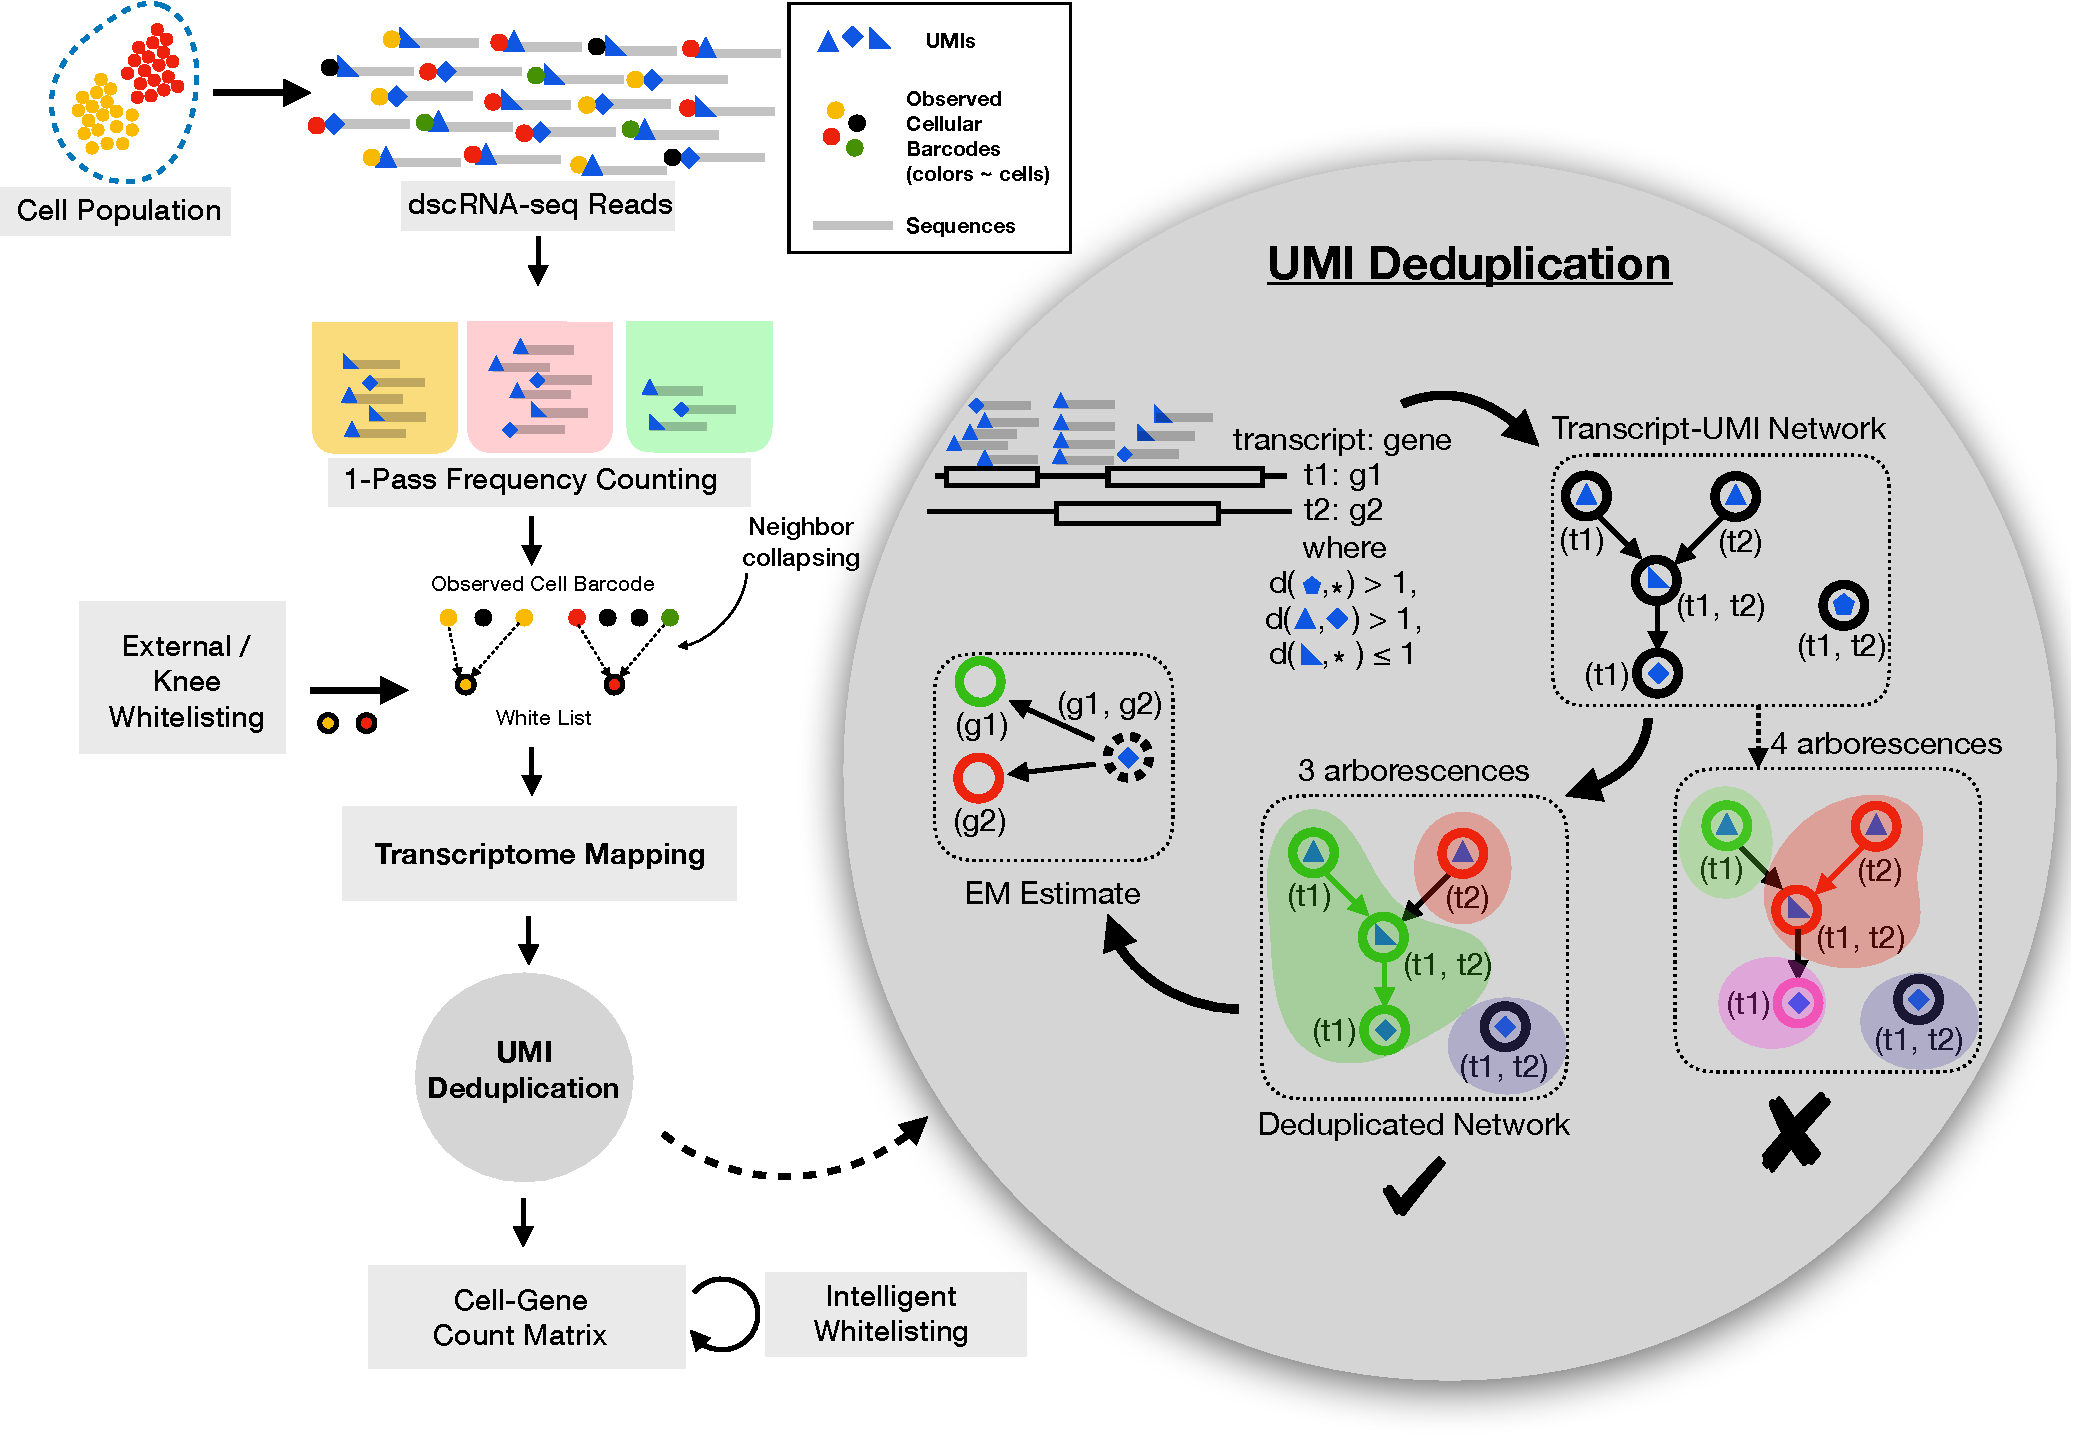
\includegraphics[width=1\textwidth]{alevin/alevin.pdf}
\caption{Overview of the \alevin pipeline. The input to the pipeline are sample-demultiplexed \texttt{FASTQ} files and there are several steps, outlined here, that are required to process this data and obtain per cell gene-level quantification estimates. The first step is cell-barcode (CB) whitelisting using their frequencies. Barcodes neighboring whitelisted barcodes are then associated with (collapsed into) their whitelisted counterparts. Reads from whitelisted CBs are mapped to the transcriptome and the UMI-transcript equivalence classes are generated. Each equivalence class contains a set of transcripts, the UMIs that are associated with the reads that map to each class and the read count for each UMI. This information is used to construct a parsimonious UMI graph (PUG) where each node represents a UMI-transcript equivalence class and nodes are connected based on the associated read counts. The UMI deduplication algorithm then attempts to find a minimal set of transcripts that cover the graph (where each consistently-labeled connected component --- each monochromatic arborescence --- is associated with a distinct pre-PCR molecule). In this way, each node is assigned a transcript label, and in turn, an associated gene label. Reads associated with arborescences that could be consistently labeled by multiple genes are divided amongst these possible loci probabilistically based on an expectation-maximization algorithm. Finally, optionally, and if not provided with high quality CB whitelist externally, an intelligent whitelisting procedure finalizes a list of high quality CBs using a na\"ive Bayes classifier to differentiate between high and low-quality cells.}
\label{fig:pipeline}
\end{figure*}

The process of deduplication requires identifying duplicate reads based on their UMIs and alignment positions along the transcriptome. \Alevin uses a novel algorithm for deduplication that begins by constructing parsimonious UMI graphs, that we refer to as a PUGs, using information from the UMI sequences, the UMI counts and the transcript equivalence classes~\citep{mmseq}. This PUG is constructed such that each UMI-transcript equivalence class pair is represented by a node and there exists an edge from a node to any node that could have arisen from an amplified molecule due to sampling the underlying transcript (a single pre-PCR molecule) at a different position, or via a PCR or a sequencing error being introduced into the UMI.  When the direction of ``duplication'' during PCR is clear, a directed edge is added, otherwise a bi-directed edge is placed. An optimal covering of this graph, using the transcripts associated with each node, will give the minimum number of UMIs, along with their counts, required to explain the set of mapped reads. Hence, we have mapped the deduplication problem to that of finding a minimum cardinality covering of a given graph by monochromatic arborescences. Since the decision version of this problem is NP-complete, we propose a greedy algorithm to obtain a minimum cardinality covering of this graph (proof and algorithm detailed under Materials and Methods). Each covering, and the associated UMI, is assigned a set of transcript labels of size $\geq$ 1. After this UMI resolution phase, the remaining ambiguous reads with more than 1 transcript label, are assigned based on an expectation-maximization method~\citep{salmon}. 

Finally, having obtained per-cell gene expression estimates, CB whitelisting is finalized using a na\"ive Bayes classifier to differentiate between high and low-quality cells utilizing a set of features derived from the expression estimates and other diagnostic features~\citep{dropest}. In addition to the gene-by-cell count matrix, \alevin also provides information about the reliability of the abundance estimate computed for each gene in each cell in the form of a \emph{tier} matrix (and, optionally, the summarized variance of bootstrap estimates), which succinctly encodes the quality of the evidence used to derive the corresponding count.

\subsection{Impact of discarding multimapping reads}

\begin{figure*}[!htb]
  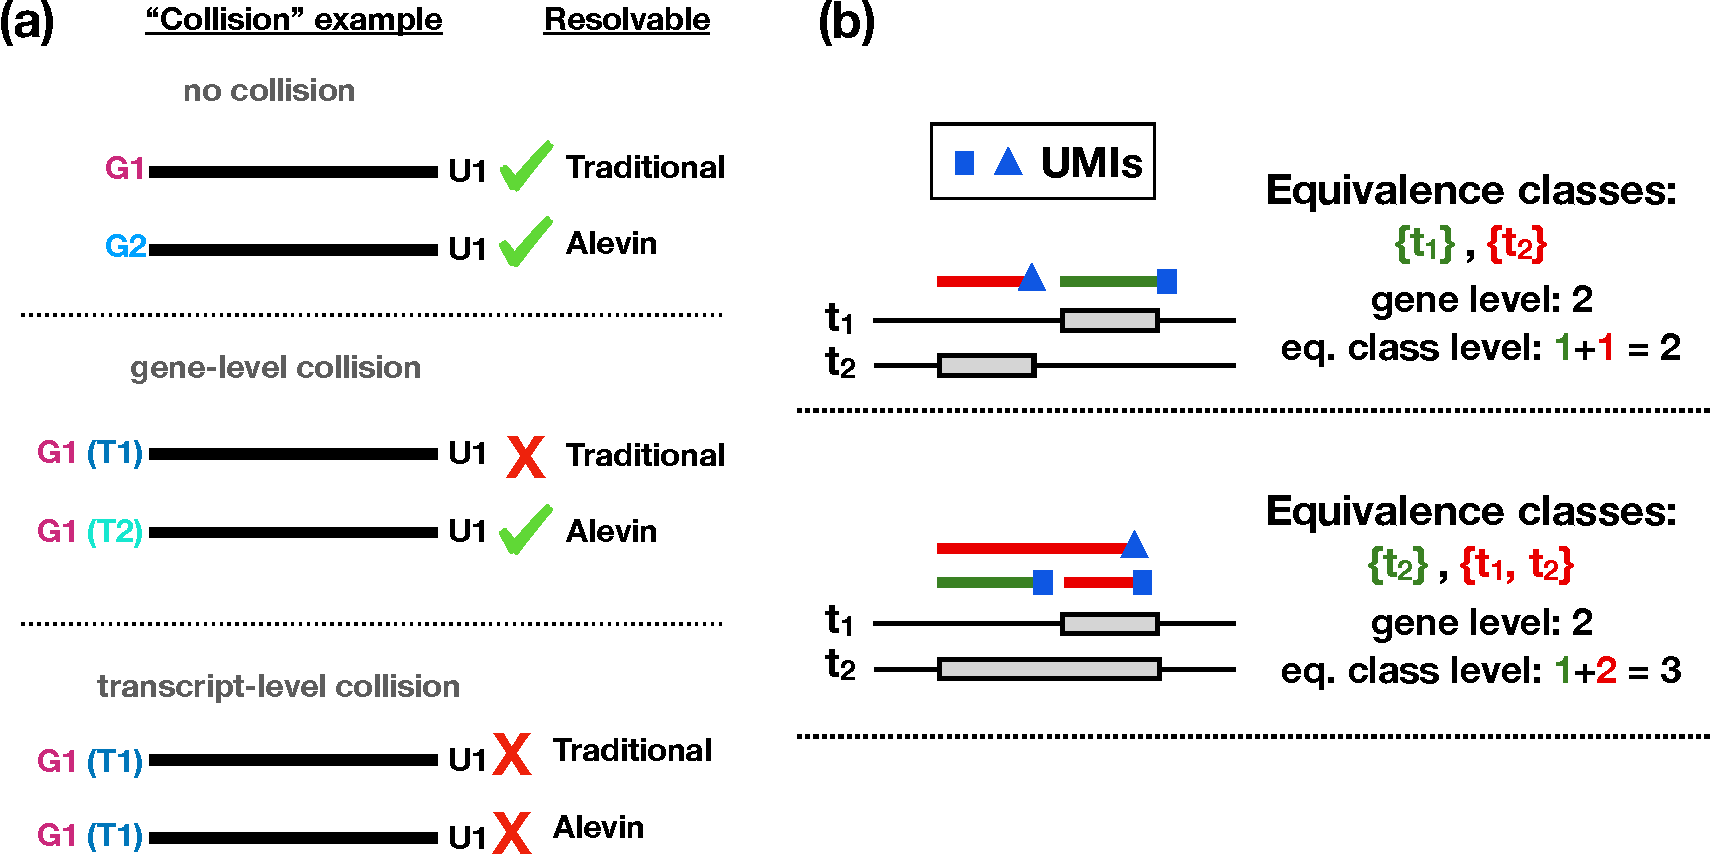
\includegraphics[width=\linewidth]{alevin/sims_combine_final.pdf}
  \caption{(a) This figure illustrates examples of various classes of UMI collisions, and which method(s) would be able to correctly resolve 
  the origin of the multimapping reads in each scenario. These cases are shown top-to-bottom in order of their likelihood. (b) A simulated example demonstrates how treating equivalence classes individually during UMI deduplication can lead 
  to under-collapsing of UMIs compared to gene-level methods (especially in protocols where the majority of cDNA amplification occurs 
  prior to fragmentation). In the first row, both methods report correctly a single UMI. In the second row, there are two fragmented molecules aligned against two transcripts from the same gene. The \alevin deduplication algorithm will attempt to choose the minimum number of transcripts required to explain the read mappings and hence correctly detect the UMI counts. The equivalence class method will over-estimate the gene count.}
  \label{fig:collision_sim}
\end{figure*}

Before proceeding with a more detailed analysis of the \alevin pipeline, it is important to highlight scenarios where existing pipelines would fail using simple examples. These also lead to a better understanding of the \alevin UMI deduplication algorithm that intelligently utilizes transcript-level information to obtain accurate gene-level estimates. 
Since current deduplication methods do not have a mechanism to detect UMIs that map between multiple transcripts of the same gene, they can, in certain cases, incorrectly detect PCR duplicates and hence, under-estimate the total UMI counts. Some obvious cases can be resolved by considering the read-to-transcript mapping, instead of the read-to-gene mapping, as done in \alevin and shown in the left panel in \Cref{fig:collision_sim}.
The first row (top to bottom) demonstrates a case when we observe the same UMI (U1) being used to
tag transcripts from two separate genes (G1 and G2). Here, all methods are able to correctly assess that these instances of U1 are not 
PCR duplicates. In the center row, we observe the same UMI deriving from two (sequence-distinct) transcripts of the same gene. Here,
purely gene-level methods fail to resolve this collision, while \alevin's strategy can. Finally, in the bottom row, we observe a UMI 
collision within a single transcript. That is two different copies (molecules) of the same transcript have been tagged with the same UMI. 
This resolution cannot be resolved by any of the methods.  Though possible, the situation presented in the
third row is \emph{highly}-unlikely, especially given current sequencing depths.

A second scenario is highlighted in the right panel of \Cref{fig:collision_sim}
where using the transcript level equivalence classes lead to over-counting UMIs
(discussed further in Materials and Methods). In these simulated examples, different types of
transcripts, and corresponding expression patterns are shown. 
Reads are randomly sampled from the 3'-end of the
annotated-transcript(s) according to a realistic fragment length distribution,
where exon overlap induces the corresponding equivalence classes of each
fragment. The top simulation shows 1 (pre-PCR) molecule expressed for each transcript, 
identifiable by a unique-id (UMI), shown in blue. Due to the disjoint equivalence classes, both methods will
correctly assign the gene count. In the bottom simulation, both molecules originate from the second transcript. 
However, since the equivalence classes are different, the two fragments sharing a UMI will not be collapsed. 
Specifically, as the rate of splicing (and hence the number of equivalence classes) increases, so too does the number of distinct UMIs 
reported. In this case, the \alevin UMI deduplication algorithm will correctly detect the number of transcripts in order to greedily assign the minimum number of transcripts required to explain the given UMI and mapping information.

\begin{figure*}[!htb]
  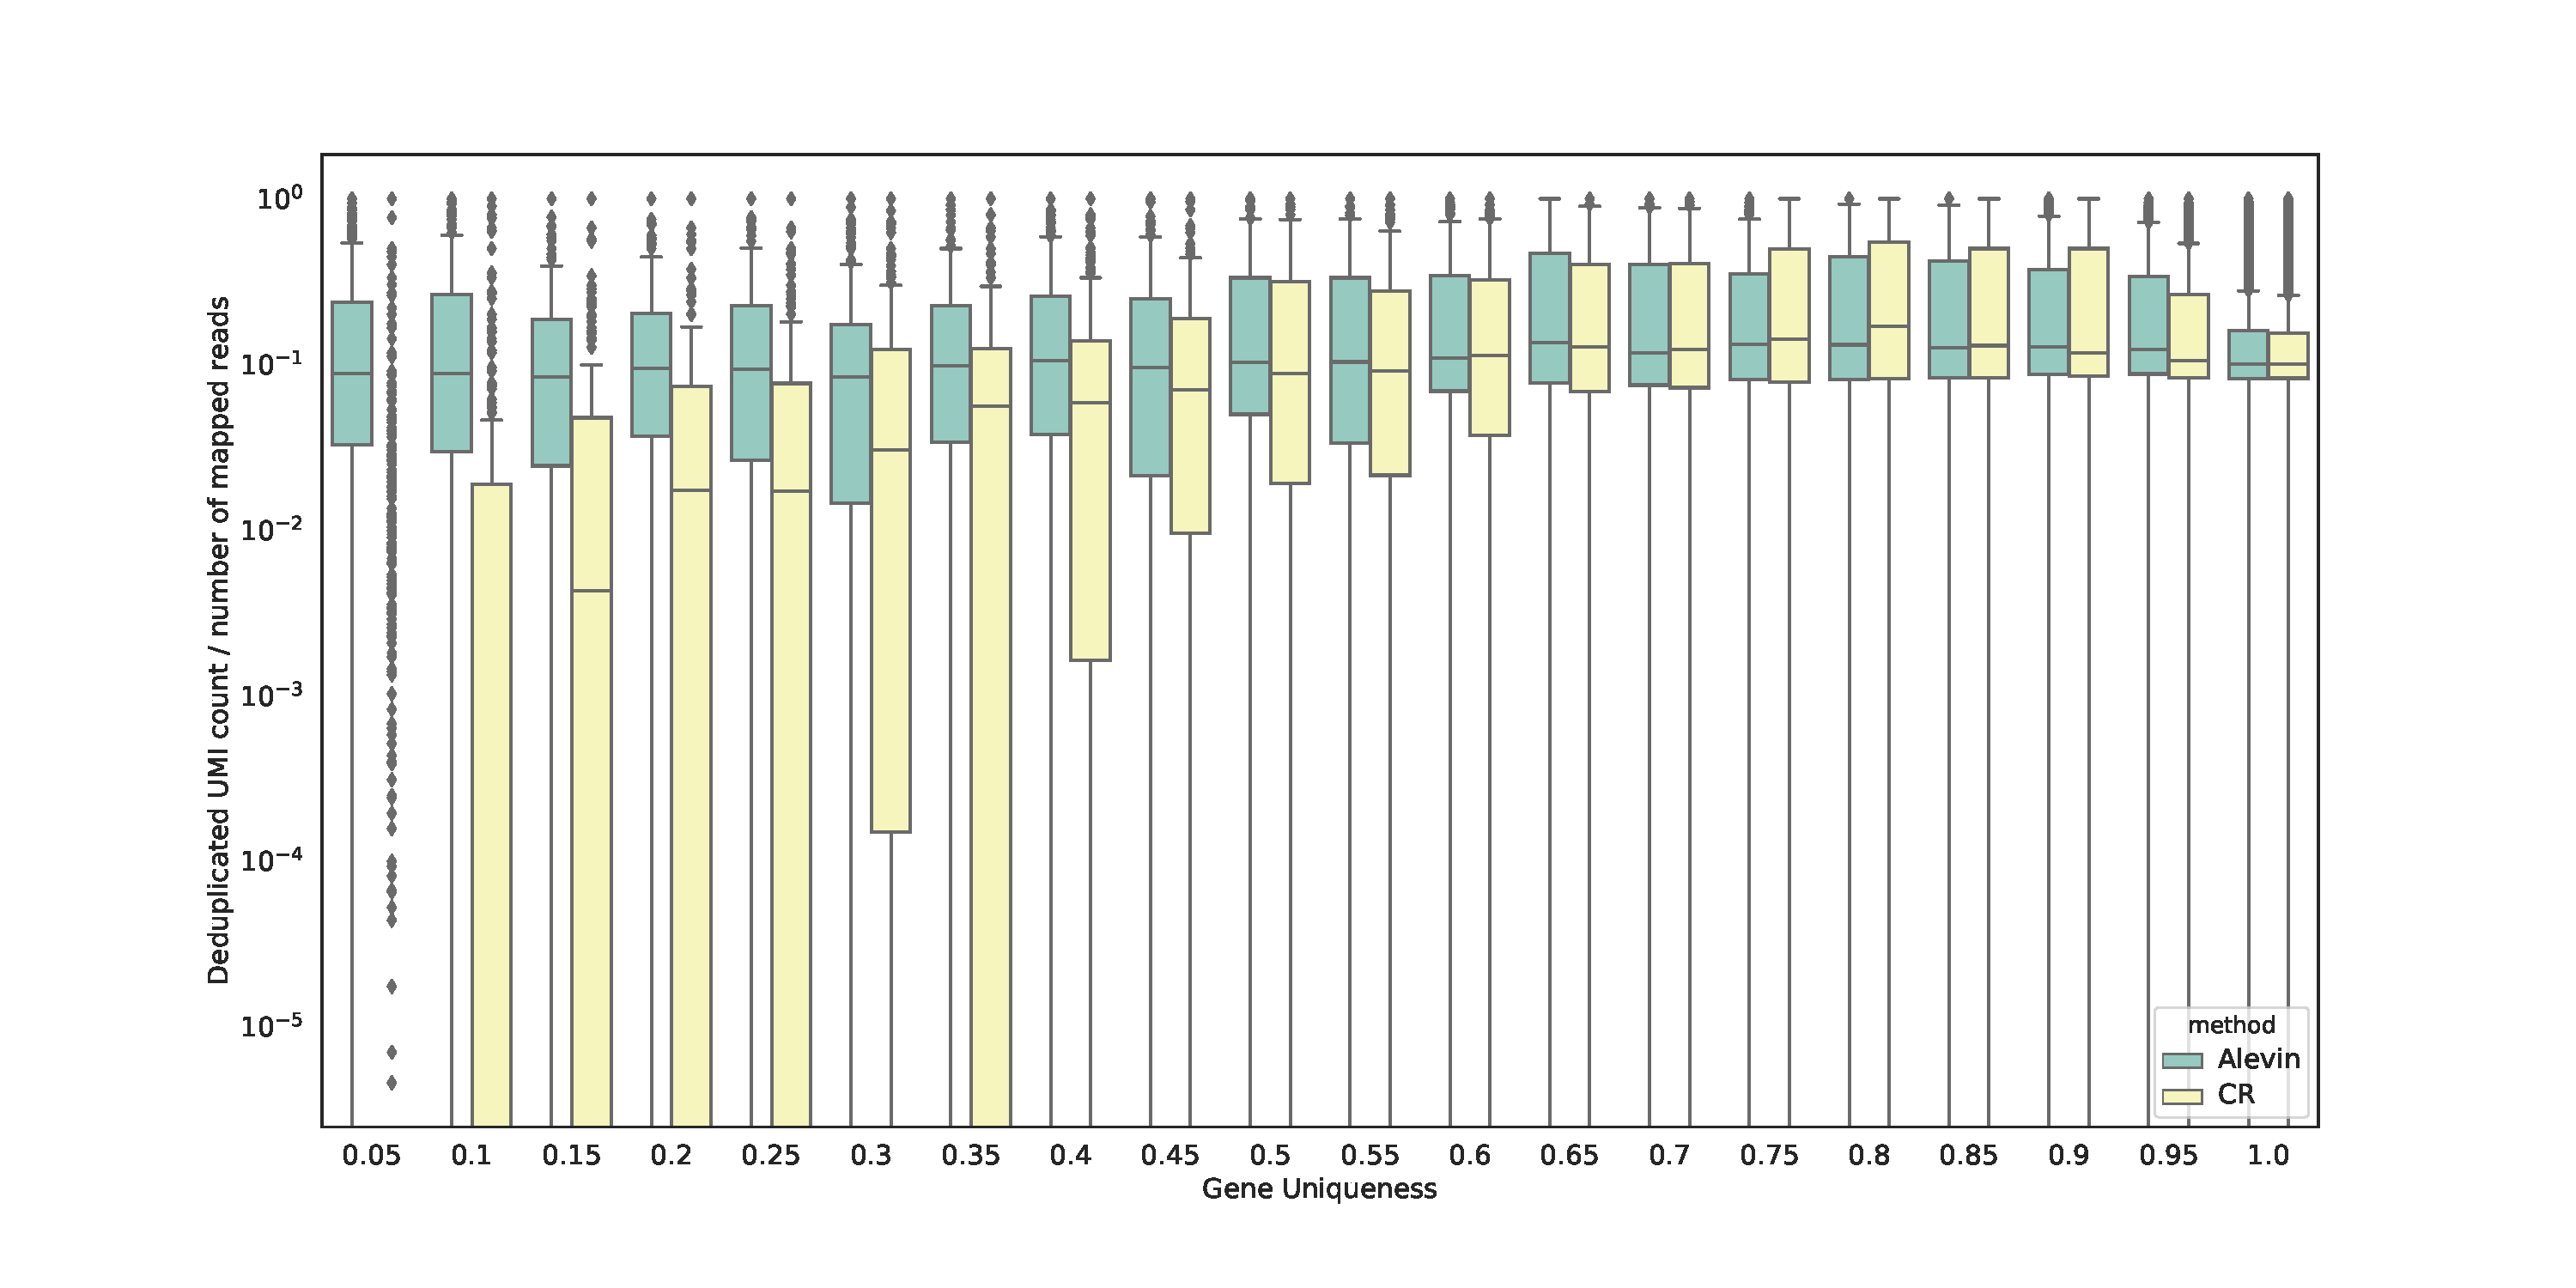
\includegraphics[width=\linewidth]{alevin/UMIdedup.pdf}
  \caption{The ratio of the final number of deduplicated
    UMIs against the number of initial reads for both alevin and Cell Ranger (on the human PBMC 4k dataset)
    stratified by gene-level sequence uniqueness. The genes are divided into
    $20$ equal sized bins and the x-axis represents the maximum gene uniqueness
    in each bin. The plotted ratio for genes that have high sequence
    similarity with other genes is strongly biased when using \cellr. This is
    because \cellr will discard a majority (or all) of the reads originating
    from these genes since they will most likely map to multiple positions
    across various genes. \Alevin, on the other hand, will attempt to accurately
    assign these reads to their gene of origin. This plot also demonstrates that \alevin does not over-count UMIs,
    which would be the case if deduplication was done at the level of equivalence classes.}
  \label{fig:umidedup}
\end{figure*}

To show that the UMI deduplication algorithm from \alevin does, indeed, perform better, we calculate the ratio of the number of reads mapping to each gene and the final count of UMIs as predicted by \alevin and \cellr for that gene. When a read maps ambiguously, the count is divided uniformly between the genes. Hence, if a read maps to two genes, the count for each is incremented by $0.5$ to get the initial number of reads mapping to these genes. Note that the mappings are also different under each pipeline and that some reads may be inherently ambiguous under one or both mappings. These reads cannot be accurately assigned but, while \cellr discards them, \alevin assigns them to a gene via the PUG-resolution algorithm, or,in the case that parsimony fails to distinguish a single best gene, proportionally to multiple genes according to the other uniquely-mapping reads of the experiment.  We divide the genes into 20 bins, based on the number of k-mers shared across genes. We expect the above calculated ratio to remain fairly consistent across these 20 bins, irrespective of the sequence properties of the genes in them. However, we observe in \Cref{fig:umidedup}, that the predictions from \cellr are biased for the genes with low sequence uniqueness. This is because a large number of reads from these genes will multimap across genes and will, therefore, be discarded. Hence, simply discarding multimapping reads seems to bias the count estimates for all genes but strongly impacts counts for genes that are expected to have a larger number of multimapping reads due to their high sequence similarity. 

\subsection{Accuracy analysis on real datasets}
\begin{table}[!htb]
\centering
\caption{Number of final whitelisted cellular barcodes output by \alevin and \cellr.}
      \begin{tabular}{cccc}
        \hline
           Dataset & \cellr  & \Alevin & No.of reads \\ \hline
    Human PBMC 4k & 4346 & 4341 & 379,462,522\\
    Human PBMC 8k & 8379 & 8291 & 784,064,148\\
    Mouse Neurons 900 & 933 & 1291 & 52,805,264 \\
    Mouse Neurons 2k & 2009 & 1881 & 147,010,995 \\
    Mouse Neurons 9k & 9116 & 8519 & 383,366,284 \\ \hline
      \end{tabular}
      \label{suptab:whitelist}
\end{table}

To assess the performance of \alevin, both in terms of accuracy in quantification and resource consumption, we ran it on 10x Chromium datasets from human and mouse. We compare our results against the \cellr pipeline\citep{tenx}, the \dropest pipeline\citep{dropest} \footnote{Note that we were not able to run the dropEstr Bayesian correction method and the results presented are after running just the \dropest pipeline~\cite{dropseqsrc}.}. , and a custom pipeline, with an external list of whitelisted CBs, using STAR\citep{star}, featureCounts \citep{featurecounts}, and UMI-tools \citep{umitools}, which we refer to as the \naive pipeline. The exact parameters for running each tool are provided under Materials and Methods. Note that we run \alevin with the \texttt{{--}keepDuplicates} flag during indexing, which ensures that even when multiple sequence-identical transcripts exist in the annotation, they are not discarded. This is to allow for fair comparison against the other tools, since they do not discard such transcripts, and the existence of such transcripts will impact the number of multimapping reads. However, we do not generally recommended using this flag when running \alevin. We observe that the number of final whitelisted cells predicted by \alevin are in close proximity to the count of cells predicted by \cellr (and \dropest, since they use the same whitelise), but there are non-trivial differences (\Cref{suptab:whitelist}). Comparison on data using the Drop-seq\citep{dropseq} protocol is also detailed below. Comparisons against the recently released version 3.0.0 of \cellr are also provided (Additional file 1: Figure S1), along with results from another run of \alevin using different parameters. Where mentioned, the results are stratified by gene uniqueness which is the proportion of k-mers, of size 31, that are not shared between two or more genes. We note that varying the k-mer size changes the stratification of the genes but does not impact the overall correlation and performance of the methods. We show this for the mouse neuronal 900 dataset (Additional file 1: Figure S2). We calculated this for each gene in the human (GENCODE release 27, GRCh38.p10) and mouse (GENCODE release M16, GRCm38.p5) transcriptomes. Note that this was not calculated using the canonicalized k-mers from the genes. This is because the \scrnaseq protocols are stranded and a read, therefore, can not multi-map between two genes if the reverse complement of one of them is shared with the other's forward sequence. 

\subsection{Accuracy of estimates against bulk data}
\begin{table}[!htb]
\centering
\caption{Average Spearman correlation of gene-level estimates from each method for the single cell datasets against bulk data from the same cell types (4 for human, 3 for mouse).}
      \begin{tabular}{ccccc}
        \hline
           Dataset & \Alevin & \cellr & \naive & DropEst \\ \hline
           Human PBMC 4k & 0.813 & 0.780 & 0.747 & 0.783 \\
           Human PBMC 8k & 0.810 & 0.772 & 0.740 & 0.776 \\
           Mouse Neurons 900 & 0.812 & 0.773 & 0.761 & 0.779 \\
           Mouse Neurons 2k & 0.822 & 0.781 & 0.767 & 0.784\\
           Mouse Neurons 9k & 0.831 & 0.796 & 0.776 & 0.803 \\ \hline
      \end{tabular}
      \label{suptab:fullcorr}
\end{table}

To test the accuracy of the quantification estimates, we aggregate the estimates from each of the single-cell quantification tools (summing across all cells) and calculate the correlation with estimates predicted by RSEM\citep{li2011rsem} (paired with Bowite2\citep{bowtie2} alignments) using bulk datasets from the same cell types. While the differences between single-cell and bulk sequencing protocols and techniques are significant, we believe that, in the absence of established benchmarks, the correlation between them is a reasonable indicator of the accuracy of each quantification method. Estimates from \alevin, when summed across all cells, have a higher Spearman rank correlation than the \cellr, \dropest, and \naive pipelines (\Cref{suptab:fullcorr}).  Specifically, we posit that the methods demonstrate a strong and persistent bias against groups of two or more genes that exhibit high sequence similarity.  That is, the more sequence-similar a gene is to another gene, the less likely these pipelines are able to assign reads to it --- in the extreme case, some genes essentially become \emph{invisible} due to the \emph{in silico} biases of these approaches (a similar effect was reported by Robert and Watson ~\citep{makemickhappy} in bulk RNA-seq data when simple read-counting approaches are used for quantification, where they highlight that many such genes are relevant to human disease).

\begin{figure*}
\centering
    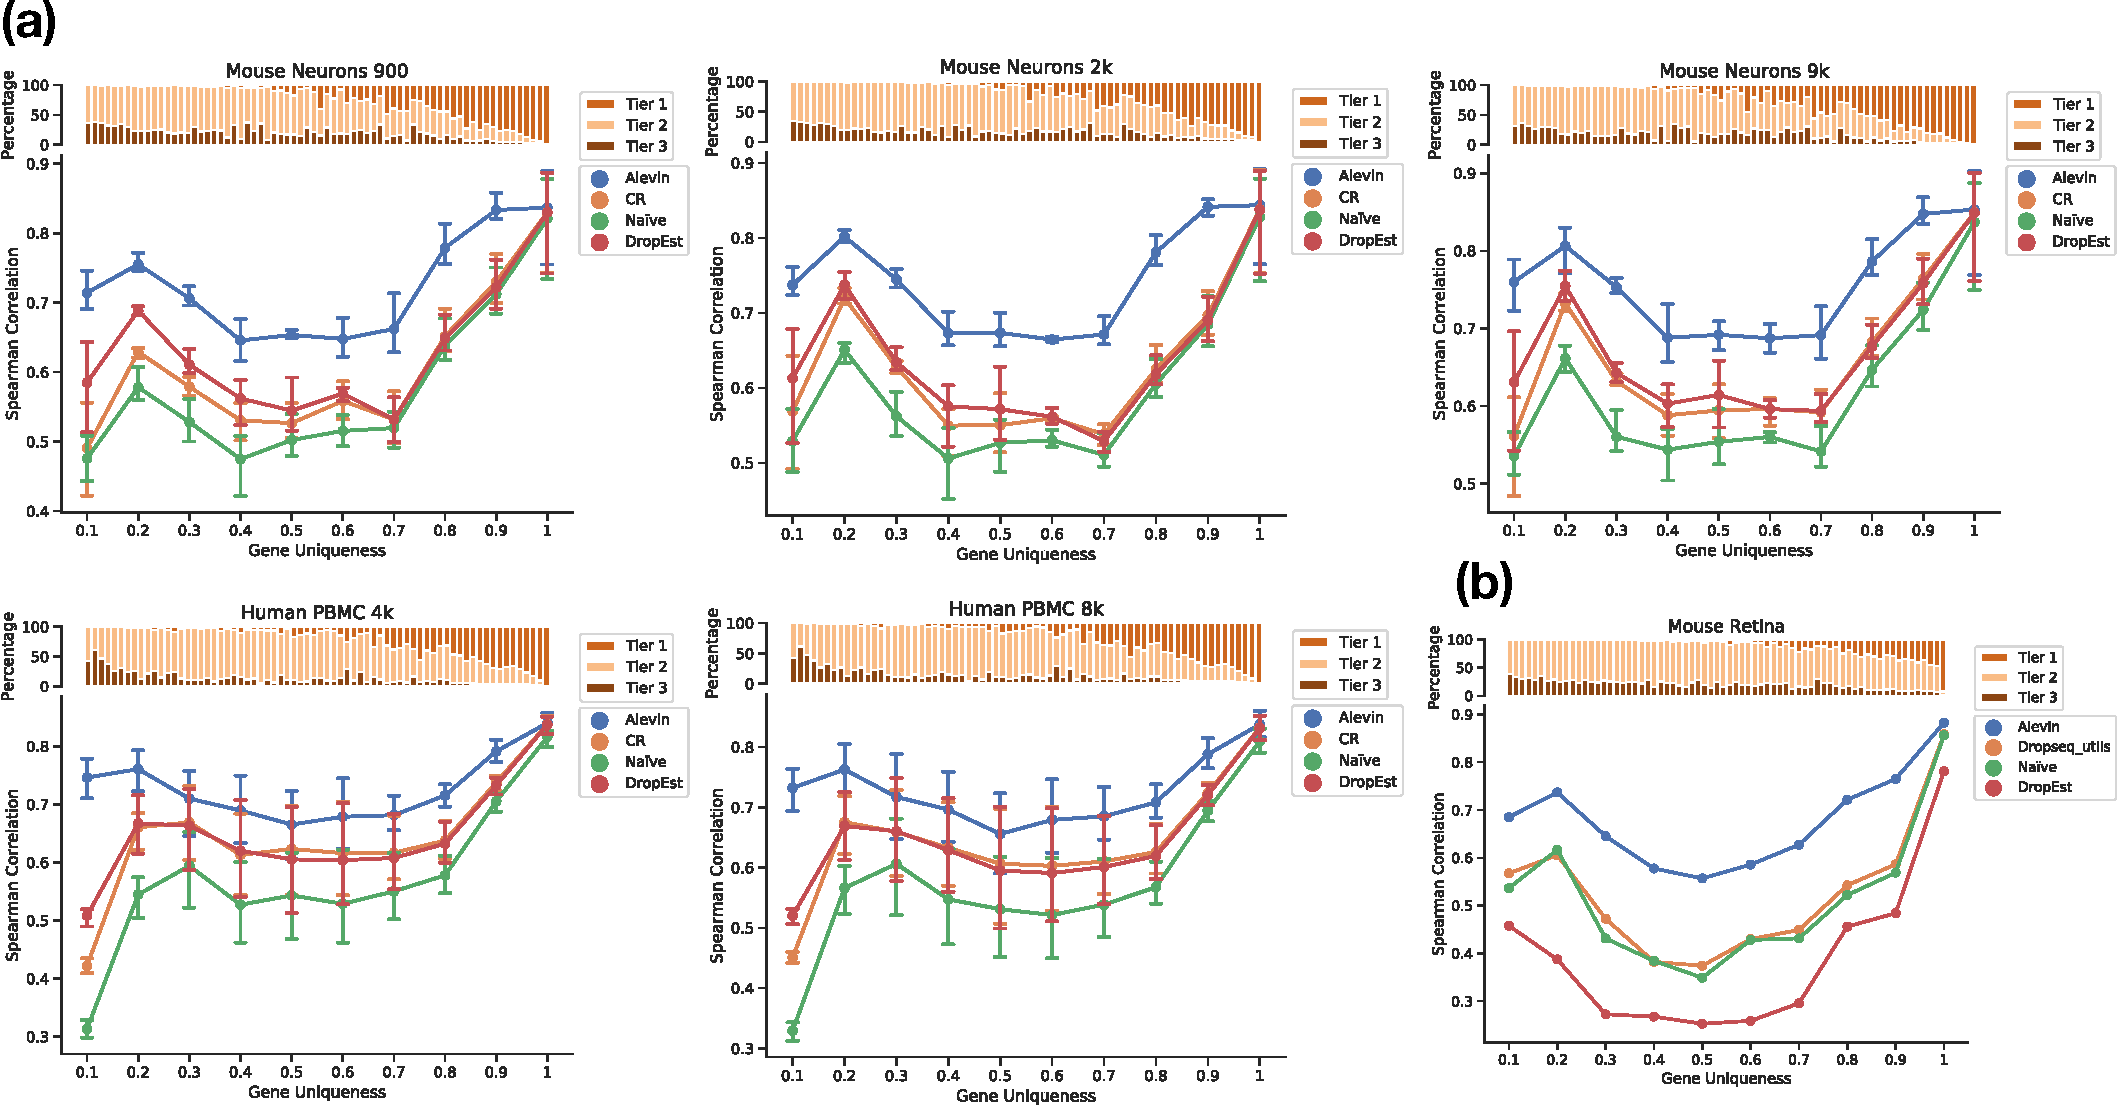
\includegraphics[width=\linewidth]{alevin/combine_corr.pdf}
  \caption{(a) The Spearman correlation between quantification estimates (summed across all cells) from different \scrnaseq methods against bulk data from the mouse neuronal and human PBMC datasets, stratified by gene sequence uniqueness. The bar plot on the top of each figure shows the percentage of genes in each bin that have unique read evidence. Tier 1 is the set of genes with only uniquely mapping reads. Tier 2 is genes that have ambiguously mapping reads, but are connected to unique read evidence that can be used to resolve the multimapping reads. Tier 3 is  genes that are completely ambiguous. Note that all methods perform very similarly on genes from tier 1, but the performance of \alevin is much better for the other tiers. (b) Comparison of various methods used to process dropseq data from mouse retina with 4k cells. The Spearman correlation is calculated against bulk quantification estimates predicted using Bowtie2 and RSEM on data from the same cell type.}
  \label{fig:correlation}
\end{figure*}

\begin{table}[!htb]
\centering
\caption{Number of genes in each bin, when stratified by gene uniqueness.}
      \begin{tabular}{ccc}
        \hline
           Bin number & Human  & Mouse \\ \hline
    1 & 3155 & 4786 \\
    2 & 894 & 1089 \\
    3 & 853 & 945 \\
    4 & 822 & 1061 \\
    5 & 962 & 1104 \\
    6 & 1174 & 1318 \\
    7 & 1565 & 1476 \\     
    8 & 2546 & 1877 \\ 
    9 & 4695 & 2960 \\ 
    10 & 41622 & 36763 \\ \hline
      \end{tabular}
      \label{suptab:bin_sizes}
\end{table}

To further explore this hypothesis, we stratified the accuracy of the different methods by the uniqueness of the underlying genes (\Cref{fig:correlation}a, \Cref{suptab:bin_sizes}). The bar plots at the top of each subfigure represent the tiers of the genes as assigned by \alevin. Tier 1 is the set of genes where all the reads are uniquely mapping. Tier 2 is genes that have ambiguously mapping reads, but connected to unique read evidence as well, that can be used by the EM to resolve the multimapping reads. Tier 3 is the genes that have no unique evidence and the read counts are, therefore, distributed between these genes according to an uninformative prior. In agreement with the hypothesized relationship, we observed that the higher accuracy of \alevin is particularly large for genes with a lower proportion of unique k-mers, that tend to belong to tier 2 or 3. On genes from tier 1, all the methods to perform similarly. Thus, the approach of \cellr, \dropest, and \naive, which discard reads mapping to multiple genes, results in systematic inaccuracies in genes which are insufficiently unique (i.e. which share a high degree of sequence homology with some other gene). 

\begin{figure*}[!htb]
  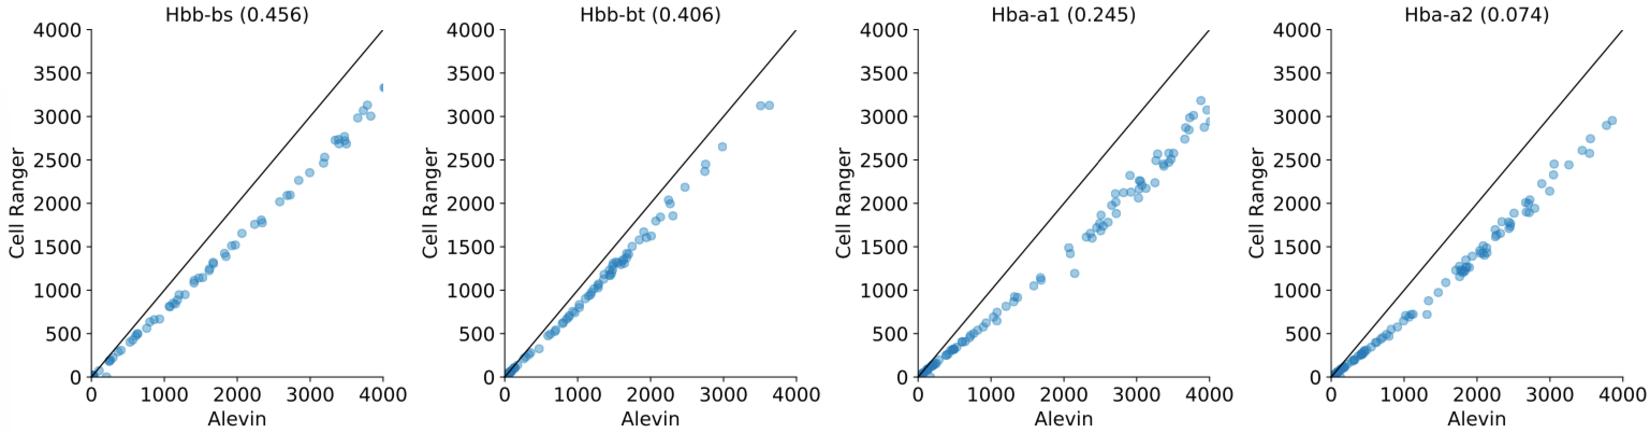
\includegraphics[width=\linewidth]{alevin/hbgene.pdf}
  \caption{Expression of the Hba and Hbb genes as predicted by \alevin and \cellr in mouse neuronal cells. The title of each plot is the name of the gene and its k-mer uniqueness ratio. Note that \cellr systematically underestimates the expression of these genes compared to \alevin. This bias is greater for the Hba genes, which have a lower uniqueness ratio, and therefore, a greater number of multi-mapping reads.}
  \label{fig:hbgene}
\end{figure*}

\begin{figure}[!htb]
    \centering
  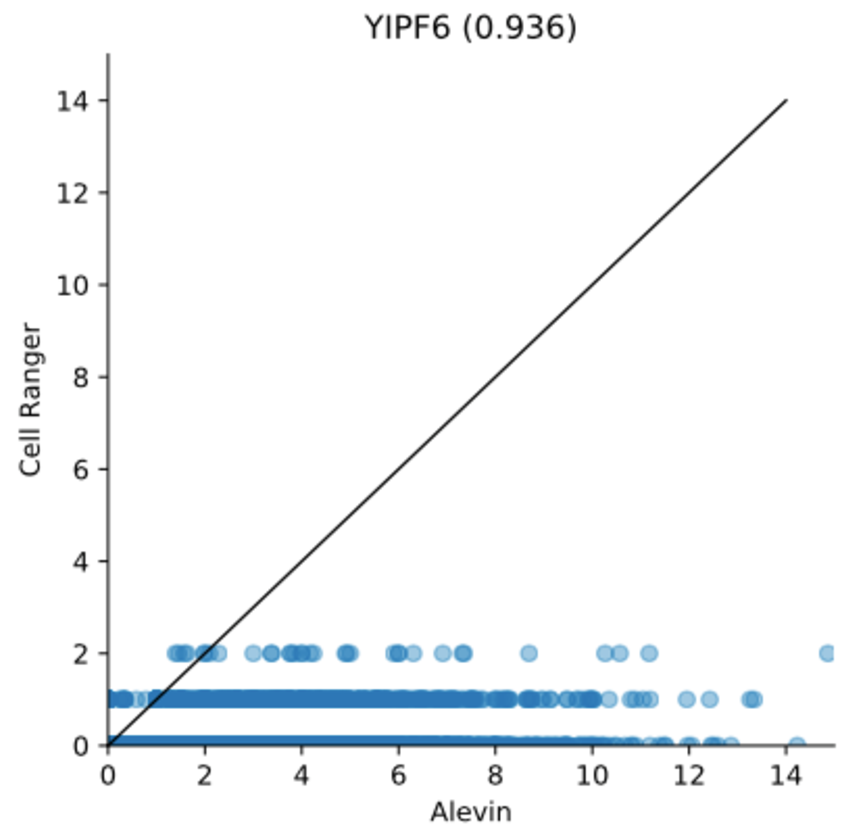
\includegraphics[width=0.3\linewidth]{alevin/yipf6gene.pdf}
  \caption{Expression of the YIPF6 gene (which has a high uniqueness ratio) as predicted by \alevin and \cellr in the PBMC8k data.}
  \label{fig:yipgene}
\end{figure}

This bias could impact the expression estimates of important marker genes, such as the genes for the hemoglobin alpha and beta proteins in the mouse neurons\citep{han2018mapping, richter2009neurons}. Due to their lower uniqueness ratio, \cellr appears to exhibit a bias against such genes, and their expression, as predicted by \alevin, is systematically higher (\Cref{fig:hbgene}).  Anecdotally, we also noticed that, in the human PBMC data, \alevin sometimes predicts the expression of even relatively sequence-unique genes, like YIPF6, that we expect to be expressed in a subpopulation of these cells (monocytes)~\citep{yipf6}, but which exhibit almost no expression as predicted by \cellr (\Cref{fig:yipgene}).  Because the bias against sequence-ambiguous genes is fundamental and sequence-specific, it cannot be easily remedied with more data, but instead requires the development of fundamentally novel algorithms, like \alevin, that account for, rather than discard, reads mapping to such genes. Hence, \alevin not only quantifies a greater proportion of the sequenced data than existing methods, but also does so more accurately and in a less-biased manner.

\subsection{Accuracy of estimates using combined genomes}
To further assess the accuracy of quantification estimates, in the absence of
  any established read-level simulation protocol, we performed an experiment aimed
  to introduce controlled gene-level multimapping to analyze its effect on the
  different methods.  We quantified the mouse neuronal 900 sequencing dataset
  using both \cellr and \alevin and each quantification was performed under
  two separate references: the mouse genome, and the combined human and mouse genome.
  Noting that the reads in this experiment originate from mouse, we
  desire that the quantifications returned by a method deviate as little as
  possible under the two different reference configurations. Under ideal
  conditions, for example, the gene counts under both references should be the
  same. However, combining the mouse and human references increases the gene
  sequence ambiguity, due to the presence of homologous genes, resulting in
  misestimation. 
  
  \begin{figure}[!htb]
      \centering
    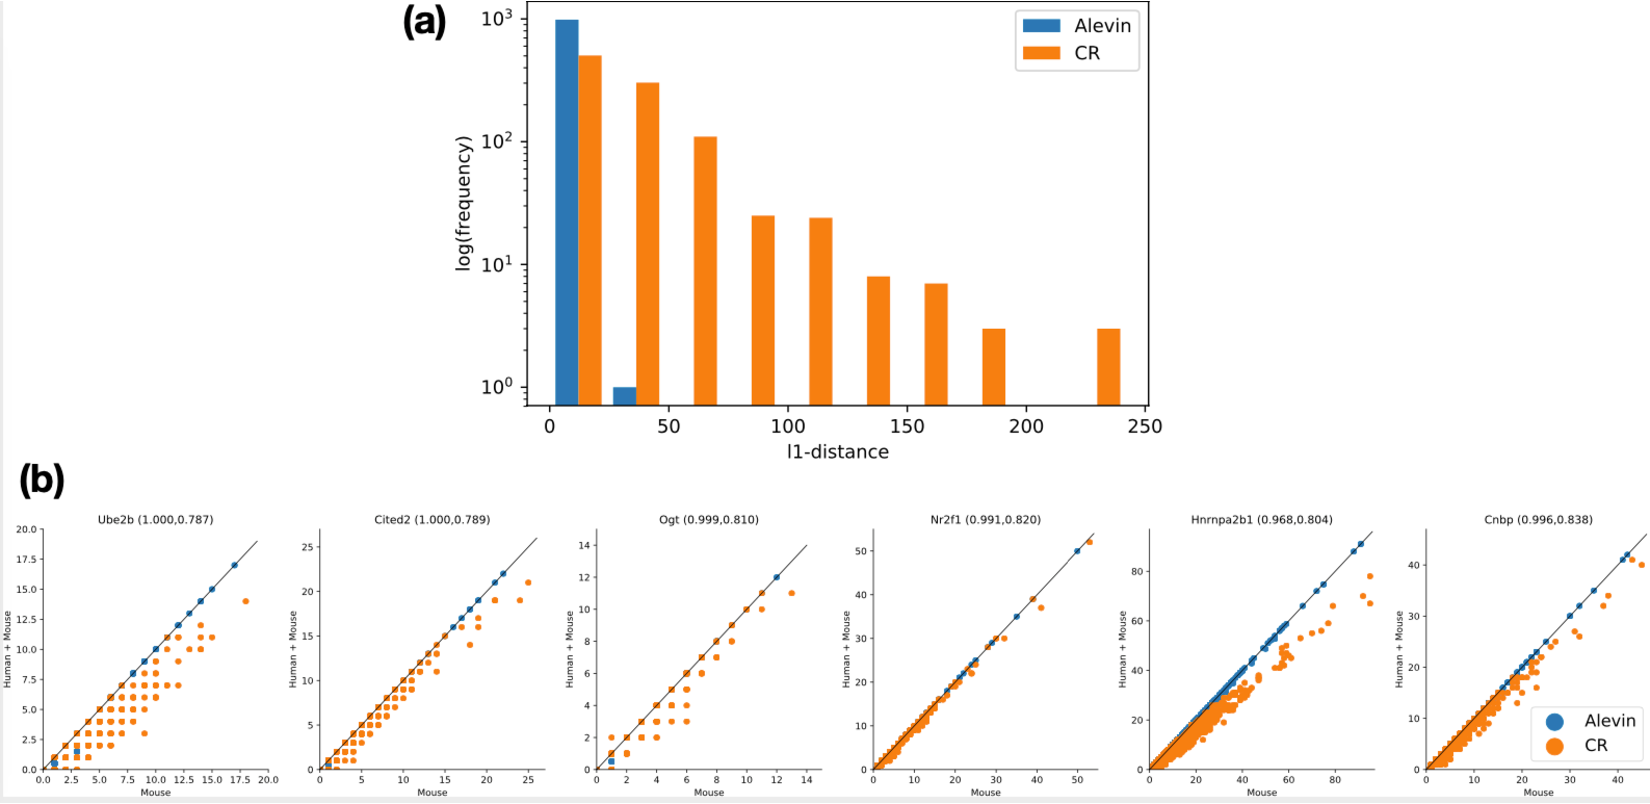
\includegraphics[width=\linewidth]{alevin/mixed_combine.pdf}
    \caption{(a) Histogram of the $\ell_{1}$ distance between the
        quantification estimates of tools on the mouse neuron 900 data, when run
        using different references for quantification (just mouse versus mouse and
        human). Results are presented for both \alevin and \cellr. Since, in
        reality, all reads are expected to originate from mouse, deviations from
        quantifications under the only mouse reference signify misestimation ---
        often due to the introduction of sequence-similar genes in the human
        genome. Alevin is able to resolve this ambiguity well, while \cellr
        instead discards such reads, leading to different quantification estimates
        under the two references. (b) Counts for the topmost genes that have high sequence homology between human 
        and mouse but are sequence unique in the mouse reference. The title of each plot is the gene name 
        along with the sequence uniqueness ratio under just the mouse reference and under the joint reference. Hence, the
        \cellr counts decrease across cells when the gene uniqueness decreases. Note that these genes were filtered such
        that they have $>$100 count difference for either \alevin or \cellr when summed across all cells. }
    \label{fig:mixedanalysis}
  \end{figure}
  
  We show in \Cref{fig:mixedanalysis}a that the distance under
  the two references is higher for the \cellr estimates than that for the
  \alevin estimates. Due to the increased homology among genes between the
  references, the ratio of reads mapping to multiple genes increases, resulting
  in more information being discarded by \cellr. The total number of UMIs
  accounted for by \cellr decreases by $\sim20,000$, in comparison the number of
  distinct UMIs predicted by \alevin decreased by $\sim1,500$, which one might
  attribute to changes in the underlying PUGs as a result of mapping
  $\sim0.01\%$ more reads. The number of human genes expressed (non-zero UMI count)
  under the joint reference is $624$ for \cellr and $600$ for \alevin, out of a total of $58,288$ genes. 
  Note that in both cases, these genes account for $<0.05\%$ of the total UMI count predicted by each 
  method.

  To provide a statistical analysis of the differences observed for the methods
  under the two different reference sequences, we performed the following test.
  We sample, randomly, $1000$ sets of $100$ cells from the entire experiment,
  and for each sample, we compute the sum of absolute difference between the
  predictions of each tool under both references. We compare the resulting
  distribution of differences for \cellr with that of \alevin and find that the
  differences in \alevin's quantifications are smaller than those of \cellr ($p < 0.001$, Mann Whitney Wilcoxon test). 
  These distributions are plotted in Additional file 1: Figure S3.

 We also show in \Cref{fig:mixedanalysis}b that, for the genes that have
  sequence similarity in the joint reference but are unique in the mouse genome,
  \cellr expression estimates vary much more than those from \alevin.

\subsection{Time and memory efficiency}
The time and memory requirements for \alevin are significantly less than those for the existing pipelines (\Cref{fig:timemem}), where all methods were run using $16$ threads. DropEst is excluded from the figure since it consumes the BAM file output by \cellr and is not a complete end-to-end pipeline. For the smallest dataset (900 mouse neuronal cells), \alevin was $\sim5$ times faster than \naive and $\sim21$ times faster than \cellr. This difference increases further as the size of the dataset increases, since the performance of \alevin scales better than the other tools. Hence, where \alevin took only $70$ minutes to process the human PBMC 8k dataset, \cellr took $22$ hours and \naive took $11$ hours. On this dataset, \dropest took $\sim2$ hours, after \cellr was used to process and align the reads. In terms of memory, \alevin used only $\sim13$GB on the human PBMC 8k cell dataset, whereas \naive took $\sim20$GB and \dropest took $\sim32$GB. For the mouse neuronal 9k cell dataset, \alevin used $\sim14$GB, \naive  $\sim18$GB, and \dropest $\sim52$GB. In both cases, \cellr required a minimum of 16GB just for STAR indexing. We note that \cellr allows the user to specify a maximum resident memory limit, and we ran \cellr allowing it to allocate up to 120GB so that the extra runtime was not due to limitations in available memory. We also note that for \dropest, we were not able to run the Bayesian collision correction algorithm implemented in dropEstr; however, given the relatively long UMI tags employed in chromium V2 chemistry compared to inDrop, one would expect the effect of this extra phase to be limited anyway.

\begin{figure*}[!htb]
    \centering
  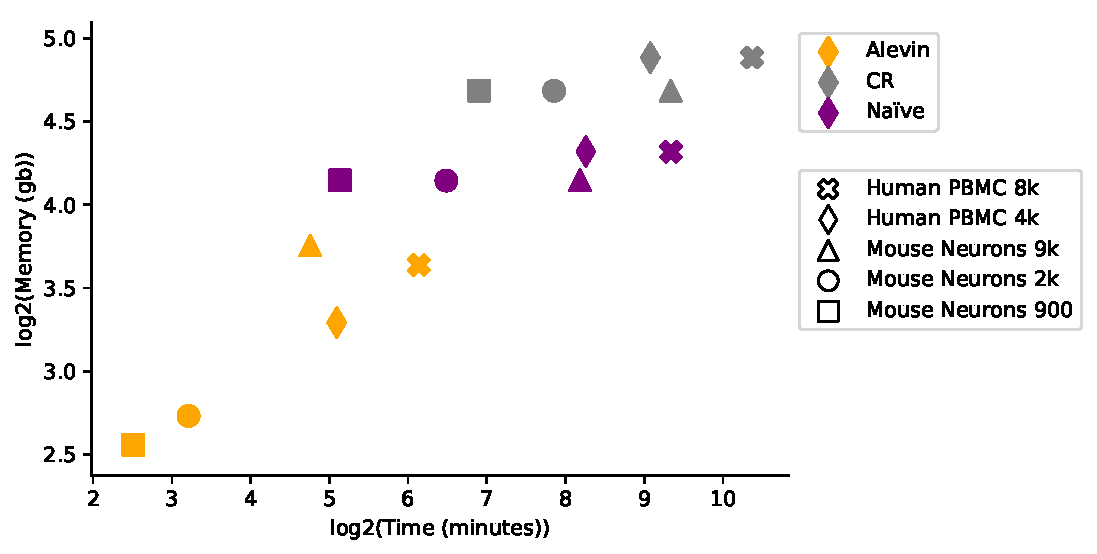
\includegraphics[width=\linewidth]{alevin/timing.pdf}
  \caption{The time and memory performance of the different pipelines on the five datasets. \Alevin requires significantly less time and memory than the other pipelines. Note that for \cellr, the memory plotted is the lower bound, which is the size of the index and the actual memory usage can be much higher.} %(b) The time and memory usage of \alevin using different number of threads. The runs for each dataset were repeated using $5, 10, 15,$ and, $20$ threads.}
  \label{fig:timemem}
\end{figure*}

We observe that the optimal number of threads for running \alevin is $10-12$, where the maximum gain in terms of time and memory is achieved. \Alevin is designed to make efficient use of multiple threads, though the optimal number of threads can depend on many factors, such as the speed of the underlying disk and the size of the raw input and output matrix to be written. While runtime decreases with the number of threads uses, the memory profile changes very little as threads are added. 

\subsection{Comparison on DropSeq data}
In addition to data generated using the 10x chromium protocol\cite{tenx}, we 
also tested \alevin on mouse retina data generated using the Drop-seq protocol~\citep{dropseq}. 
We compare \alevin against UMI-tools (the \naive pipeline    
from the main paper), \dropest, and dropseq\_utils~\citep{dropseq} --- the processing    
pipeline originally used by~\citet{dropseq}.   
 Again, we compared the correlation of gene abundances, summed across all cells    
and as produced by the different methods with the estimates from bulk    
data~\citep{mouse_retina} in the same tissue (\Cref{fig:correlation}b). We observe a    
similar trend across gene-uniqueness bins as was observed for the 10x datasets.    
\Alevin demonstrates higher correlation, overall, with the bulk data, and the    
improvements are particularly substantial for genes that are not    
sequence-unique. Further, \alevin is much faster, and takes less memory than    
the other pipelines. \Alevin took $17$ minutes to process this data, which is much faster than the UMI-tools-based    
pipeline ($\sim3.2$ hours), the dropseq\_utils-based pipeline ($\sim15.5$    
hours), and even \dropest ($25$ minutes). The memory usage of \alevin was $6.5$GB, which is less than half the    
memory usage of the closest tool (UMI-tools at $17.72$GB).
The dropseq\_utils-based pipeline took $25.07$GB and while \dropest used
$10.8$GB, that does not include the memory consumed by \cellr to index the reference and align reads against it to
produce the BAM file.
While \alevin has been primarily designed and tested with 10x data in mind, the method
is generic for droplet-based tagged-end protocols, and we observe that it also seems to perform
well on Drop-seq data. 

\section{Conclusion}
We present a new end-to-end pipeline for performing gene-level quantification
from \dscrnaseq that is accurate, efficient, and easy to use. Our method,
\Alevin, relies on a new formulation of the UMI-resolution problem that both
accounts for transcript-level constraints on how UMIs may have been generated
and that allows resolving the potential origin of a UMI even when the
corresponding reads map between multiple genes.

Our analyses demonstrate that, compared to \cellr (and \naive), \alevin achieves
a higher accuracy, in part because of considering a substantially larger number
of reads. Further, \alevin is considerably faster and uses less memory than
these other approaches. These speed improvements are due to a combination of the
fact that \alevin uses bespoke algorithms for CB and UMI edit distance
computation, read mapping, and other tasks, and is a unified tool for performing
all of the initial processing steps, obviating the need to read and write large
intermediate files on disk. These optimizations make it possible to efficiently
process \dscrnaseq datasets on commodity computers reducing computational
barriers to processing and re-processing of such data.

In the future, we hope to further improve the benchmarking of accuracy
  for single-cell quantification and barcode whitelisting approaches, as the
  lack of standard benchmarks makes the assessment of new methods difficult. We
  also hope to explore alternative cell barcode whitelisting and PUG resolution strategies --- for example,
  adopting a generative model for PCR and sequencing error and seeking a maximum
  likelihood rather than maximum parsimony-based resolution of the PUGs.


% Chapter 1

\chapter{Conclusion and Future Work} % Main chapter title

\label{conclusion} % For referencing the chapter elsewhere, use \ref{Chapter1} 

%----------------------------------------------------------------------------------------

% Define some commands to keep the formatting separated from the content 
% \newcommand{\keyword}[1]{\textbf{#1}}
% \newcommand{\tabhead}[1]{\textbf{#1}}
% \newcommand{\code}[1]{\texttt{#1}}
% \newcommand{\file}[1]{\texttt{\bfseries#1}}
% \newcommand{\option}[1]{\texttt{\itshape#1}}

\section{Discussion \& Conclusion}

In this study, we have argued for the usefulness of our novel approach, \qm, for mapping RNA-seq reads.  More generally, we suspect that read \textit{mapping}, wherein sequencing reads are assigned to reference locations, but base-to-base alignments are not computed, is a broadly useful tool.  The speed of traditional aligners like \bt and \STAR is limited by the fact that they must produce optimal alignments for each location to which a read is reported to align.

In addition to showing the speed and accuracy of \qm directly, we apply it to a problem in transcriptome analysis. we have updated the Sailfish software to make use of the \qm information produced by \rapmap, rather than direct \kmer counts, for purposes of transcript-level abundance estimation.  This update improves both the speed and accuracy of Sailfish, and also reduces the complexity of its code base. We demonstrate, on synthetic data generated via two different simulators, that the resulting quantification estimates have accuracy comparable to state-of-the-art tools. 

However, \rapmap is a stand-alone mapping program and need not be used only for the applications we describe here.  We expect that \qm will prove a useful and rapid alternative to alignment for tasks ranging from filtering large read sets (e.g. to check for contaminants or the presence or absence specific targets) to more mundane tasks like quality control and, perhaps, even to related tasks like metagenomic and metatranscriptomic classification and abundance estimation. We hope that the \qm concept, and the availability of \rapmap and the efficient and accurate mapping algorithms it exposes, will encourage the community to explore replacing alignment with mapping in the numerous scenarios where traditional alignment information is unnecessary for downstream analysis.

\section{Future Work}

The concept of \qm is fast, accurate and solves an important problem, read-mapping. Since the mapping approach is still new and unexplored, we are reaching out to find other biological applications where \rapmap can be useful. In the following section, we discuss some of the applications on which we are currently working. However, this is in no way an exhaustive list and we believe \rapmap has the capability to simplify many more biological analysis.

\subsection{RapClust~\citep{srivastava2016accurate}}

Estimating gene expression from RNA-seq reads is an especially challenging task when no reference genome is present. Typically, this problem is solved by performing \denovo assembly of the RNA-seq reads, and subsequently mapping these reads to the resulting contigs to estimate expression. Due to sequencing errors and artifacts, and genetic variation and repeats, \denovo assemblers often fragment individual isoforms into separately assembled contigs.  \citet{corset} argue that better differential expression results can be obtained in \denovo assemblies if contigs are first clustered into groups.  They present a tool, CORSET, to perform this clustering, and compare their approach to existing tools such as CD-HIT~\citep{fu2012cd}. CD-HIT compares the sequences (contigs) directly and clusters them by sequence similarity. CORSET, alternatively, aligns reads to contigs (allowing multi-mapping) and defines a distance between each pair of contigs based on the number of multi-mapping reads shared between them, and the changes in estimated expression inferred for these contigs under different conditions. Hierarchical agglomerative clustering is then performed on these distances to obtain a clustering of contigs.

\rapmap can be used for the same task, by taking an approach similar to that of CORSET. By mapping the RNA-seq reads to the target contigs and simultaneously constructing collapsed classes over fragments we can construct a weighted undirected graph. Given this undirected graph that represents the pair-wise similarity between contigs, we can use the \textit{Markov Cluster Algorithm}~\citep{van2001graph} to cluster the graph. In fact, \rapmap-enabled clustering, as discussed in our recent paper~\citep{srivastava2016accurate}, appears to provide comparable or better clusterings than existing methods, and produces these clusterings much more quickly. In RapClust, we presented a fast and accurate methodology for the data-driven clustering of \denovo transcriptome assemblies. But, there are many interesting directions for future work on this problem, we believe that the quality of the resulting clusters could be improved through a data-driven selection of the appropriate cutoff parameters. Another potential improvement on the current methodology would be to adopt a more robust log fold-change test, that may be more accurate in separating contigs that do not originate from the same gene. Sailfish is capable of producing not only transcript-level abundances but also estimates of the variance of each predicted abundance via posterior Gibbs sampling or bootstraps. This variance information can be incorporated into the estimates of log fold-change differences to allow for increased precision in separating potential paralogs. While the existing method works well in the completely \denovo context (i.e. even when the genomes or transcriptomes of closely related organisms may not be available), integrating homology information, when available, has the potential to improve the clustering results (and provide meaningful biological annotations for the clusters). The best way to integrate this information is an exciting direction for future work.  

\subsection{RapAlign}
As discussed in~\Cref{salmon} by relaxing the problem of read-alignment to read-mapping we were able to devise fast methods like \qm. But, \rapmap has the capability to be developed as full read aligner. We are working on designing a method to retrieve base-to-base alignments from the mappings obtained by \rapmap. Specifically, we believe that multi-mapping alignments can be computed from the mappings at only a marginal extra cost, given RapMap's knowledge about similarities among the reference sequence being mapped to. Additionally, we are working on a compressed index to be used with \rapmap to work around the problem of the big index so that \rapmap can be used with very large reference sequences (e.g. thousands of genomes in a metagenomic/metatranscriptomic context).
%\include{Chapters/Chapter4} 
%\include{Chapters/Chapter5} 

%----------------------------------------------------------------------------------------
%    THESIS CONTENT - APPENDICES
%----------------------------------------------------------------------------------------

\appendix % Cue to tell LaTeX that the following "chapters" are Appendices

% Include the appendices of the thesis as separate files from the Appendices folder
% Uncomment the lines as you write the Appendices

% Appendix A

\chapter{Appendix} % Main appendix title
\label{appendix}

\section{Parameters for mapping and alignment tools}
\label{subsec:params}

When \bt was run to produce alignment results, it was run with default parameters with the exception of \texttt{-k 200} and \texttt{--no-discordant}.  When timing \bt the the number of threads (\texttt{-p}) was set in accordance with what is mentioned in the relevant text, and the output was piped to \texttt{/dev/null}.  When \bt was used to produce alignment results for quantification with \texttt{RSEM}, \texttt{RSEM}'s \bt wrapper (with its default parameters) was used to generate alignments.

When producing alignment results, \STAR was run with the following parameters: \texttt{--outFilterMultimapNmax 200 --outFilterMismatchNmax 99999 --outFilterMismatchNoverLmax 0.2 --alignIntronMin 1000 --alignIntronMax 0 --limitOutSAMoneReadBytes 1000000 --outSAMmode SAMUnosrted}.  Additionally, when timing \STAR, it was run with the number of threads (\texttt{--runThreadN}) specified in the relevant text and with the \texttt{--outSAMMode None} flag.


To obtain the ``pseudo-alignments'' produces by \kallisto, it was run with the \texttt{--pseudobam} flag.

When producing mapping results, \rapmap was run with the option \texttt{-m 200} to limit multi-mapping reads to 200 locations.  Additionally, when timing \rapmap, it was run with the number of threads (\texttt{-t}) specified in the relevant text and with the \texttt{-n} flag to suppress output.

\section{Flux Simulator parameters}
\label{subsec:flux_params}


The Flux simulator dataset was generated using the following parameters:

\begin{verbatim}
  REF_FILE_NAME   Human_Genome
  GEN_DIR     protein_coding.gtf

  NB_MOLECULES    5000000
  TSS_MEAN    50
  POLYA_SCALE NaN
  POLYA_SHAPE NaN

  FRAG_SUBSTRATE  RNA
  FRAG_METHOD UR
  FRAG_UR_ETA     350

  RTRANSCRIPTION  YES
  RT_MOTIF default

  GC_MEAN NaN
  PCR_PROBABILITY 0.05
  PCR_DISTRIBUTION default

  FILTERING YES

  READ_NUMBER 150000000
  READ_LENGTH 76
  PAIRED_END  YES
  ERR_FILE    76
  FASTA       YES
\end{verbatim}


The following parameters were used to produce noise reads:	

\begin{verbatim}
  PAIRED_END YES
  REF_FILE_NAME noisy.gtf
	
  READ_LENGTH 76
  PRO_FILE_NAME flux_simulator_noise_expression.pro
  ERR_FILE 76
  GEN_DIR Human_Genome/
  SEQ_FILE_NAME noise_reads.bed
  PCR_DISTRIBUTION none
  POLYA_SCALE NaN 
  FASTA YES 
	
  NB_MOLECULES 2000000
  READ_NUMBER 34382441
  UNIQUE_IDS YES 
  POLYA_SHAPE NaN                                                                               
\end{verbatim}

\section{Mapping accuracy in the presence of noisy reads}
\label{subsec:noise}

\begin{figure*}[htb] \centering \includegraphics[width=0.5\textwidth]{{Avi.RPE.supfig.1}.pdf}
\caption{Precision, recall and F1-score (top) and FDR (bottom) on the simulated dataset with noise, for the 4 different tools we consider.}
\label{fig:noisy_read} 
\end{figure*}

We tested the effect of including background (i.e. noise) reads on the accuracy of the different mapping and alignment tools.  In this experiment, we sampled 9 million reads from the 48 million read simulated data set used in~\Cref{subsec:timing}. We then incorporated an additional 1 million ``noise'' reads from a simulated dataset generated with the Flux Simulator using a custom annotation. This noise annotation was created by constructing a single interval for each transcript, which contained the entire genomic range from the initial until the terminal exons (i.e. it contained all intervening intronic regions).  Thus, for each annotated transcript, the noise annotation contains a nascent, un-spliced version of this transcript. This model of noise was motivated from the observation of~\citep{gilbert2004elongator}, that some RNA-seq data (e.g. human brain tissue) contains reads potentially derived from nascent, un-spliced variants of expressed transcripts. 

As shown in Supplementary Figure 1 we observe that, in the presence of noise, the precision for all the tools decreases slightly compared to the ``clean'', 48 million read dataset described in~\Cref{subsec:timing}. This is because some small fraction of noisy reads are assigned as false positives, as they map to the mature version of their corresponding transcript of origin that appears in the reference. Overall, however, the results follow a very similar trend both with and without noisy reads.  Specifically, \rapmap (\qm) performs almost identically to \bt, while \kallisto and \STAR yield very similar results --- somewhat under-performing \rapmap and \bt.  This clearly demonstrates that, in the presence of noisy reads, all of the tools degrade gracefully and still perform reasonably well, with no discernible difference between mapping and alignment-based tools.

\section{Quantification results using TPM}
\label{subsec:tpm_quant}

In addition to computing the error metrics based on the estimated versus true number of reads originating from each transcript (as provided in~\Cref{tab:quant_perf}), we also evaluated the same metrics based instead on the TPM of each transcript.  That is, all of the metrics defined in~\Cref{subsec:quant_compare,subsec:error_def} remain the same, except that $x_i$ now denotes the true TPM value for transcript $i$ and $y_i$ denotes the estimated TPM of transcript $i$.  We note that the Flux Simulator provides neither effective lengths nor TPM estimates directly.  To obtain the ground truth TPM values for the Flux Simulator dataset, we first computed the effective length of each transcript (by convolving the characteristic function over the transcript with the \textit{true} fragment length distribution), and then computed the TPM value for each transcript using~\Cref{eqn:tpm}.  The results are generally similar to what was observed at the read level, except that TIGAR 2 seems to perform considerably worse under a number of metrics on the RSEM-sim dataset when considering the TPM measure of abundance. 

\begin{table*}[hbtp]
\centering
\caption{Performance evaluation of different tools along with quasi enabled sailfish (q-Sailfish) with other tools on synthetic data generated by Flux simulator.}
\label{tab:quant_perf_tpm_flux}
\begin{tabulary}{2cm}{lrrrr}
\toprule	
% {} & \multicolumn{4}{c}{Flux simulation} & \multicolumn{4}{c}{RSEM-sim simulation} \\
% \midrule
{} &  Kallisto &  RSEM &  q-Sailfish &  Tigar 2 \\
\midrule
Proportionality corr. &      0.79 &          0.80 &              0.80 &   0.80\\
Spearman corr.        &      0.69 &          0.73 &              0.71 &   0.60\\
TPEF 		      &      0.87 &          0.88 &              0.84 &   0.94\\
TPME 		      &      0.07 &          0.13 &              0.12 &  -0.40\\
MARD    	      &      0.35 &          0.27 &              0.31 &   0.35\\
wMARD 		      &      0.67 &          1.22 &              0.69 &   1.76\\
\bottomrule
\end{tabulary}
\end{table*}

\begin{table*}[hbtp]
\centering
\caption{Performance evaluation of different tools along with quasi enabled sailfish (q-Sailfish) with other tools on synthetic data generated by RSEM simulator.}
\label{tab:quant_perf_tpm_rsem}
\begin{tabulary}{2cm}{lrrrr}
\toprule	
% {} & \multicolumn{4}{c}{Flux simulation} & \multicolumn{4}{c}{RSEM-sim simulation} \\
% \midrule
{} &  Kallisto &  RSEM &  q-Sailfish &  Tigar 2 \\
\midrule
Proportionality corr. &0.94 &          0.96 &              0.94 &   0.93 \\
Spearman corr.        &0.91 &          0.93 &              0.91 &   0.89 \\
TPEF 		      &0.51 &          0.47 &              0.50 &   0.95 \\
TPME 		      &0.00 &          0.00 &              0.00 &   0.21 \\
MARD    	      &0.28 &          0.25 &              0.28 &   0.48 \\
wMARD 		      &-0.74 &         -0.73 &             -0.74 &   0.12 \\
\bottomrule
\end{tabulary}
\end{table*}

\section{Error Metrics}
\label{subsec:error_def}

We define the error metrics reported in~\Cref{subsec:quant_compare} below, letting $x_i$ denote the true number of reads originating from transcript $i$ and $y_i$ denote the estimated number of reads.

The relative error for transcript $i$ (RE$_i$) is given by $\mathrm{RE_i} = \frac{x_i - y_i}{x_i}$ and the error indicator for transcript $i$ (EI$_i$) is given by
%
\begin{equation}
  \mathrm{EI_i} =
  \begin{cases}
    1 & \text{ if } \left|RE_i\right| > 0.1 \\
    0 & \text{ otherwise }
  \end{cases},
  \label{eqn:tpeii}
\end{equation}
%
and it is equal to $1$ if the estimated count for this truly expressed transcript (it is undefined, as is RE$_i$, when $x_i = 0$) differs from the true count by more than $10\%$.  Given RE$_i$ and EI$_i$, the aggregate true positive error fraction (TPEF) is defined as $\text{TPEF} = \frac{1}{\left|X^{+}\right|}  \sum_{i \in X^{+}} EI_i$. Here, $X^{+}$ is the set of ``truly expressed'' transcripts (those having at least $1$ read originating from them in the ground truth).  Similarly, the true positive median error is define as $\text{TPME} = \text{median}\left(\{\text{RE}_i\}_{i \in X^{+}}\right)$.
Finally, the absolute relative difference for transcript $i$ (ARD$_i$) is defined as

\begin{equation}
  \text{ARD}_i =
  \begin{cases}
    0                                            & \text{ if } x_i + y_i  = 0 \\
    \frac{\left|x_i - y_i\right|}{0.5 \left(x_i + y_i\right)} & \text{ otherwise }
  \end{cases}.
\end{equation}

Consequently, the mean absolute relative difference (MARD) is defined as $\text{MARD} = \frac{1}{M} \sum_{i} \text{ARD}_i$, and the weighted mean absolute relative difference (wMARD) is defined as
%
\begin{equation}
  \text{wMARD} = \sum_{i \in \text{ARD}^{+}}
    \frac{\log\left(\max\left(x_i, y_i\right)\right) \text{ARD}_i}{M},
\end{equation}
%
where, ARD$^{+} = \{i | ARD_i > 0\}$, and $M$ is the total number of transcripts.

\chapter{Supplementary Material for Alevin}
\label{appendix-alevin}

\section{ Machine Configuration and Pipeline Replicability }
\label{sec:tool_params}

%10x v1 chemistry benchmarking has been scripted using Snakemake \cite{snakemake} and performed on an Intel(R) Xeon(R) CPU (E5-2699 v4 @2.20GHz with 44 cores and 56MB L3 cache) with 512GB RAM and a 4TB TOSHIBA MG03ACA4 ATA HDD running Ubuntu 16.10.

10x v2 chemistry benchmarking has been scripted using CGATCore (https://github.com/cgat-developers/cgat-core). The full pipeline and analysis are performed using Stony Brook's seawulf cluster with 164 Intel Xeon E5-2683v3 CPUs.

For all analyses, the genome and gtf versions used for human datasets was GENCODE release 27, GRCh38.p10 and for mouse datasets was GENCODE release M16, GRCm38.p5. All transcriptome files were generated using these with ``rsem-prepare-reference".

\textbf{\cellr (v2.2.0):} The following additional flags were used, as recommended by the \cellr guidelines: \texttt{--nosecondary --expect-cells NumCells}, where NumCells is 10,000 for PBMC 8k and Neurons 9k,
5,000 for PBMC 4k, 2,000 for Neurons 2k and Neurons 900.

\textbf{\Alevin (v0.13.0):} Run with default parameters with the chromium protocol and \texttt{--keepDuplicates} flags and the \texttt{-lISR} to specify strandedness. The mRNA and rRNA lists were obtained from the relevant annotation files and passed as input. Experiments on v1 chemistry can be run using the same flags but with the \texttt{--gemcode} protocol flag.  \Alevin also supports 10x v3 chemistry via the command-line flag \texttt{--chromiumV3}.

\textbf{STAR (v2.6.0a):} The following flag was used, as recommended by the guidelines of UMI-tools: \\ \texttt{--outFilterMultimapNmax 1} 

\textbf{featureCounts (v1.6.3):} This was run to obtain an output BAM file and with stranded input (\texttt{-s 1}).

\textbf{UMI-tools (v0.5.4):} The extract command was used to get the CBs/UMIs, when provided with an external CB whitelist, and attach it to the corresponding reads. The following flags were used in the count command to obtain the per cell gene count matrix: \texttt{--gene-tag=XT --wide-format-cell-counts}

DropEst (v0.8.5): This was run with the default parameters on the 10x BAM files and the predicted cell counts from \cellr were used as input.

\textbf{Dropseq utils (v2.0.0):} All the commands were run as recommended by the authors in the tool's manual.

The bulk datasets were quantified using Bowtie2 and RSEM, run as follows:

\textbf{Bowtie2 (v2.3.4.3):} The following flags were used, as recommended in the guidelines of RSEM: \texttt{--sensitive --dpad 0 --gbar 99999999 --mp 1,1 --np 1 --score-min L,0,-0.1 --no-mixed \\ --no-discordant}

\textbf{RSEM (v1.3.1):} Run with default parameters.


%%%%%%%%%%%%%%%%%%%%%%%%%%%%%%%%%%%%%%%%%%%%%%
%%                                          %%
%% Backmatter begins here                   %%
%%                                          %%
%%%%%%%%%%%%%%%%%%%%%%%%%%%%%%%%%%%%%%%%%%%%%%

\section{Availability of data and materials}
\Alevin is implemented in \texttt{C++14} and is released under the GNU General Public License v3.0. The source code as used in the manuscript has been deposited in archived format at \url{https://doi.org/10.5281/zenodo.2583275}~\citep{scode} and the latest code is available at \url{https://github.com/COMBINE-lab/salmon}~\citep{alvgit}. The output quantification results of all the tools used in the validation of \alevin-pipeline have been deposited in archived format at \url{https://doi.org/10.5281/zenodo.2583228}~\citep{vdata}.

All the single cell 10x datasets used in the paper are taken from \url{https://support.10xgenomics.com/single-cell-gene-expression/datasets}~\citep{v2data} and the DropSeq data is from SRR1853180. The relevant accessions for the bulk RNA-seq datasets used for the validation are listed in~\Cref{suptab:bulkmmRate}.

\section{Additional files}
Additional file 1: Titled "Supplementary Material for Alevin efficiently estimates accurate gene abundances from dscRNA-seq data". Includes supplementary figures. (pdf 676KB)

\section{Additional Figures}
\begin{figure*}[!htb]
    \centering
  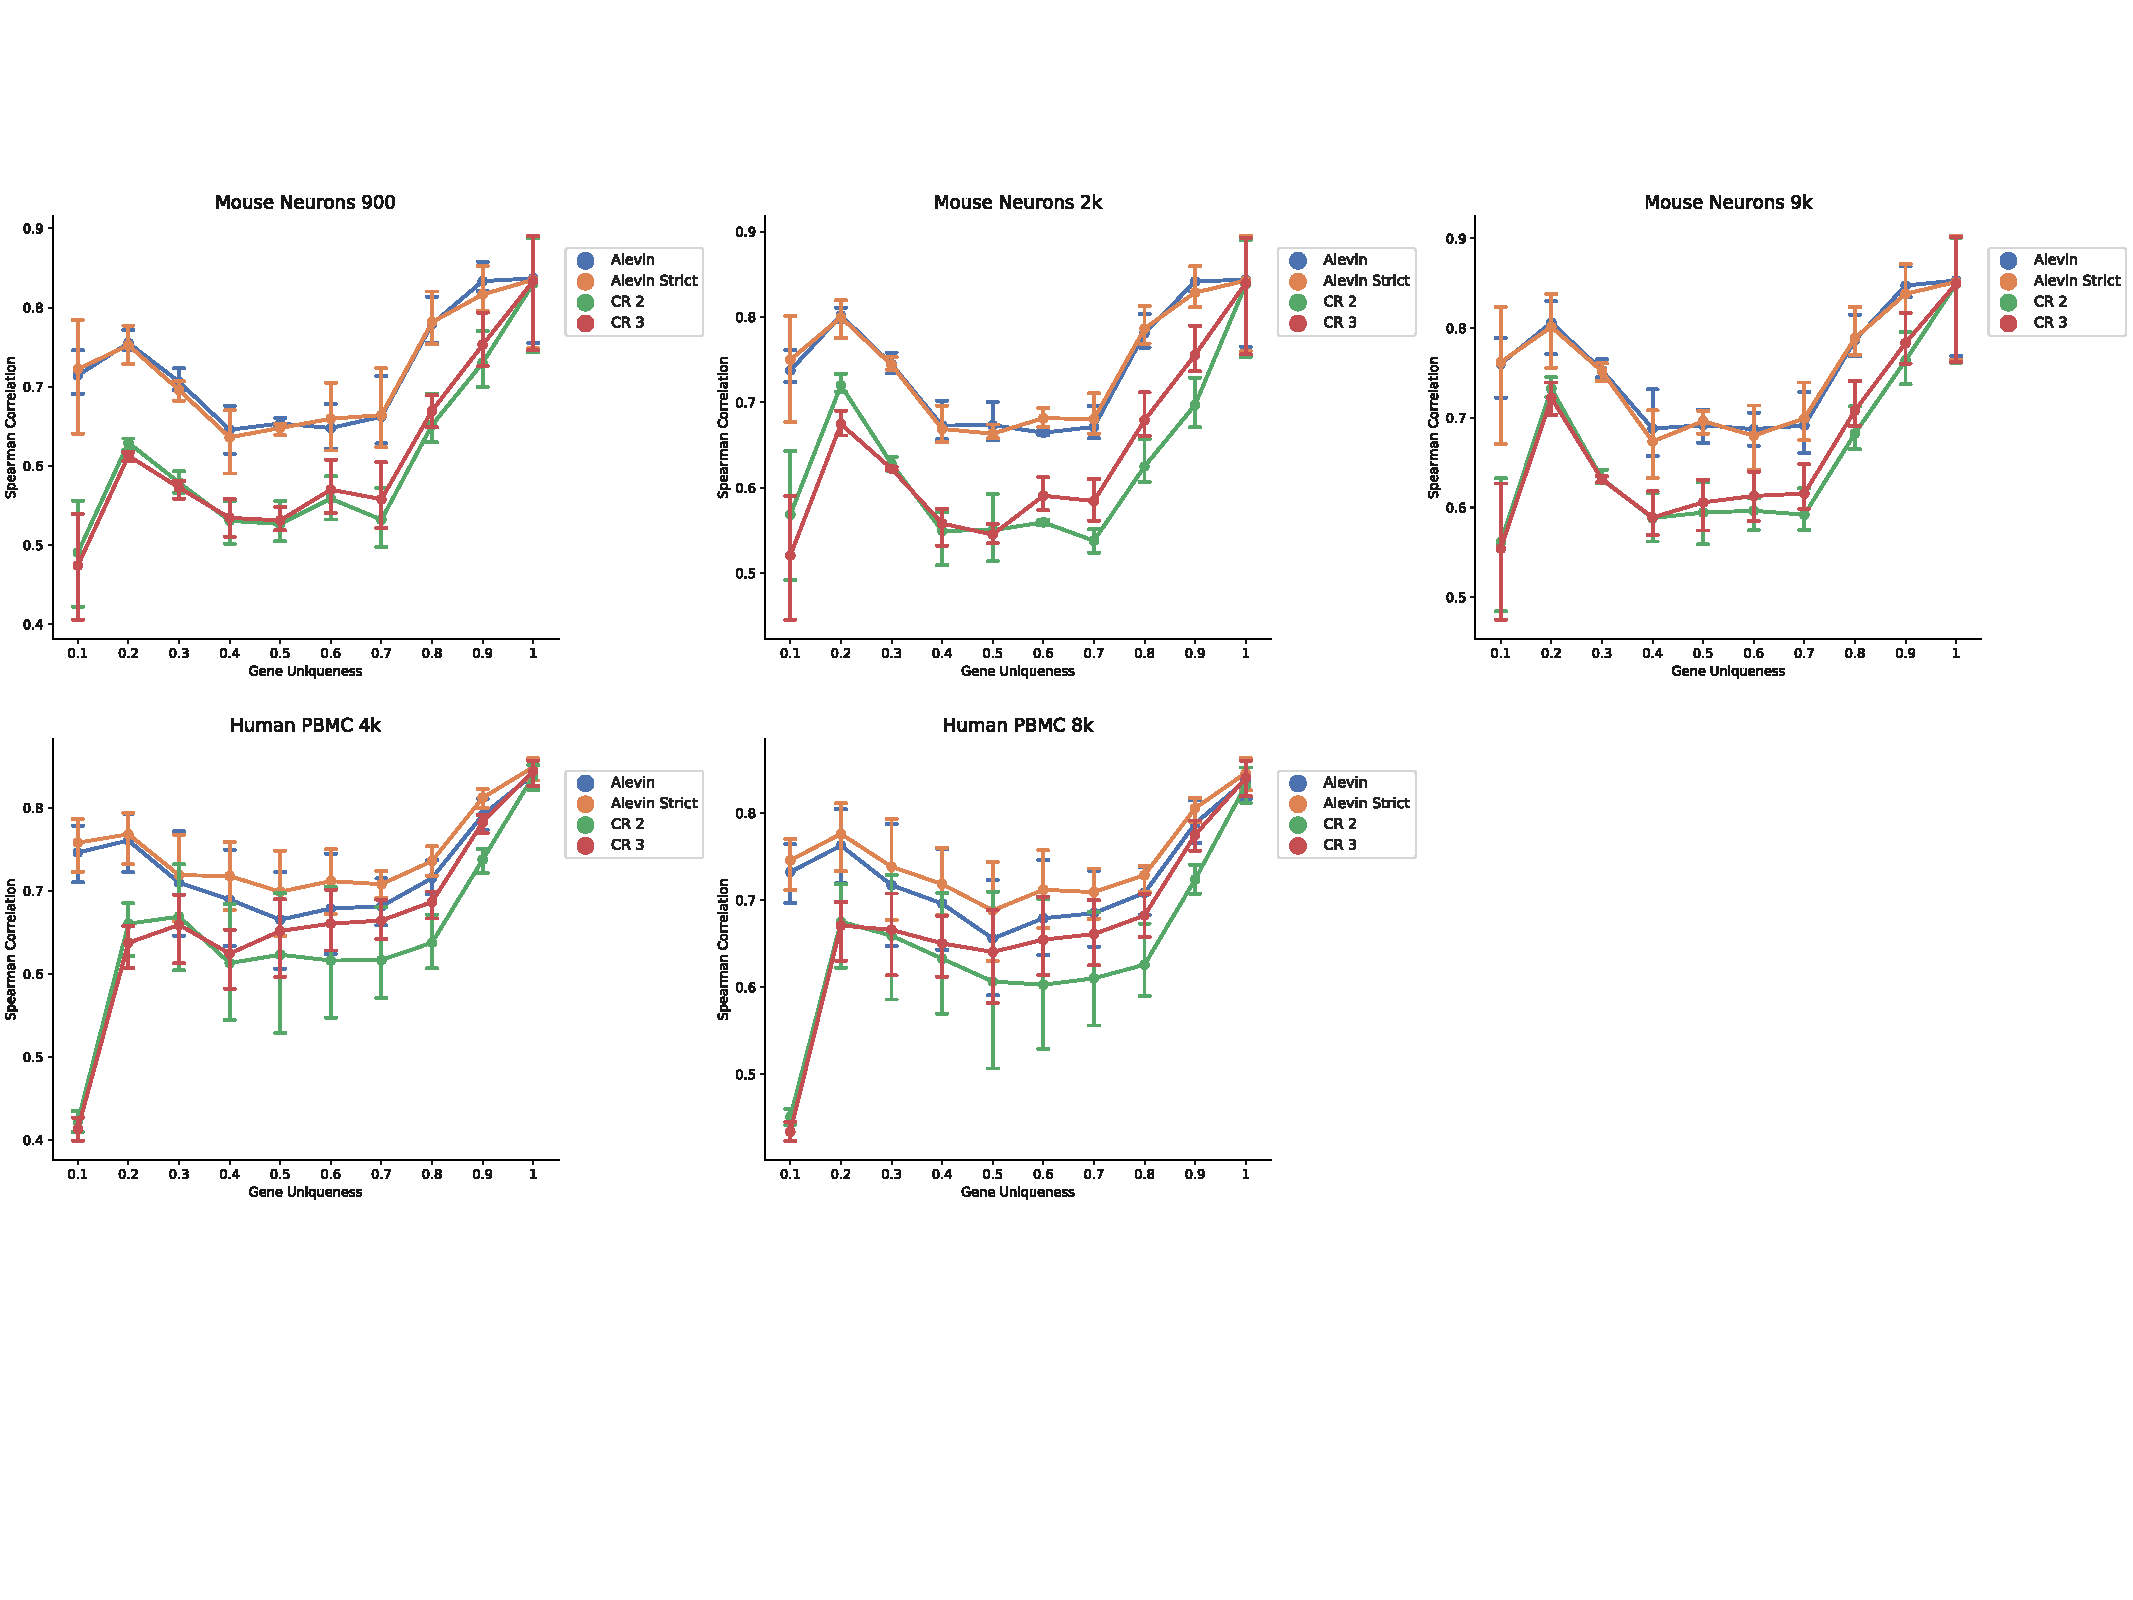
\includegraphics[width=\linewidth]{alevin/supp_combine_corr.pdf}
  \caption{The Spearman correlation between quantification estimates from different runs of \alevin and \cellr. Note that two different versions \cellr were run with the default parameters and \alevin strict refers to the same version of \alevin run with \texttt{--minScoreFraction} set to 0.95 and \texttt{--consensusSlack} set to 0.99. These parameters in \alevin make the mapping filter strict and allows fewer spurious mappings.}
  \label{suppfig1}
\end{figure*}

\begin{figure*}[!htb]
    \centering
  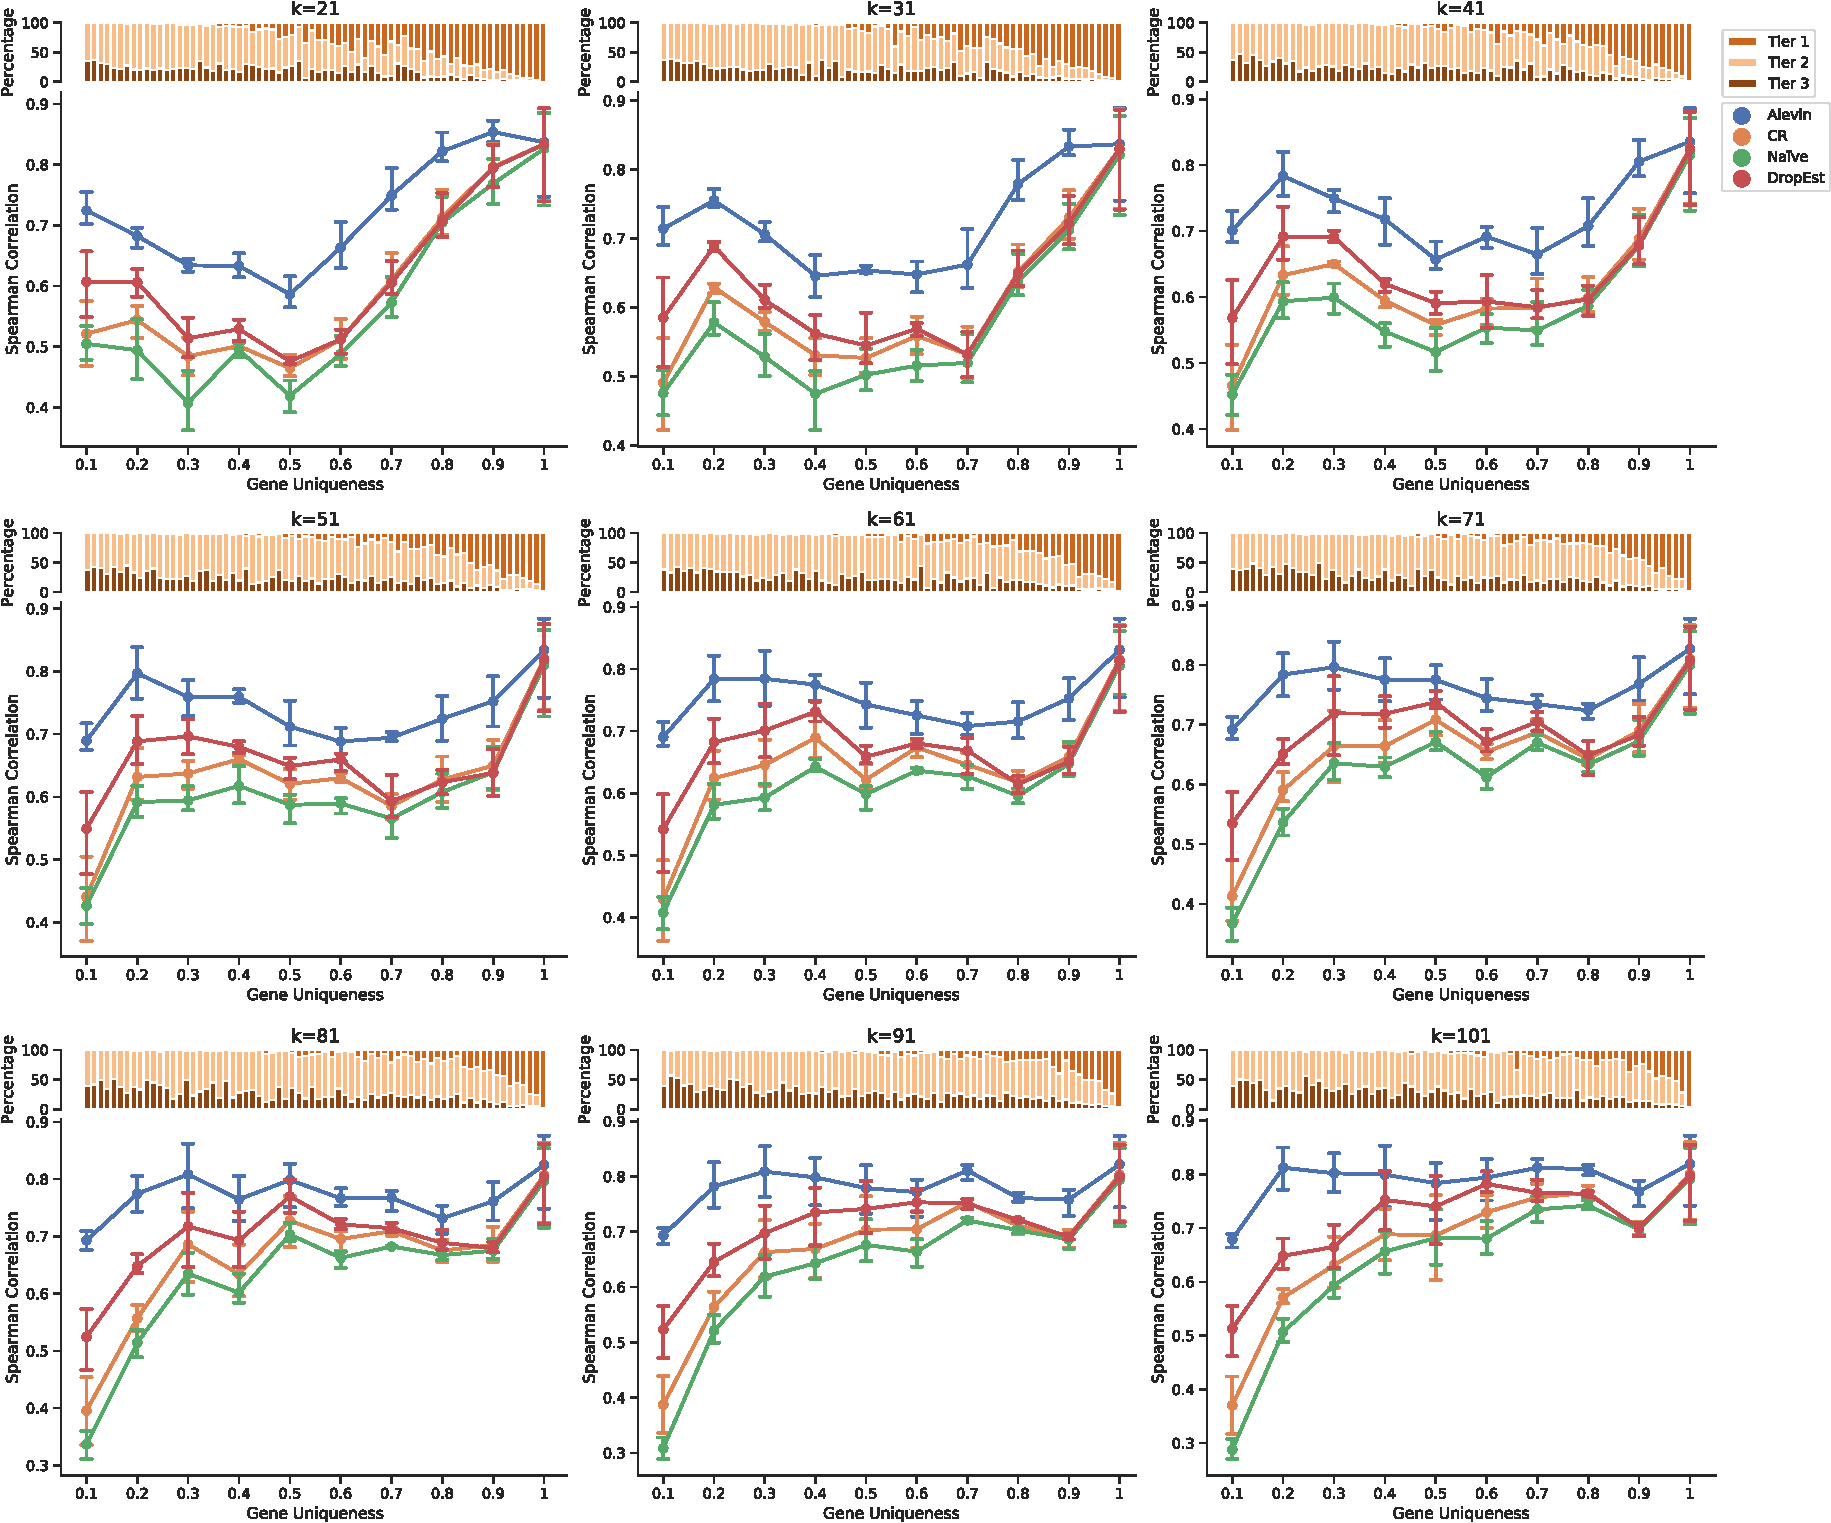
\includegraphics[width=\linewidth]{alevin/supp_combine_uniq.pdf}
  \caption{Correlation plots for the mouse neuronal 900 dataset using different values of the k-mer size (k) to calculate gene uniqueness.}
  \label{suppfig2}
\end{figure*}

\begin{figure*}[!htb]
    \centering
  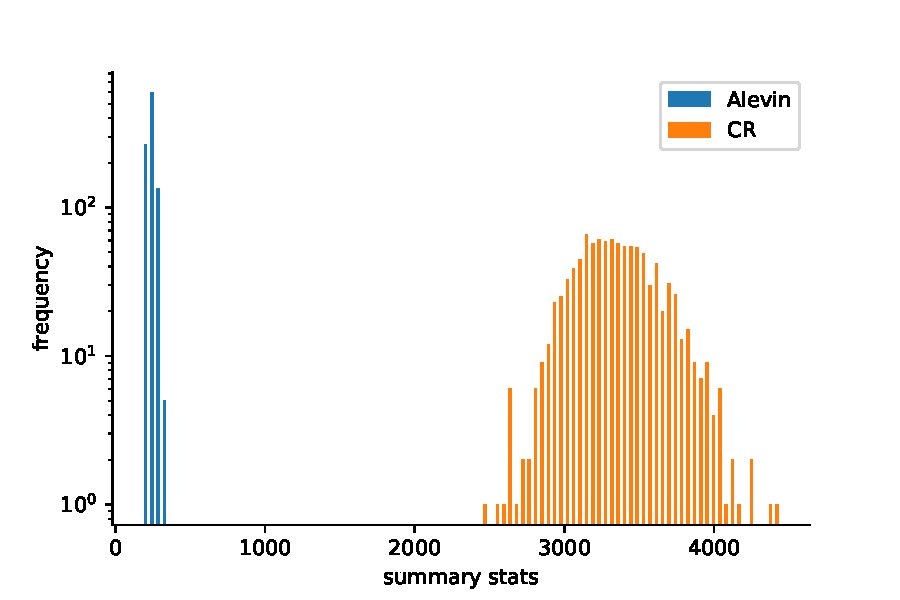
\includegraphics[width=0.8\linewidth]{alevin/supp_pvals.pdf}
  \caption{The histogram is the result of taking $1000$ samples of $100$
    cells each from the mouse neuronal 900 dataset, and looking at the sum of
    absolute differences when quantifying the data under the varying reference
    genomes (mouse vs. mouse and human combined).}
  \label{suppfig3}
\end{figure*}
%\chapter{Supplementary Material for \cref{alevin}}
\label{appendix-alevin}

\section{ Machine Configuration and Pipeline Replicability }
\label{sec:tool_params}

%10x v1 chemistry benchmarking has been scripted using Snakemake \cite{snakemake} and performed on an Intel(R) Xeon(R) CPU (E5-2699 v4 @2.20GHz with 44 cores and 56MB L3 cache) with 512GB RAM and a 4TB TOSHIBA MG03ACA4 ATA HDD running Ubuntu 16.10.

10x v2 chemistry benchmarking has been scripted using CGATCore (https://github.com/cgat-developers/cgat-core). The full pipeline and analysis are performed using Stony Brook's seawulf cluster with 164 Intel Xeon E5-2683v3 CPUs.

For all analyses, the genome and gtf versions used for human datasets was GENCODE release 27, GRCh38.p10 and for mouse datasets was GENCODE release M16, GRCm38.p5. All transcriptome files were generated using these with ``rsem-prepare-reference".

\textbf{\cellr (v2.2.0):} The following additional flags were used, as recommended by the \cellr guidelines: \texttt{--nosecondary --expect-cells NumCells}, where NumCells is 10,000 for PBMC 8k and Neurons 9k,
5,000 for PBMC 4k, 2,000 for Neurons 2k and Neurons 900.

\textbf{\Alevin (v0.13.0):} Run with default parameters with the chromium protocol and \texttt{--keepDuplicates} flags and the \texttt{-lISR} to specify strandedness. The mRNA and rRNA lists were obtained from the relevant annotation files and passed as input. Experiments on v1 chemistry can be run using the same flags but with the \texttt{--gemcode} protocol flag.  \Alevin also supports 10x v3 chemistry via the command-line flag \texttt{--chromiumV3}.

\textbf{STAR (v2.6.0a):} The following flag was used, as recommended by the guidelines of UMI-tools: \\ \texttt{--outFilterMultimapNmax 1} 

\textbf{featureCounts (v1.6.3):} This was run to obtain an output BAM file and with stranded input (\texttt{-s 1}).

\textbf{UMI-tools (v0.5.4):} The extract command was used to get the CBs/UMIs, when provided with an external CB whitelist, and attach it to the corresponding reads. The following flags were used in the count command to obtain the per cell gene count matrix: \texttt{--gene-tag=XT --wide-format-cell-counts}

\dropest (v0.8.5): This was run with the default parameters on the 10x BAM files and the predicted cell counts from \cellr were used as input.

\textbf{Dropseq utils (v2.0.0):} All the commands were run as recommended by the authors in the tool's manual.

The bulk datasets were quantified using Bowtie2 and RSEM, run as follows:

\textbf{Bowtie2 (v2.3.4.3):} The following flags were used, as recommended in the guidelines of RSEM: \texttt{--sensitive --dpad 0 --gbar 99999999 --mp 1,1 --np 1 --score-min L,0,-0.1 --no-mixed \\ --no-discordant}

\textbf{RSEM (v1.3.1):} Run with default parameters.


%%%%%%%%%%%%%%%%%%%%%%%%%%%%%%%%%%%%%%%%%%%%%%
%%                                          %%
%% Backmatter begins here                   %%
%%                                          %%
%%%%%%%%%%%%%%%%%%%%%%%%%%%%%%%%%%%%%%%%%%%%%%

\section{Availability of data and materials}
\Alevin is implemented in \texttt{C++14} and is released under the GNU General Public License v3.0. The source code as used in the chapter has been deposited in archived format at \url{https://doi.org/10.5281/zenodo.2583275}~\citep{scode} and the latest code is available at \url{https://github.com/COMBINE-lab/salmon}~\citep{alvgit}. The output quantification results of all the tools used in the validation of \alevin-pipeline have been deposited in archived format at \url{https://doi.org/10.5281/zenodo.2583228}~\citep{vdata}.

All the single cell 10x datasets used in the chapter are taken from \url{https://support.10xgenomics.com/single-cell-gene-expression/datasets}~\citep{v2data} and the DropSeq data is from SRR1853180. The relevant accessions for the bulk RNA-seq datasets used for the validation are listed in~\Cref{suptab:bulkmmRate}.

\newpage
\section{Additional Figures}
\begin{figure*}[!htb]
    \centering
  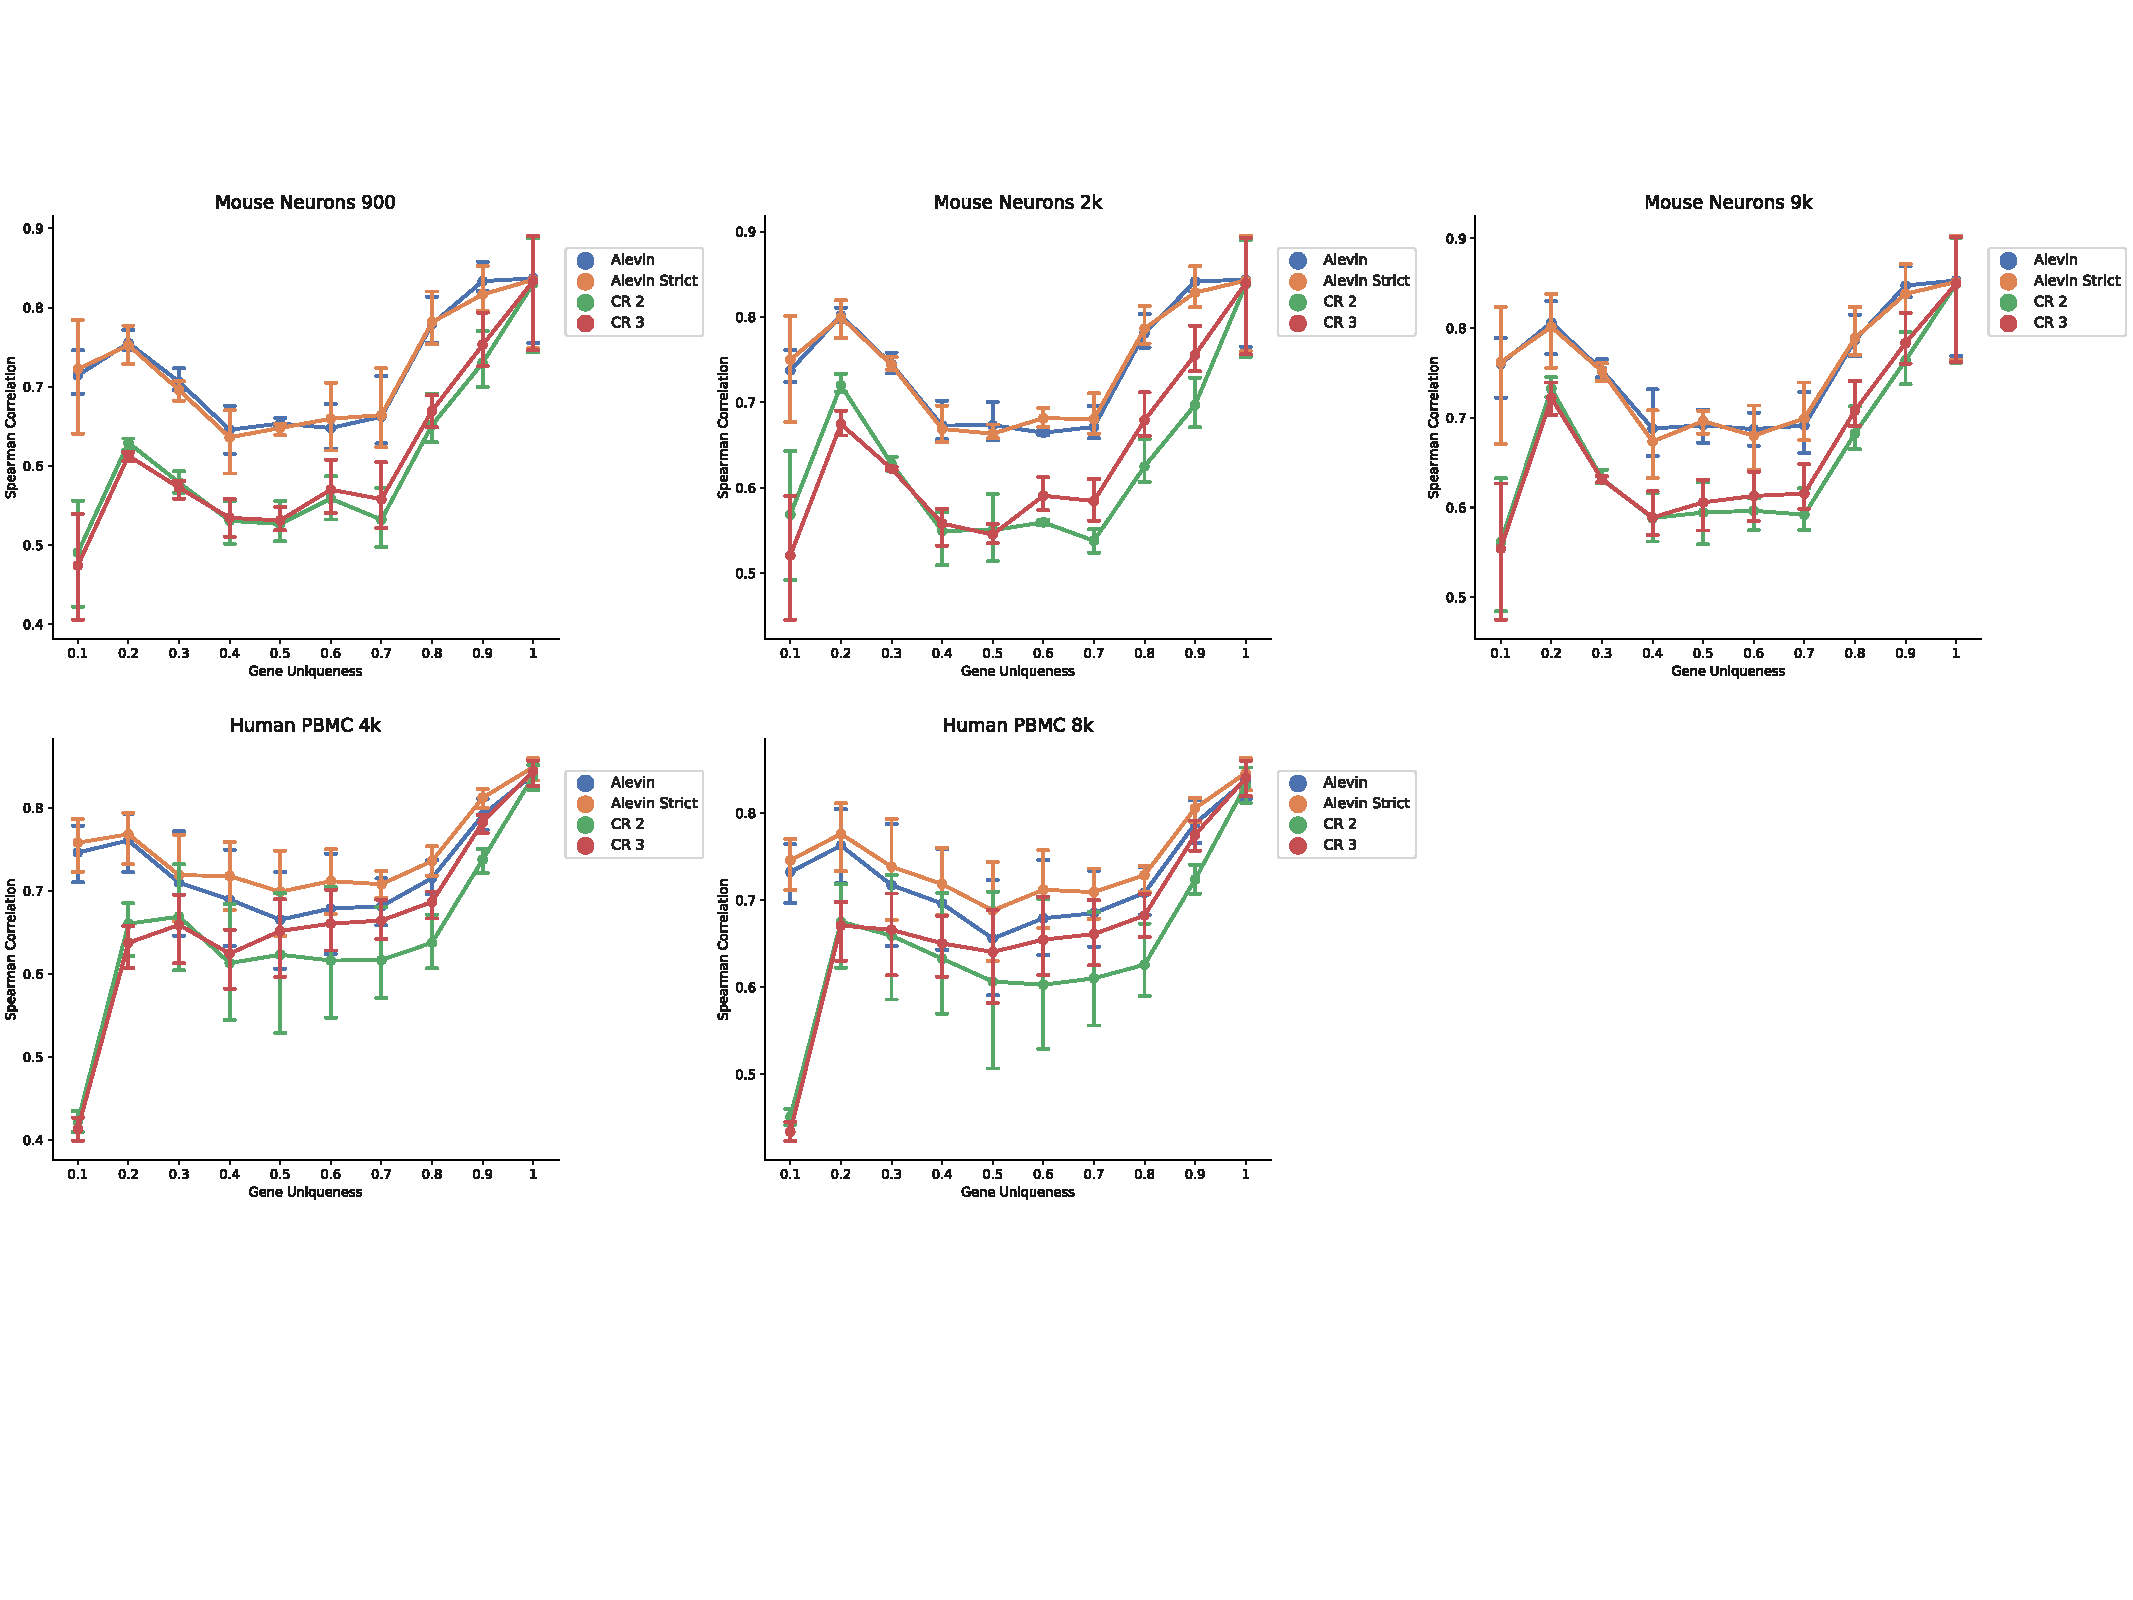
\includegraphics[width=\linewidth]{alevin/supp_combine_corr.pdf}
  \caption{The Spearman correlation between quantification estimates from different runs of \alevin and \cellr. Note that two different versions \cellr were run with the default parameters and \alevin strict refers to the same version of \alevin run with \texttt{--minScoreFraction} set to 0.95 and \texttt{--consensusSlack} set to 0.99. These parameters in \alevin make the mapping filter strict and allows fewer spurious mappings.}
  \label{suppfig1}
\end{figure*}

\begin{figure*}[!htb]
    \centering
  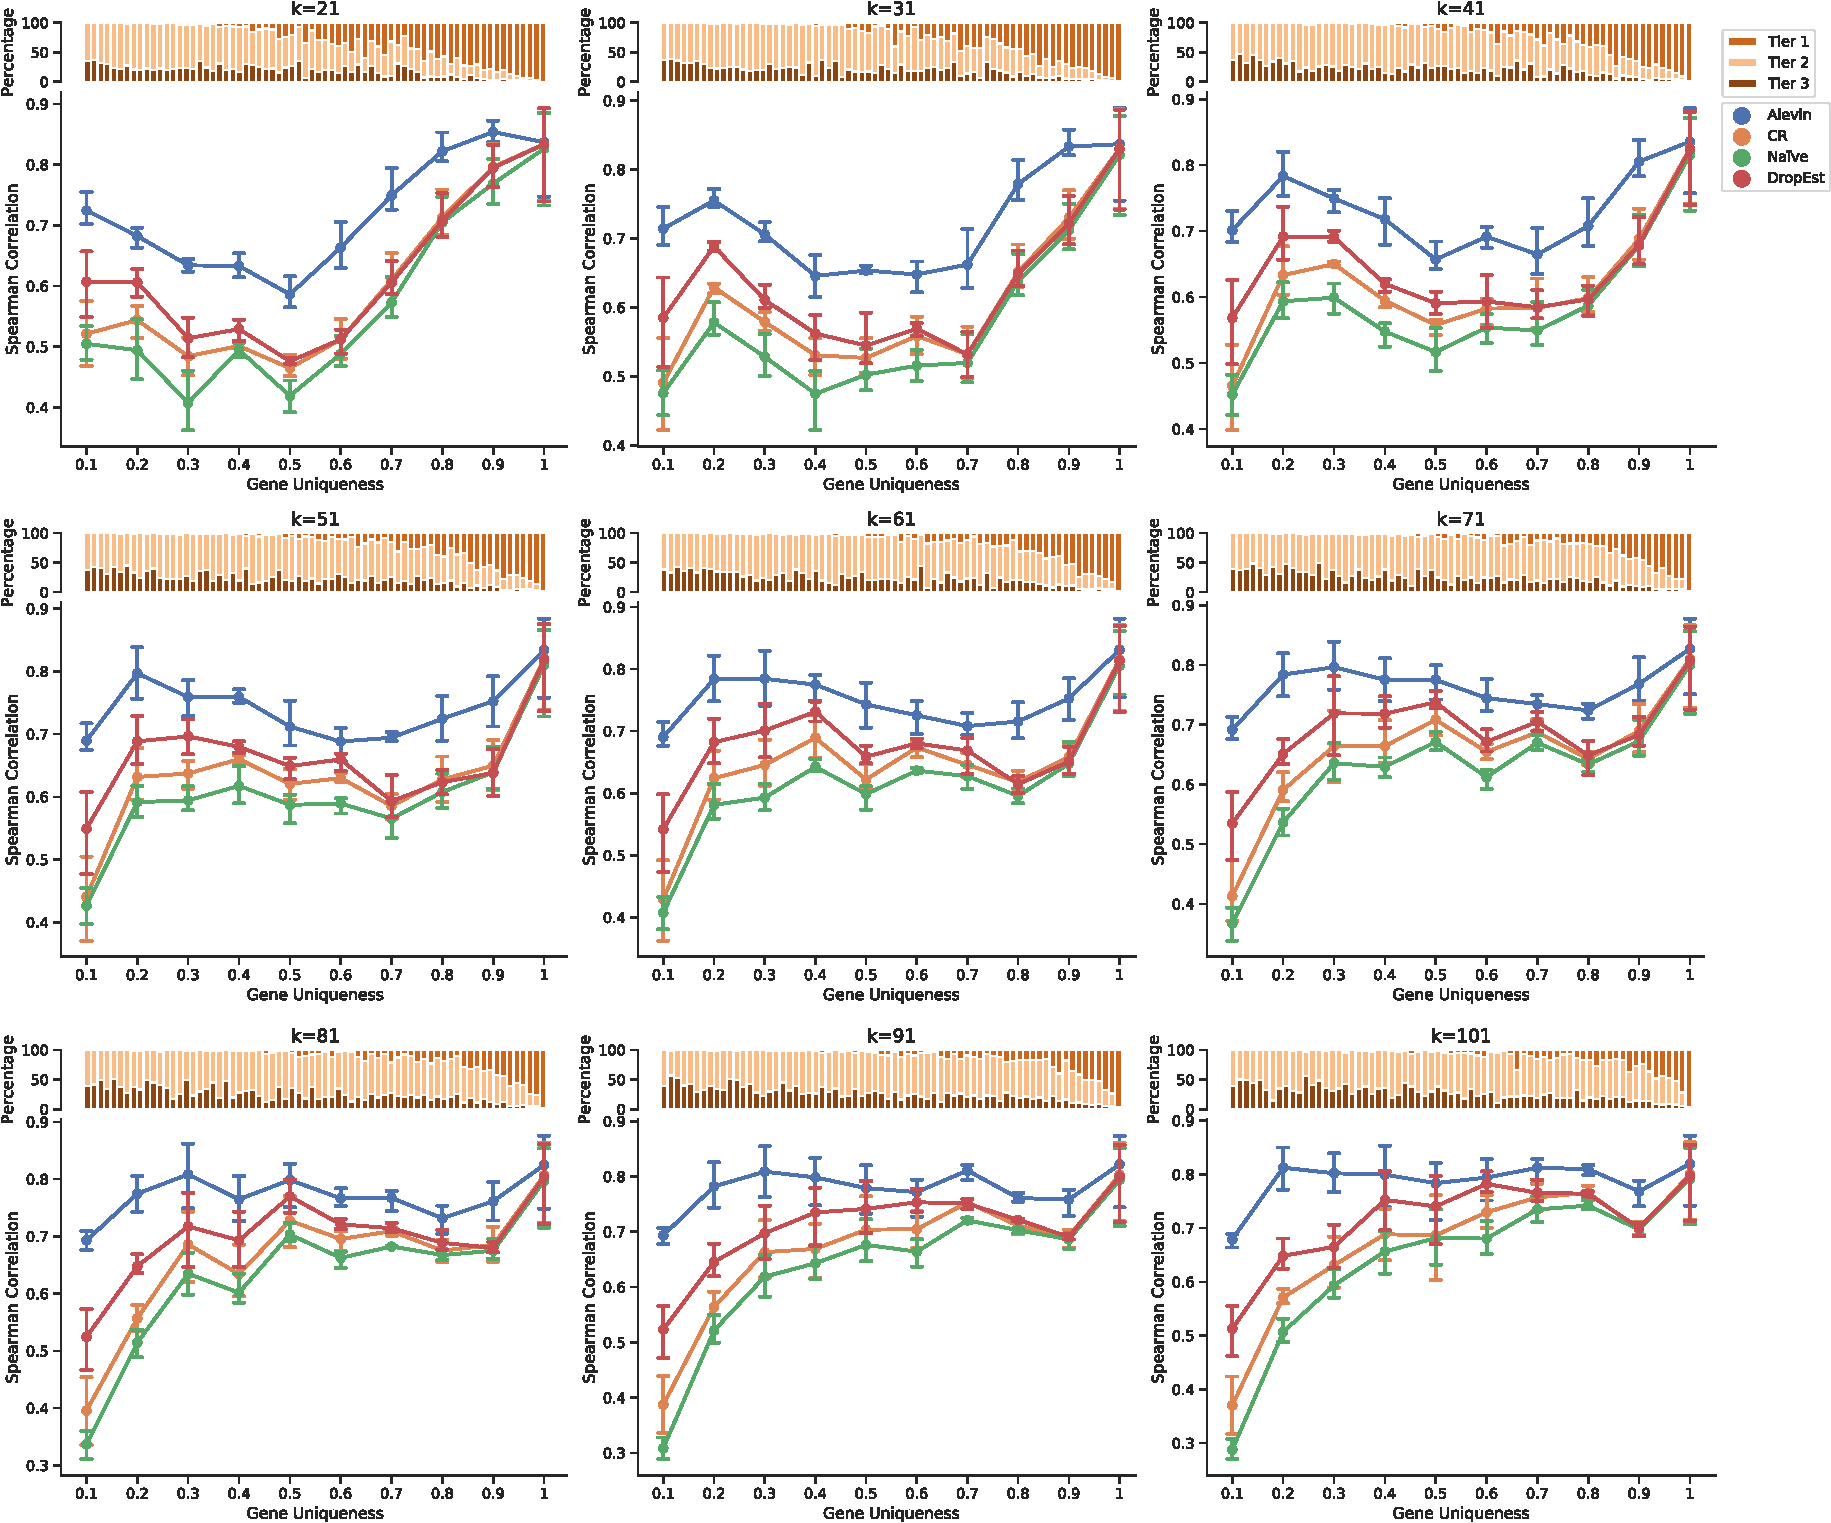
\includegraphics[width=\linewidth]{alevin/supp_combine_uniq.pdf}
  \caption{Correlation plots for the mouse neuronal 900 dataset using different values of the k-mer size (k) to calculate gene uniqueness.}
  \label{suppfig2}
\end{figure*}

\begin{figure*}[!htb]
    \centering
  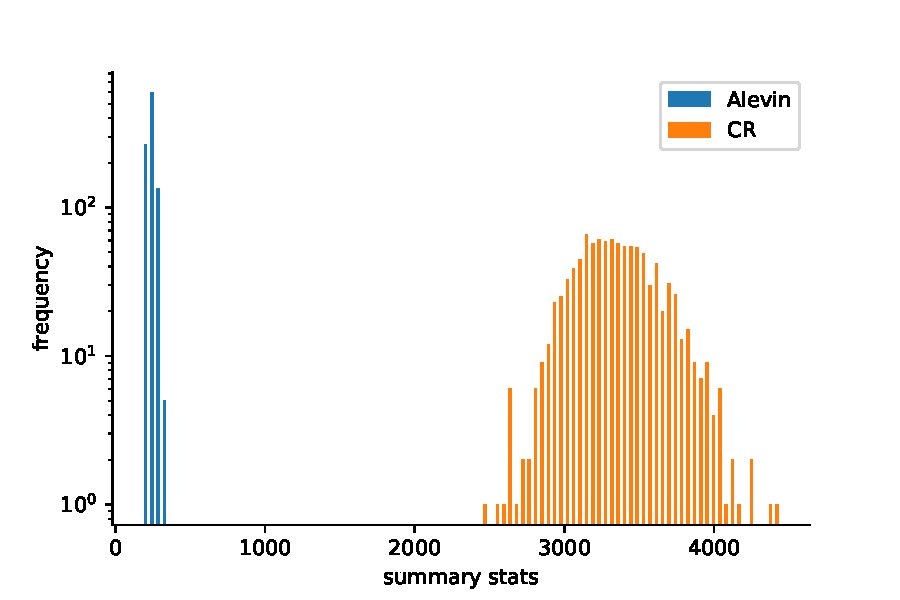
\includegraphics[width=0.8\linewidth]{alevin/supp_pvals.pdf}
  \caption{The histogram is the result of taking $1000$ samples of $100$
    cells each from the mouse neuronal 900 dataset, and looking at the sum of
    absolute differences when quantifying the data under the varying reference
    genomes (mouse vs. mouse and human combined).}
  \label{suppfig3}
\end{figure*}

%----------------------------------------------------------------------------------------
%    BIBLIOGRAPHY
%----------------------------------------------------------------------------------------

\printbibliography[heading=bibintoc]

%----------------------------------------------------------------------------------------

\end{document}  
